\chapter{Stellar Component}
	\label{cha:stellar}


The rest of this chapter is structured as follows: firstly we present the kinematic maps for the stellar component of the galaxy (section \ref{sec:stellarKin}) with a brief description of each galaxy and a look at how they fit on the $\lambda_R$--ellipticity plane, then, in section \ref{sec:pop} we investigate the stellar populations using the absorption line strength. We conclude by looking at the odd-one-out of the sample NGC 612 in section \ref{sec:NGC612}

\section{Kinematics}
	\label{sec:stellarKin}

	\subsection{Maps}
		\label{subsec:maps}

		\begin{figure*}
      \centering
      \includegraphics[width=0.245\textwidth]{Vmaps/ngc0612_stellar_sigma.png}
      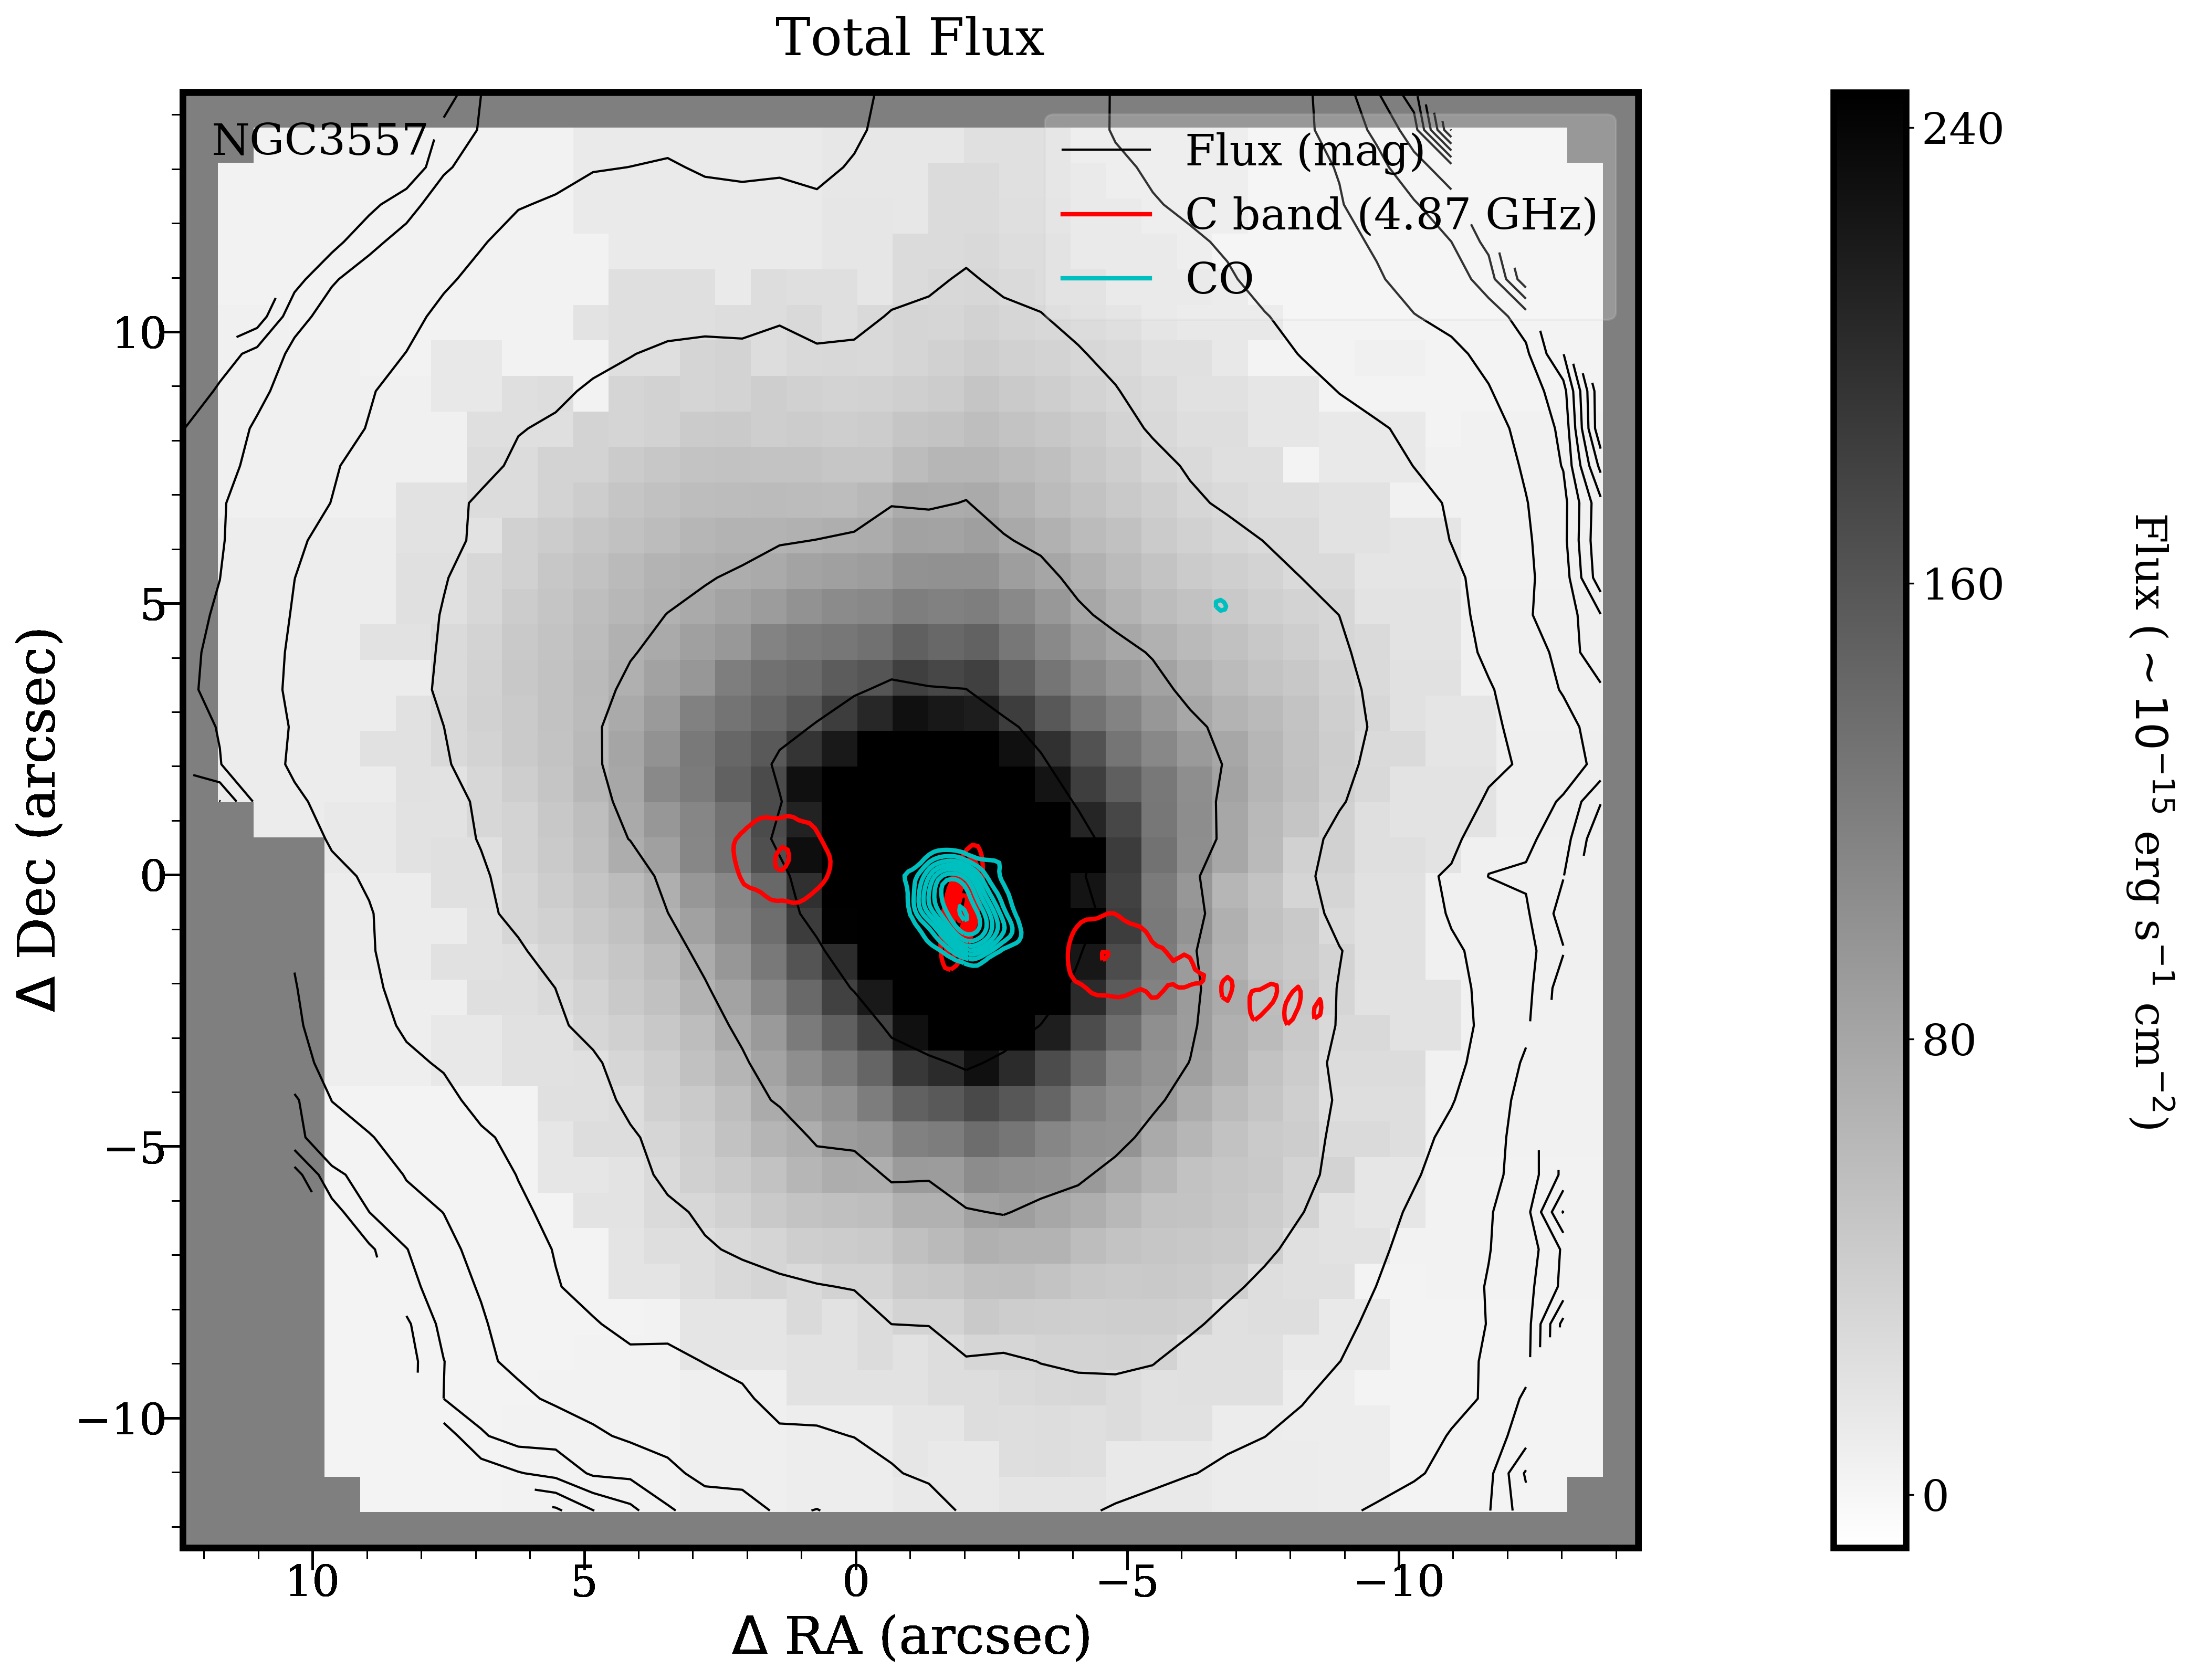
\includegraphics[width=0.245\textwidth]{Vmaps/ngc3557_stellar_img.png}
      \includegraphics[width=0.245\textwidth]{Vmaps/ngc3100_stellar_img.png}
      \includegraphics[width=0.245\textwidth]{Vmaps/ic1459_stellar_img.png}
      \includegraphics[width=0.245\textwidth]{Vmaps/pks0718-34_stellar_img.png}
      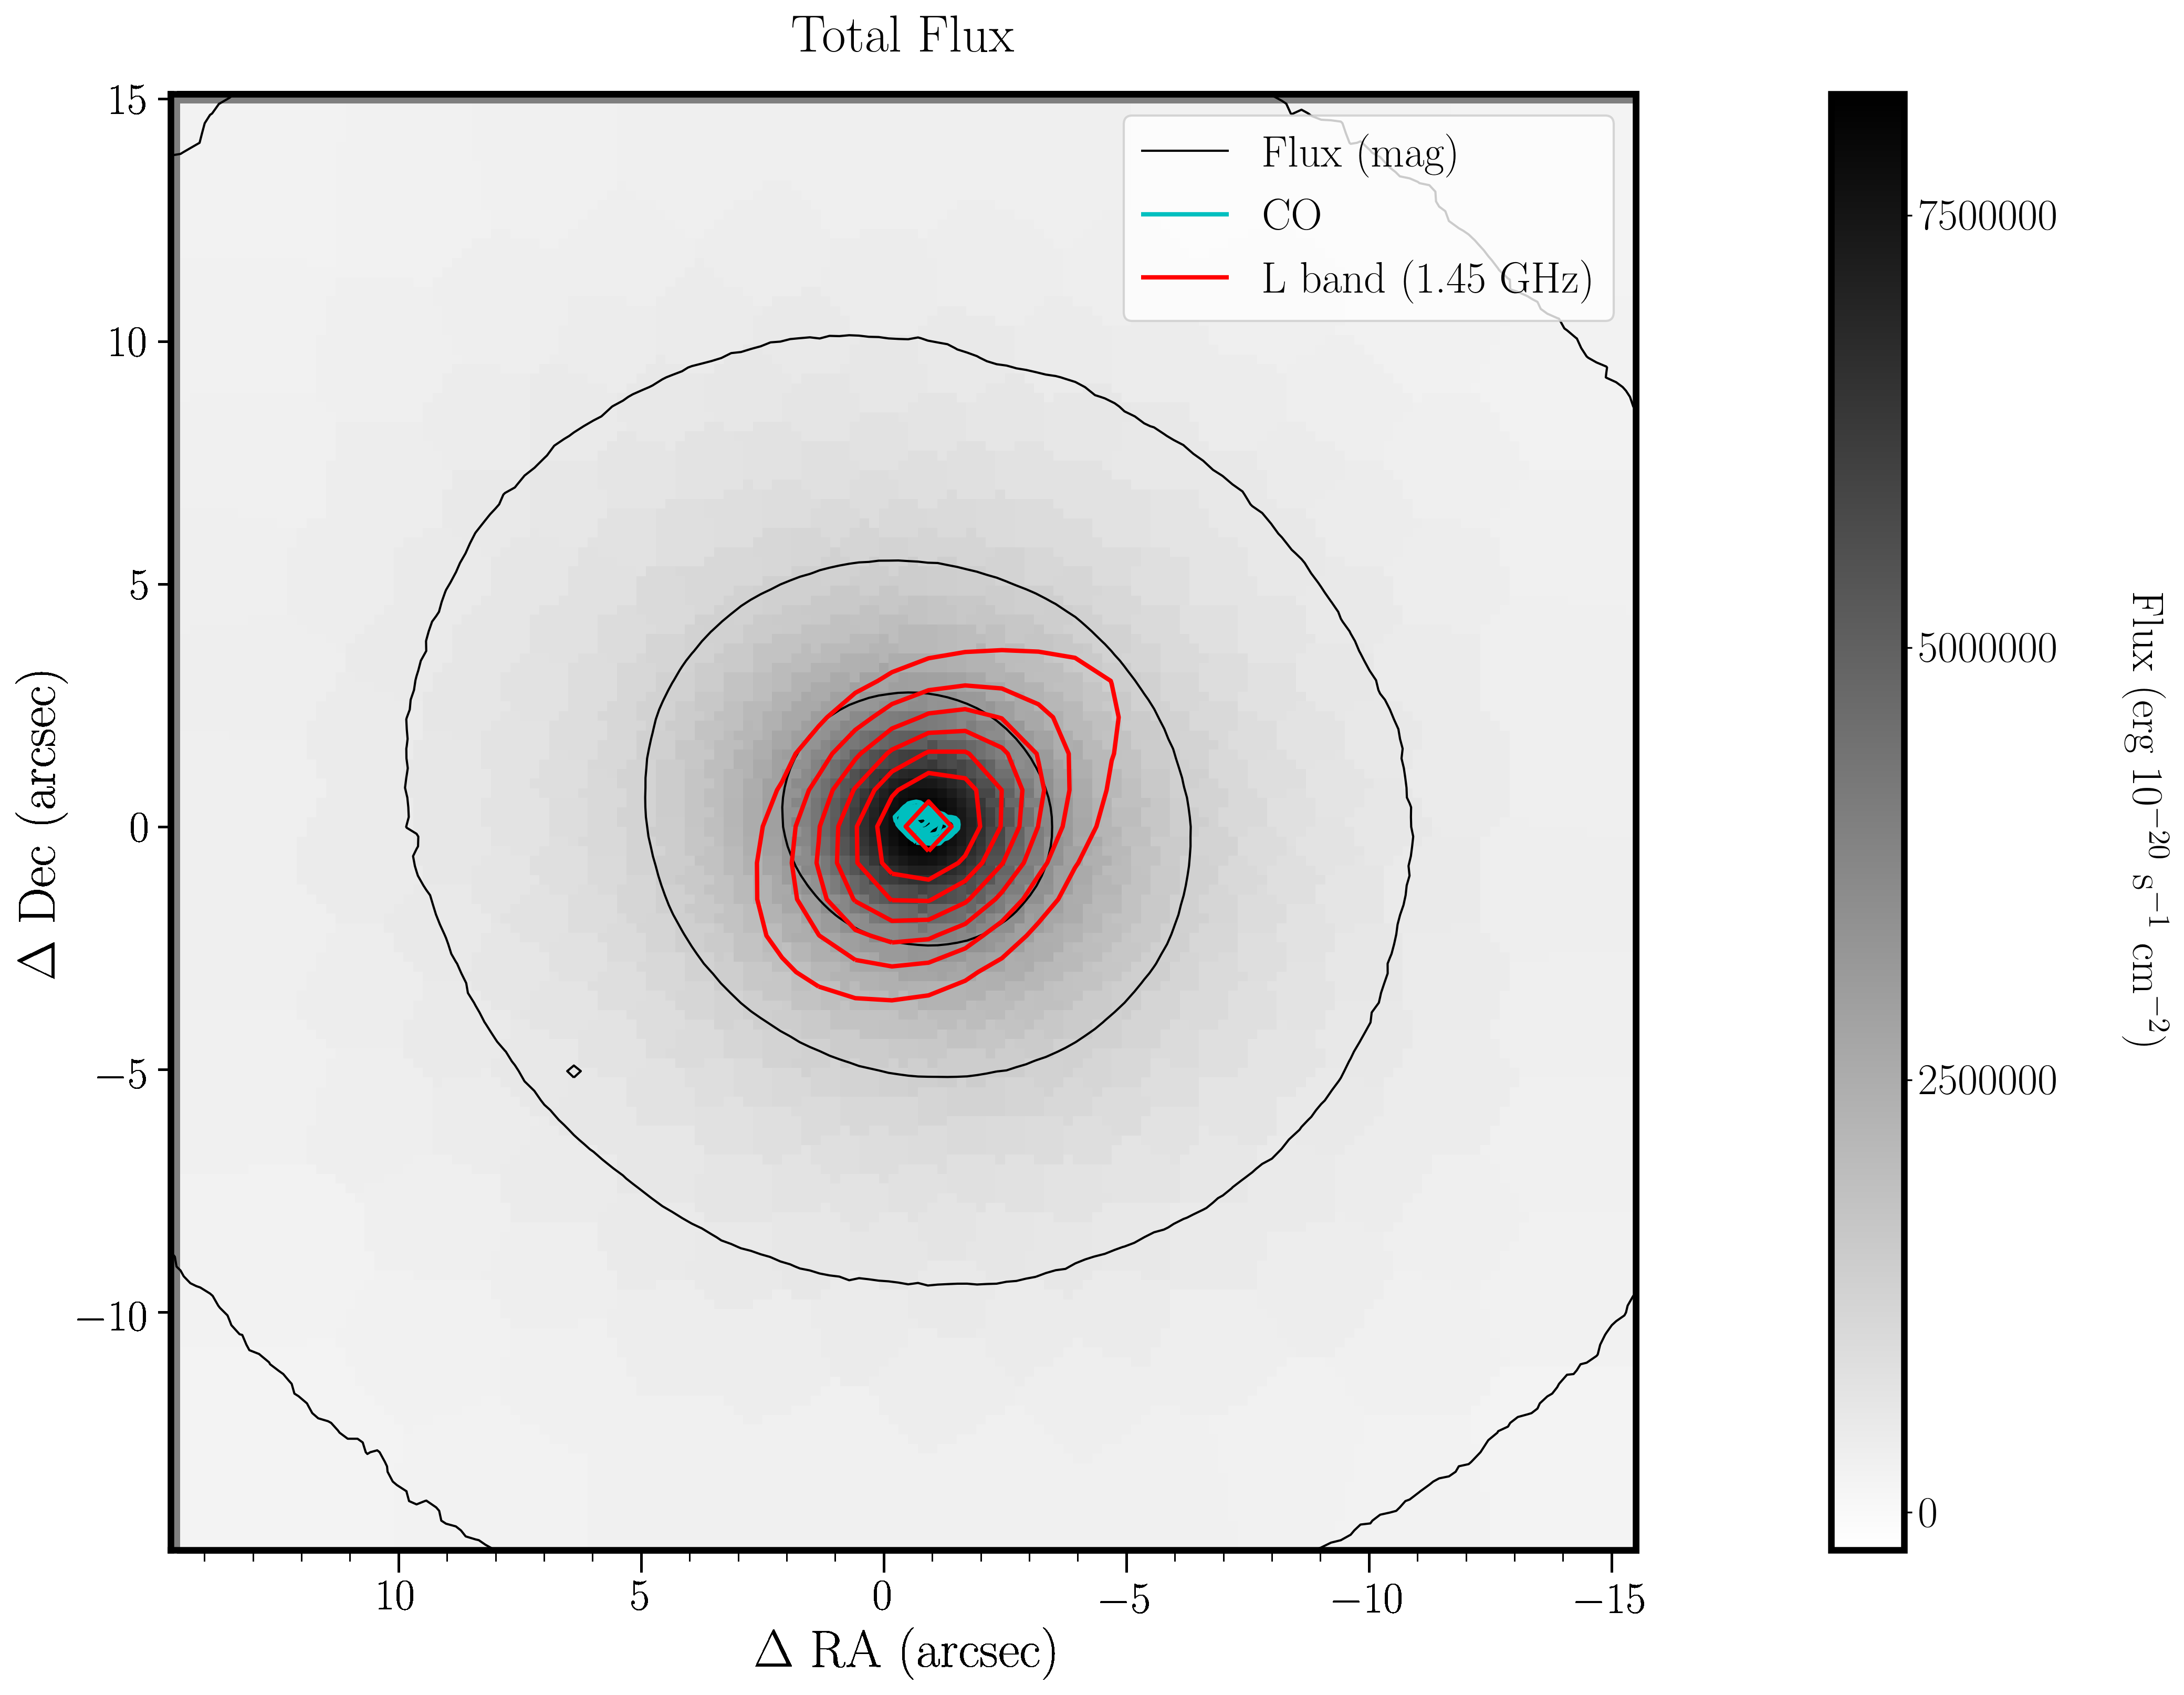
\includegraphics[width=0.245\textwidth]{Vmaps/ic4296_stellar_img.png}
      \includegraphics[width=0.245\textwidth]{Vmaps/ngc7075_stellar_img.png}
      \includegraphics[width=0.245\textwidth]{Vmaps/ic1531_stellar_img.png}
      \includegraphics[width=0.245\textwidth]{Vmaps/ngc1399_stellar_img.png}
      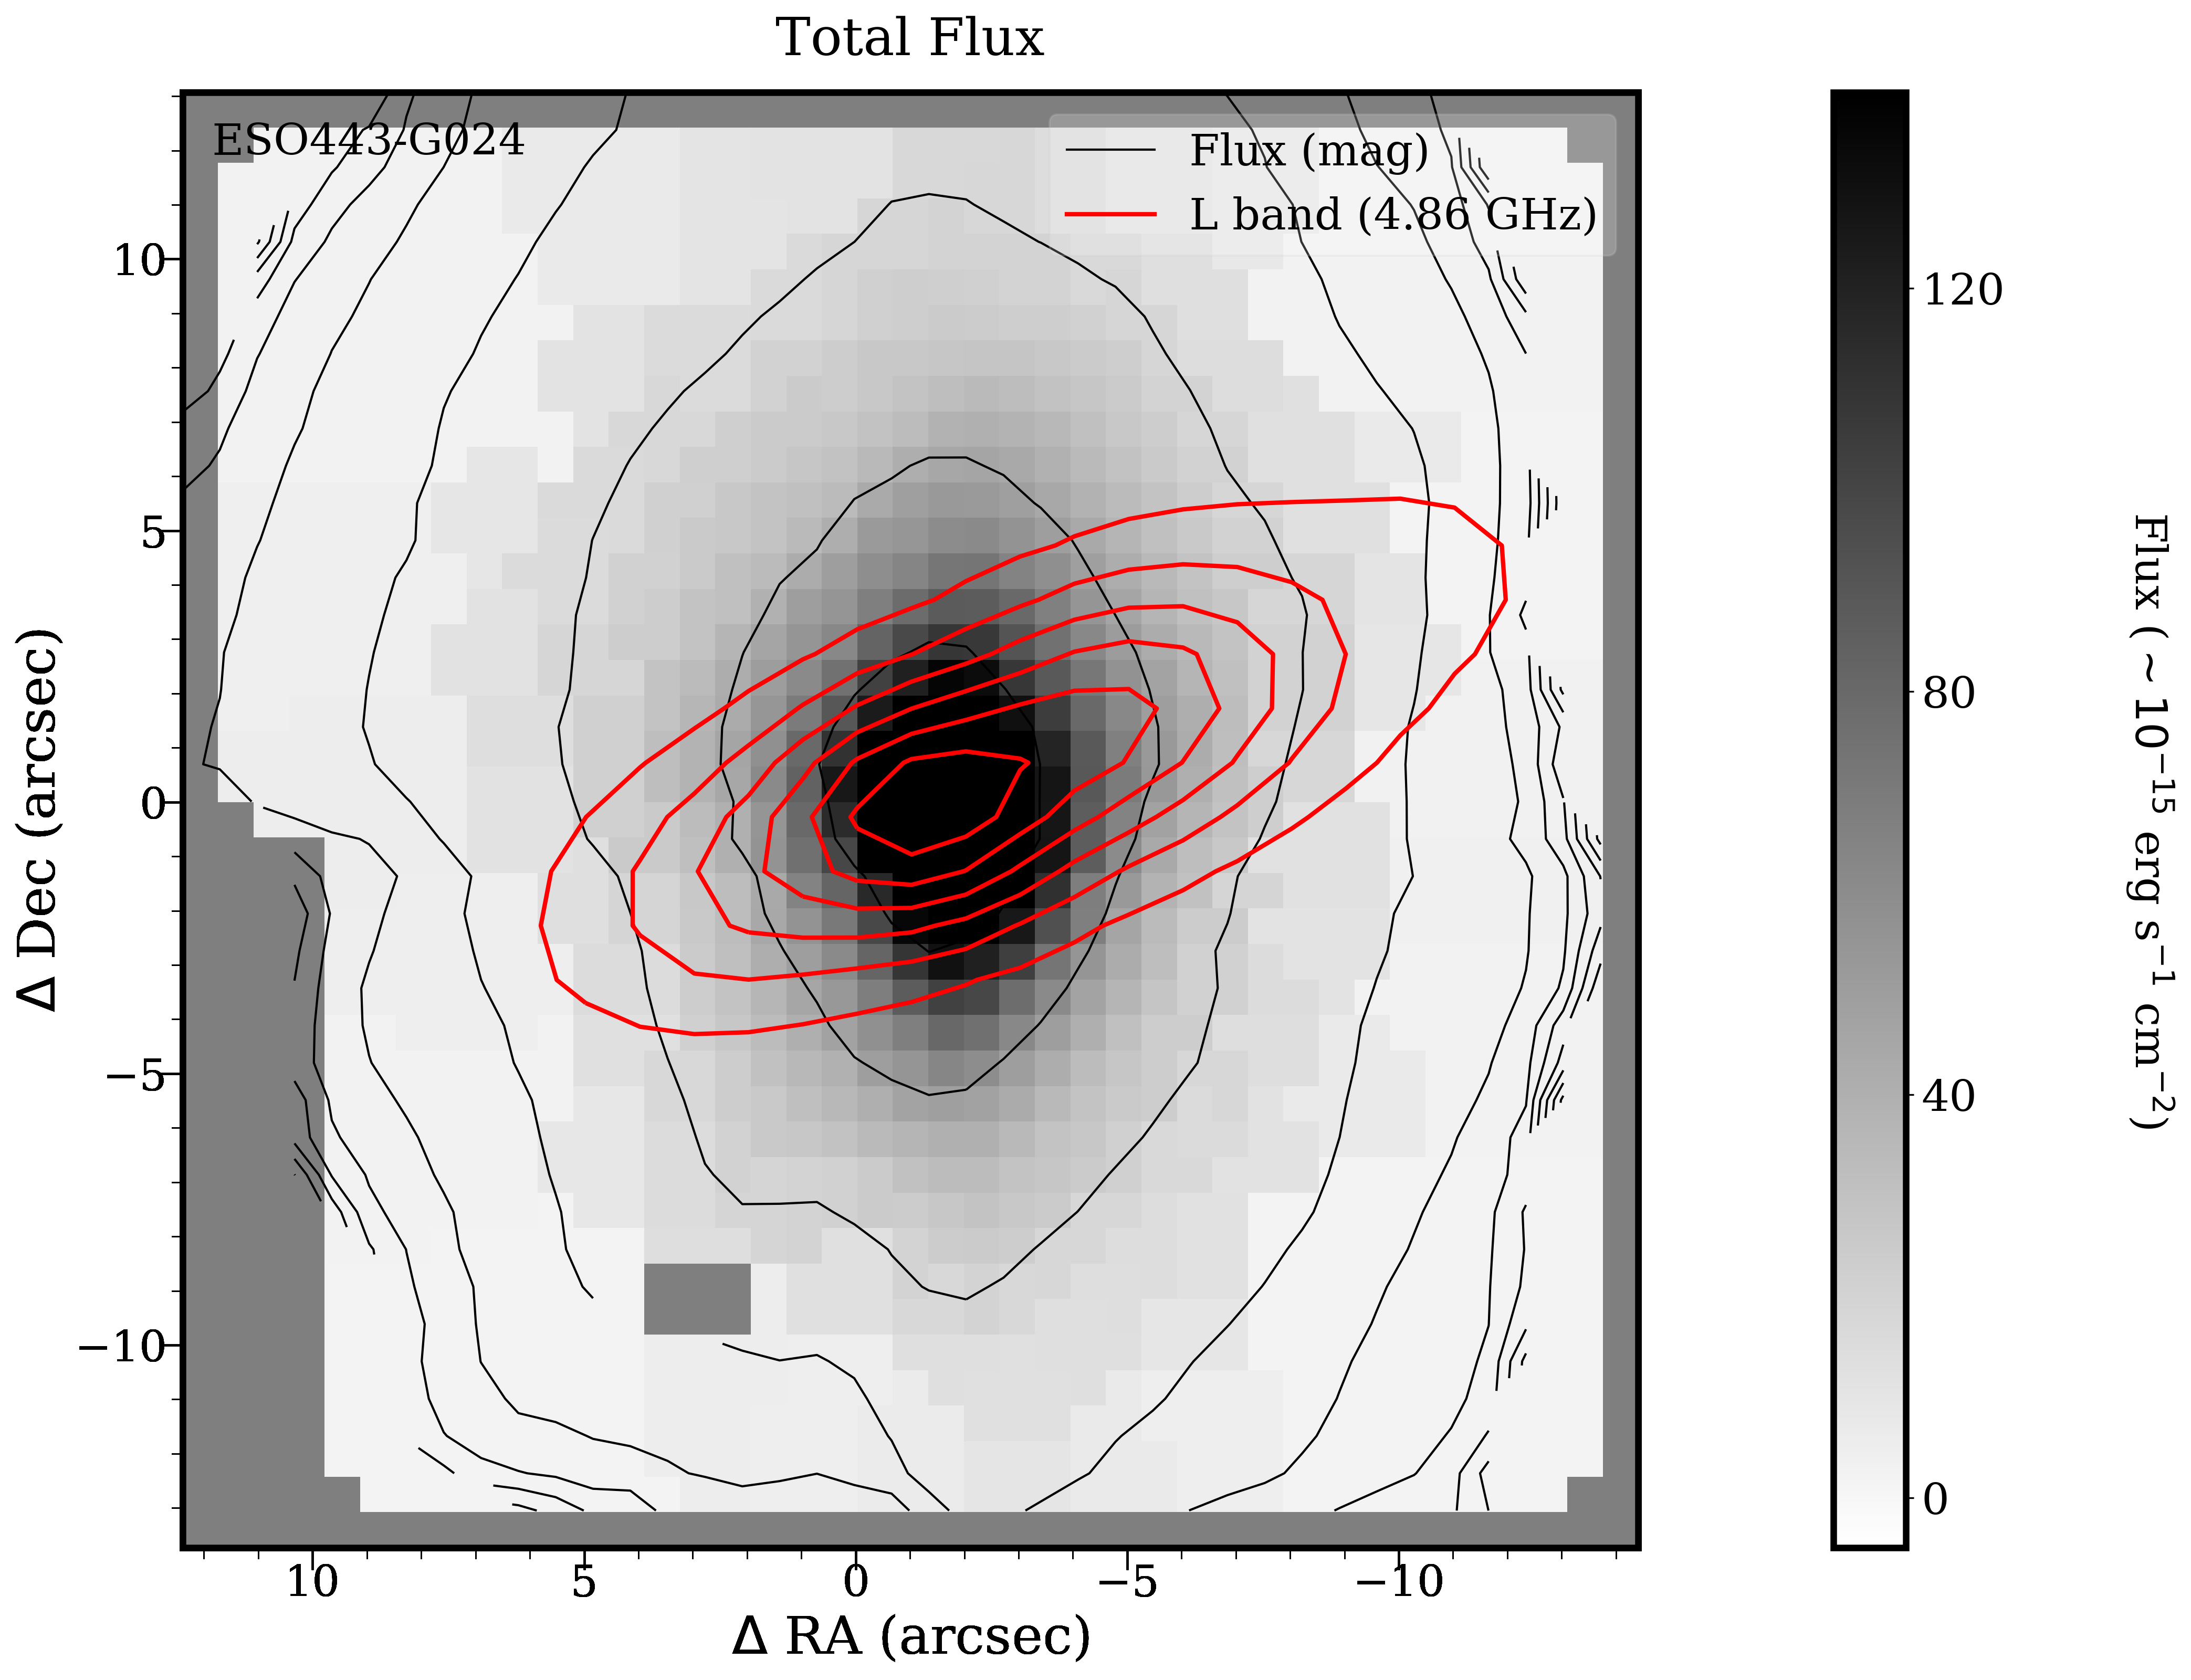
\includegraphics[width=0.245\textwidth]{Vmaps/eso443-g024_stellar_img.png}
      \caption[VIMOS images]{Image for each galaxy in the VIMOS sample. Plots are ordered roughly in peak stellar velocity, with flux contours in black, CO from ALMA in cyan and radio from VLA in red. The radio band displaied is shown in the legend of each plot and depends on what data is avaliable in the archive and which images had a similar resolution and and scale}
      \label{fig:Vstellar_img}
\end{figure*}

\begin{figure*}
      \centering
      \includegraphics[width=0.245\textwidth]{Vmaps/ngc0612_stellar_vel.png}
      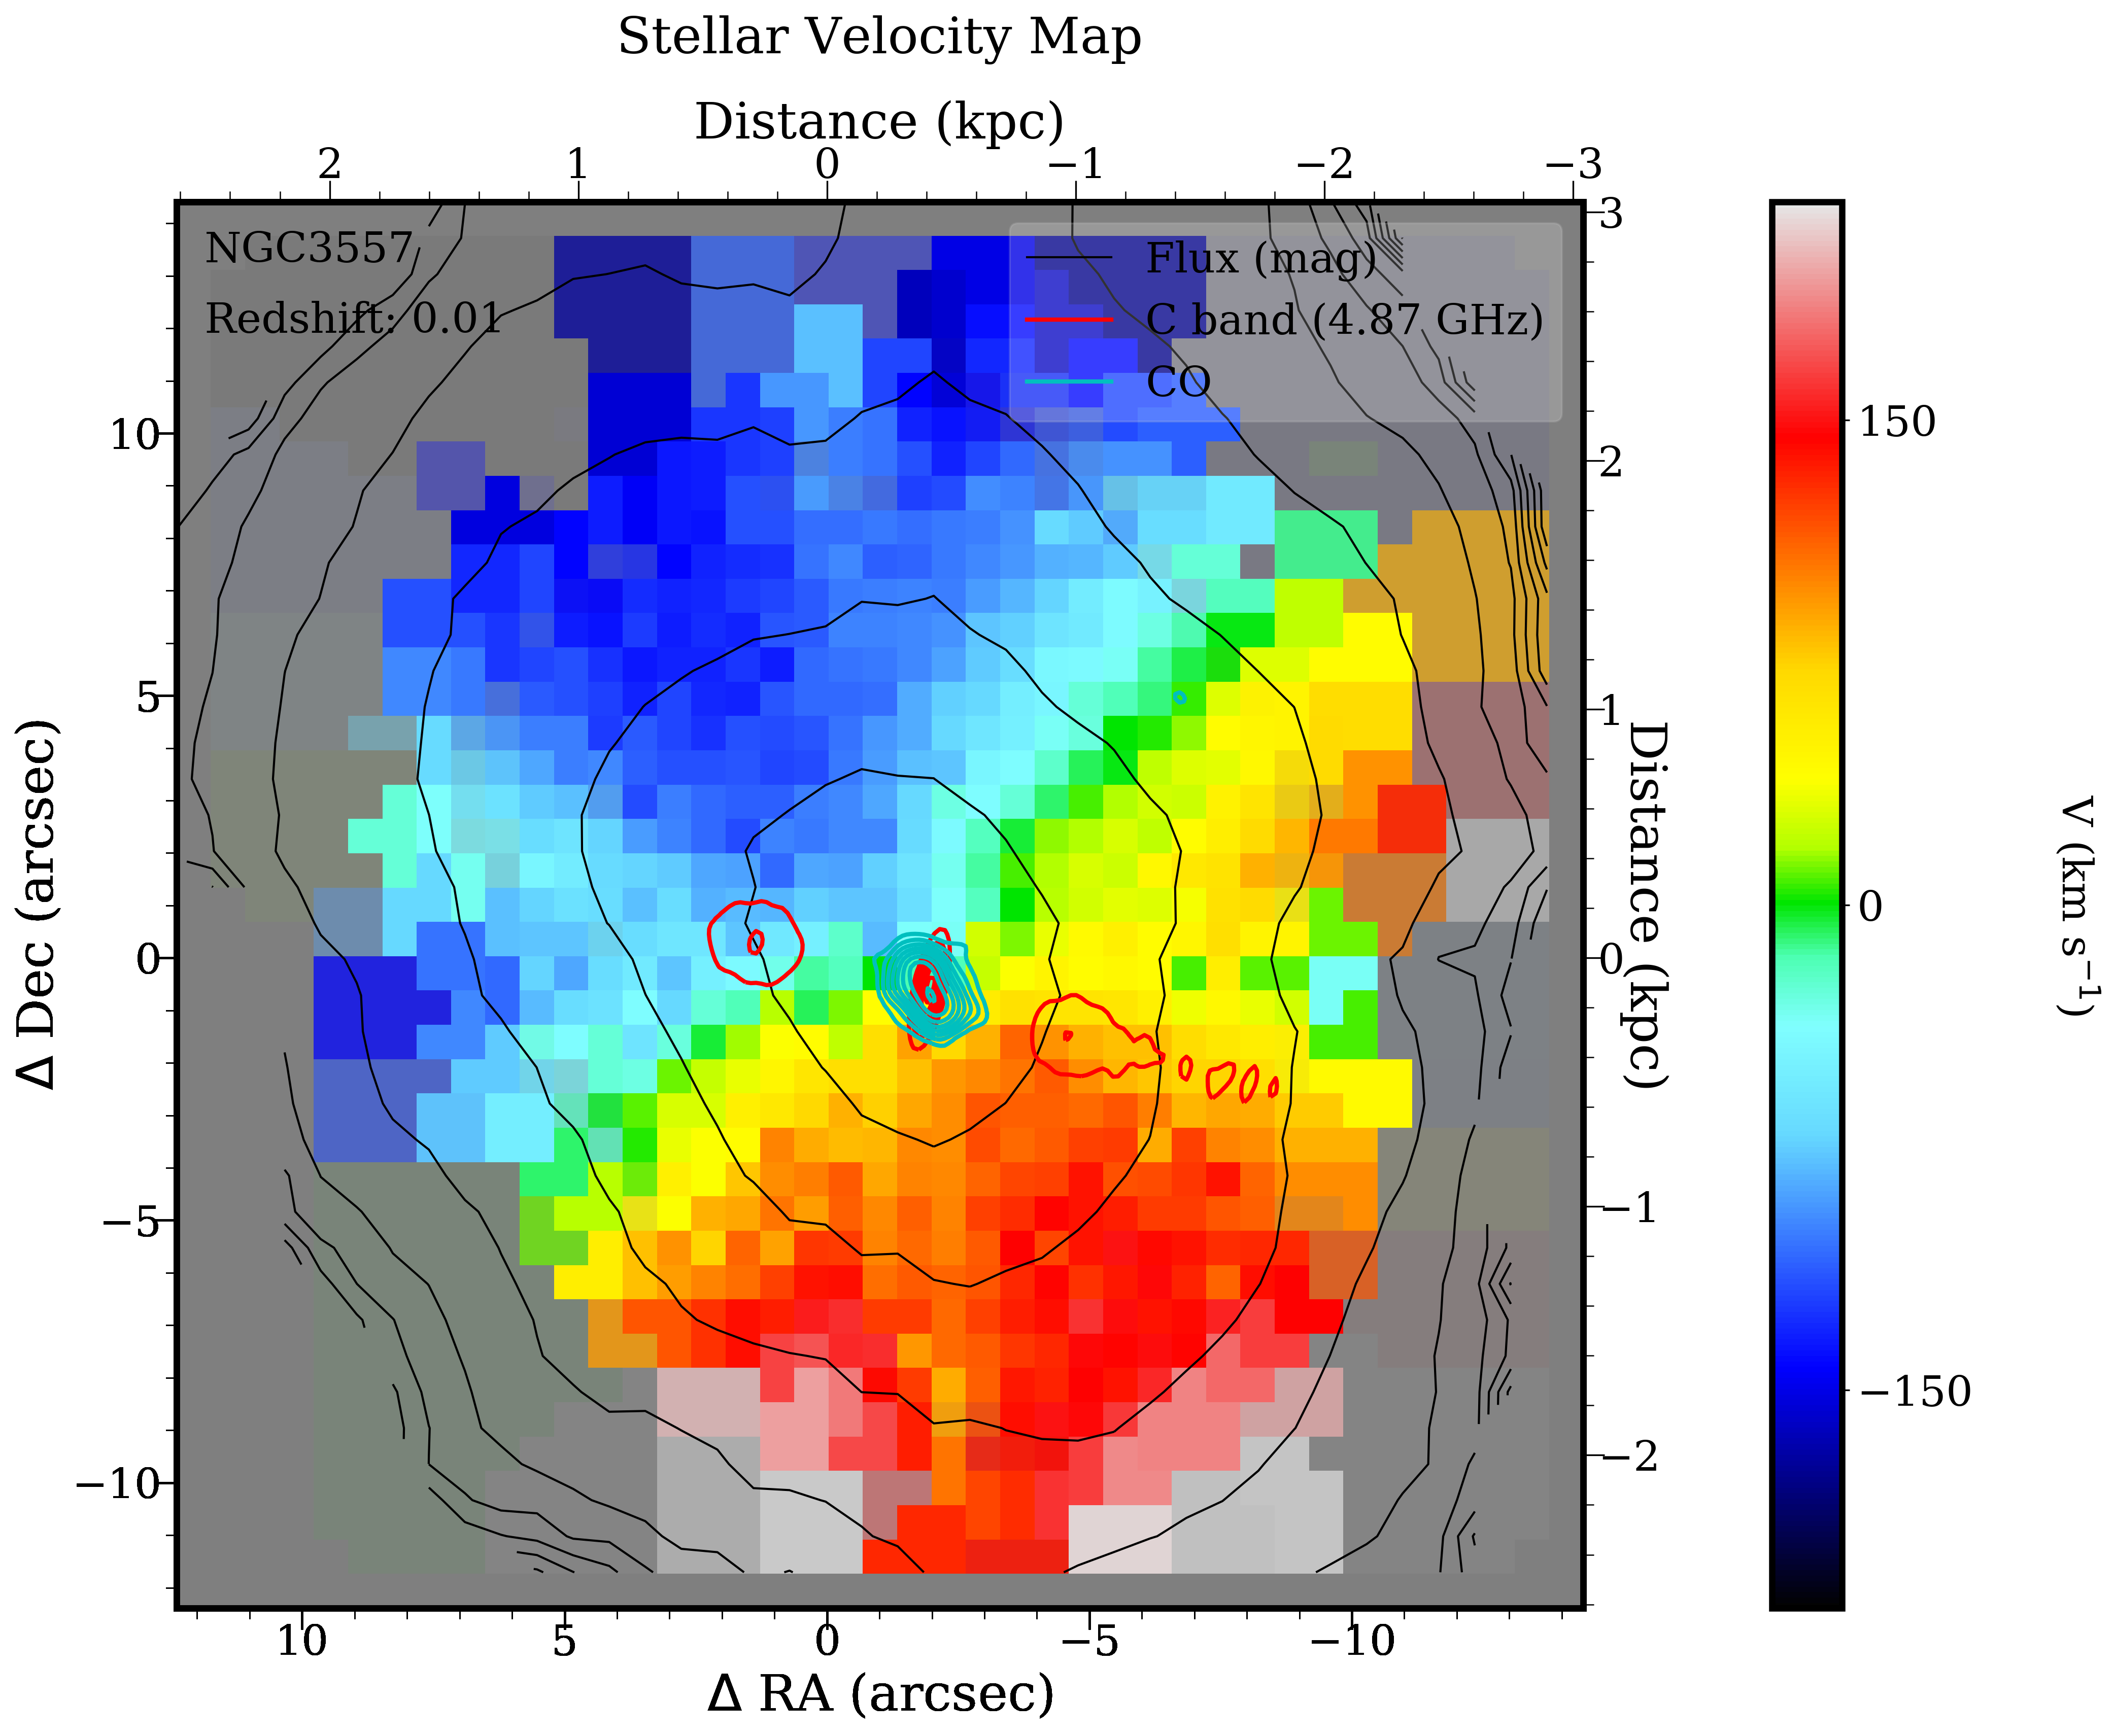
\includegraphics[width=0.245\textwidth]{Vmaps/ngc3557_stellar_vel.png}
      \includegraphics[width=0.245\textwidth]{Vmaps/ngc3100_stellar_vel.png}
      \includegraphics[width=0.245\textwidth]{Vmaps/ic1459_stellar_vel.png}
      \includegraphics[width=0.245\textwidth]{Vmaps/pks0718-34_stellar_vel.png}
      \includegraphics[width=0.245\textwidth]{Vmaps/ic4296_stellar_vel.png}
      \includegraphics[width=0.245\textwidth]{Vmaps/ngc7075_stellar_vel.png}
      \includegraphics[width=0.245\textwidth]{Vmaps/ic1531_stellar_vel.png}
      \includegraphics[width=0.245\textwidth]{Vmaps/ngc1399_stellar_vel.png}
      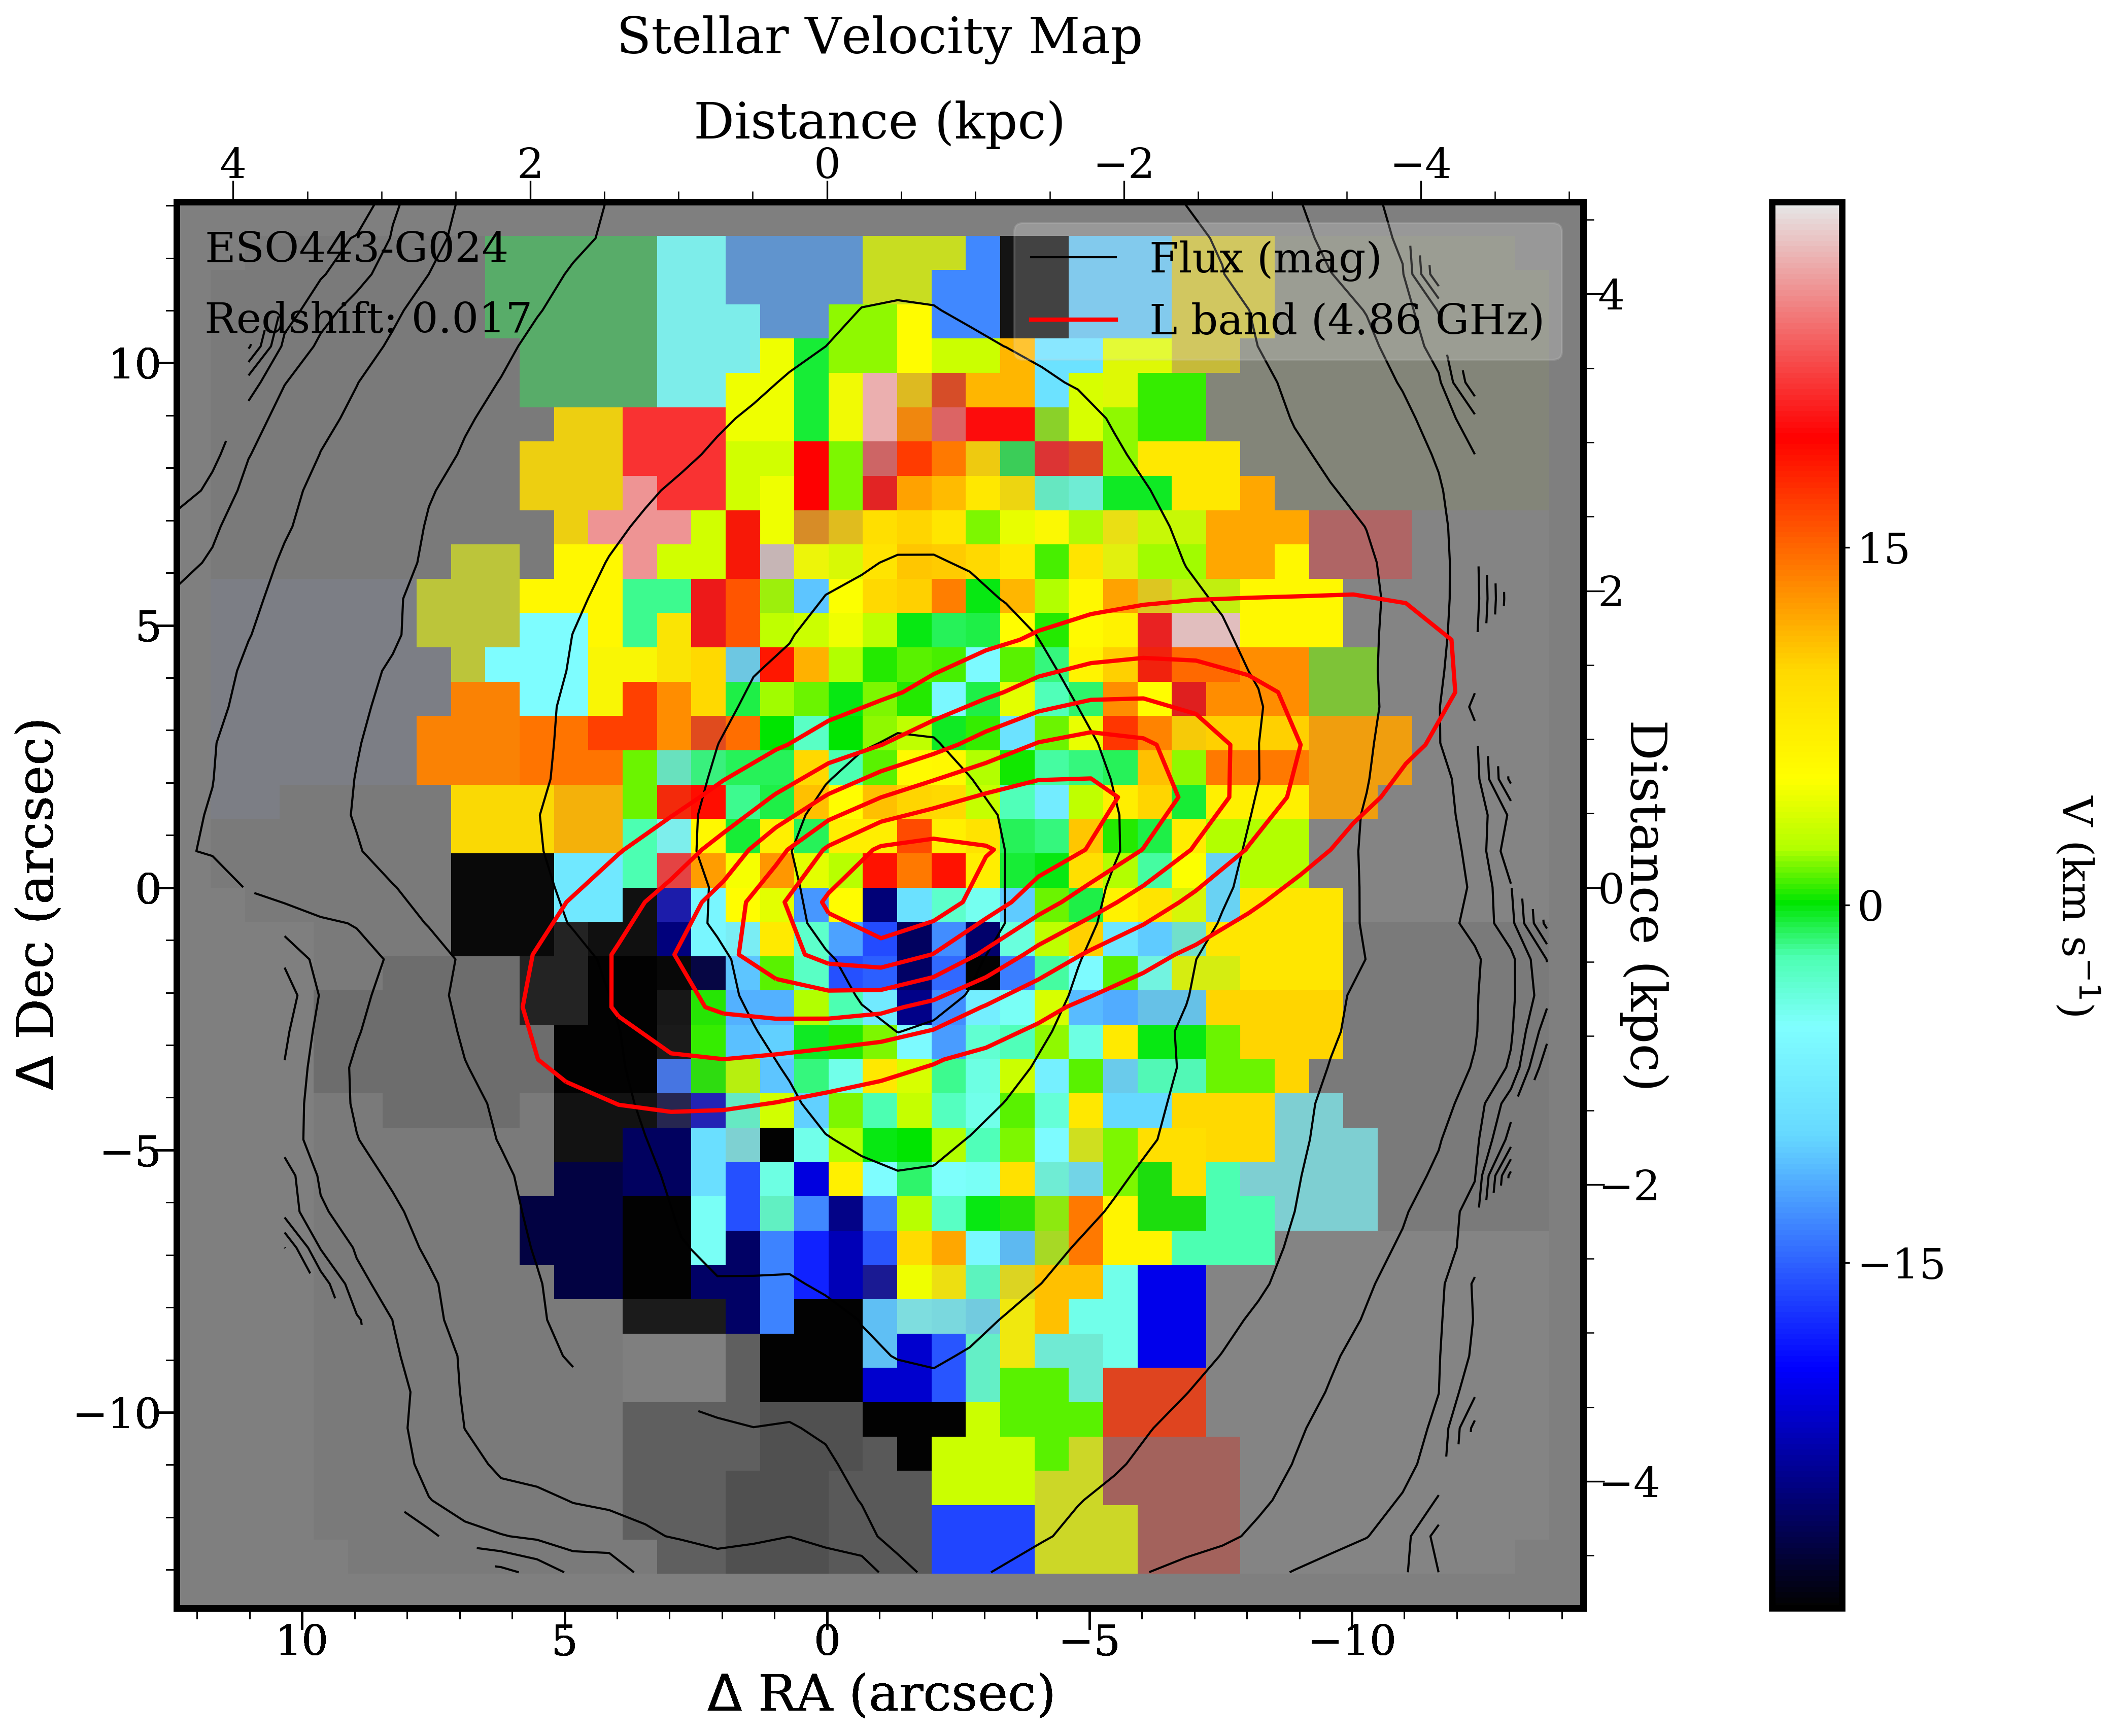
\includegraphics[width=0.245\textwidth]{Vmaps/eso443-g024_stellar_vel.png}
      \caption[VIMOS velocity maps]{Velocity for each galaxy in the VIMOS sample. Plots are ordered and contour colors are as in figure \ref{fig:Vstellar_img}}
      \label{fig:Vstellar_vel}
\end{figure*}

\begin{figure*}
      \centering
      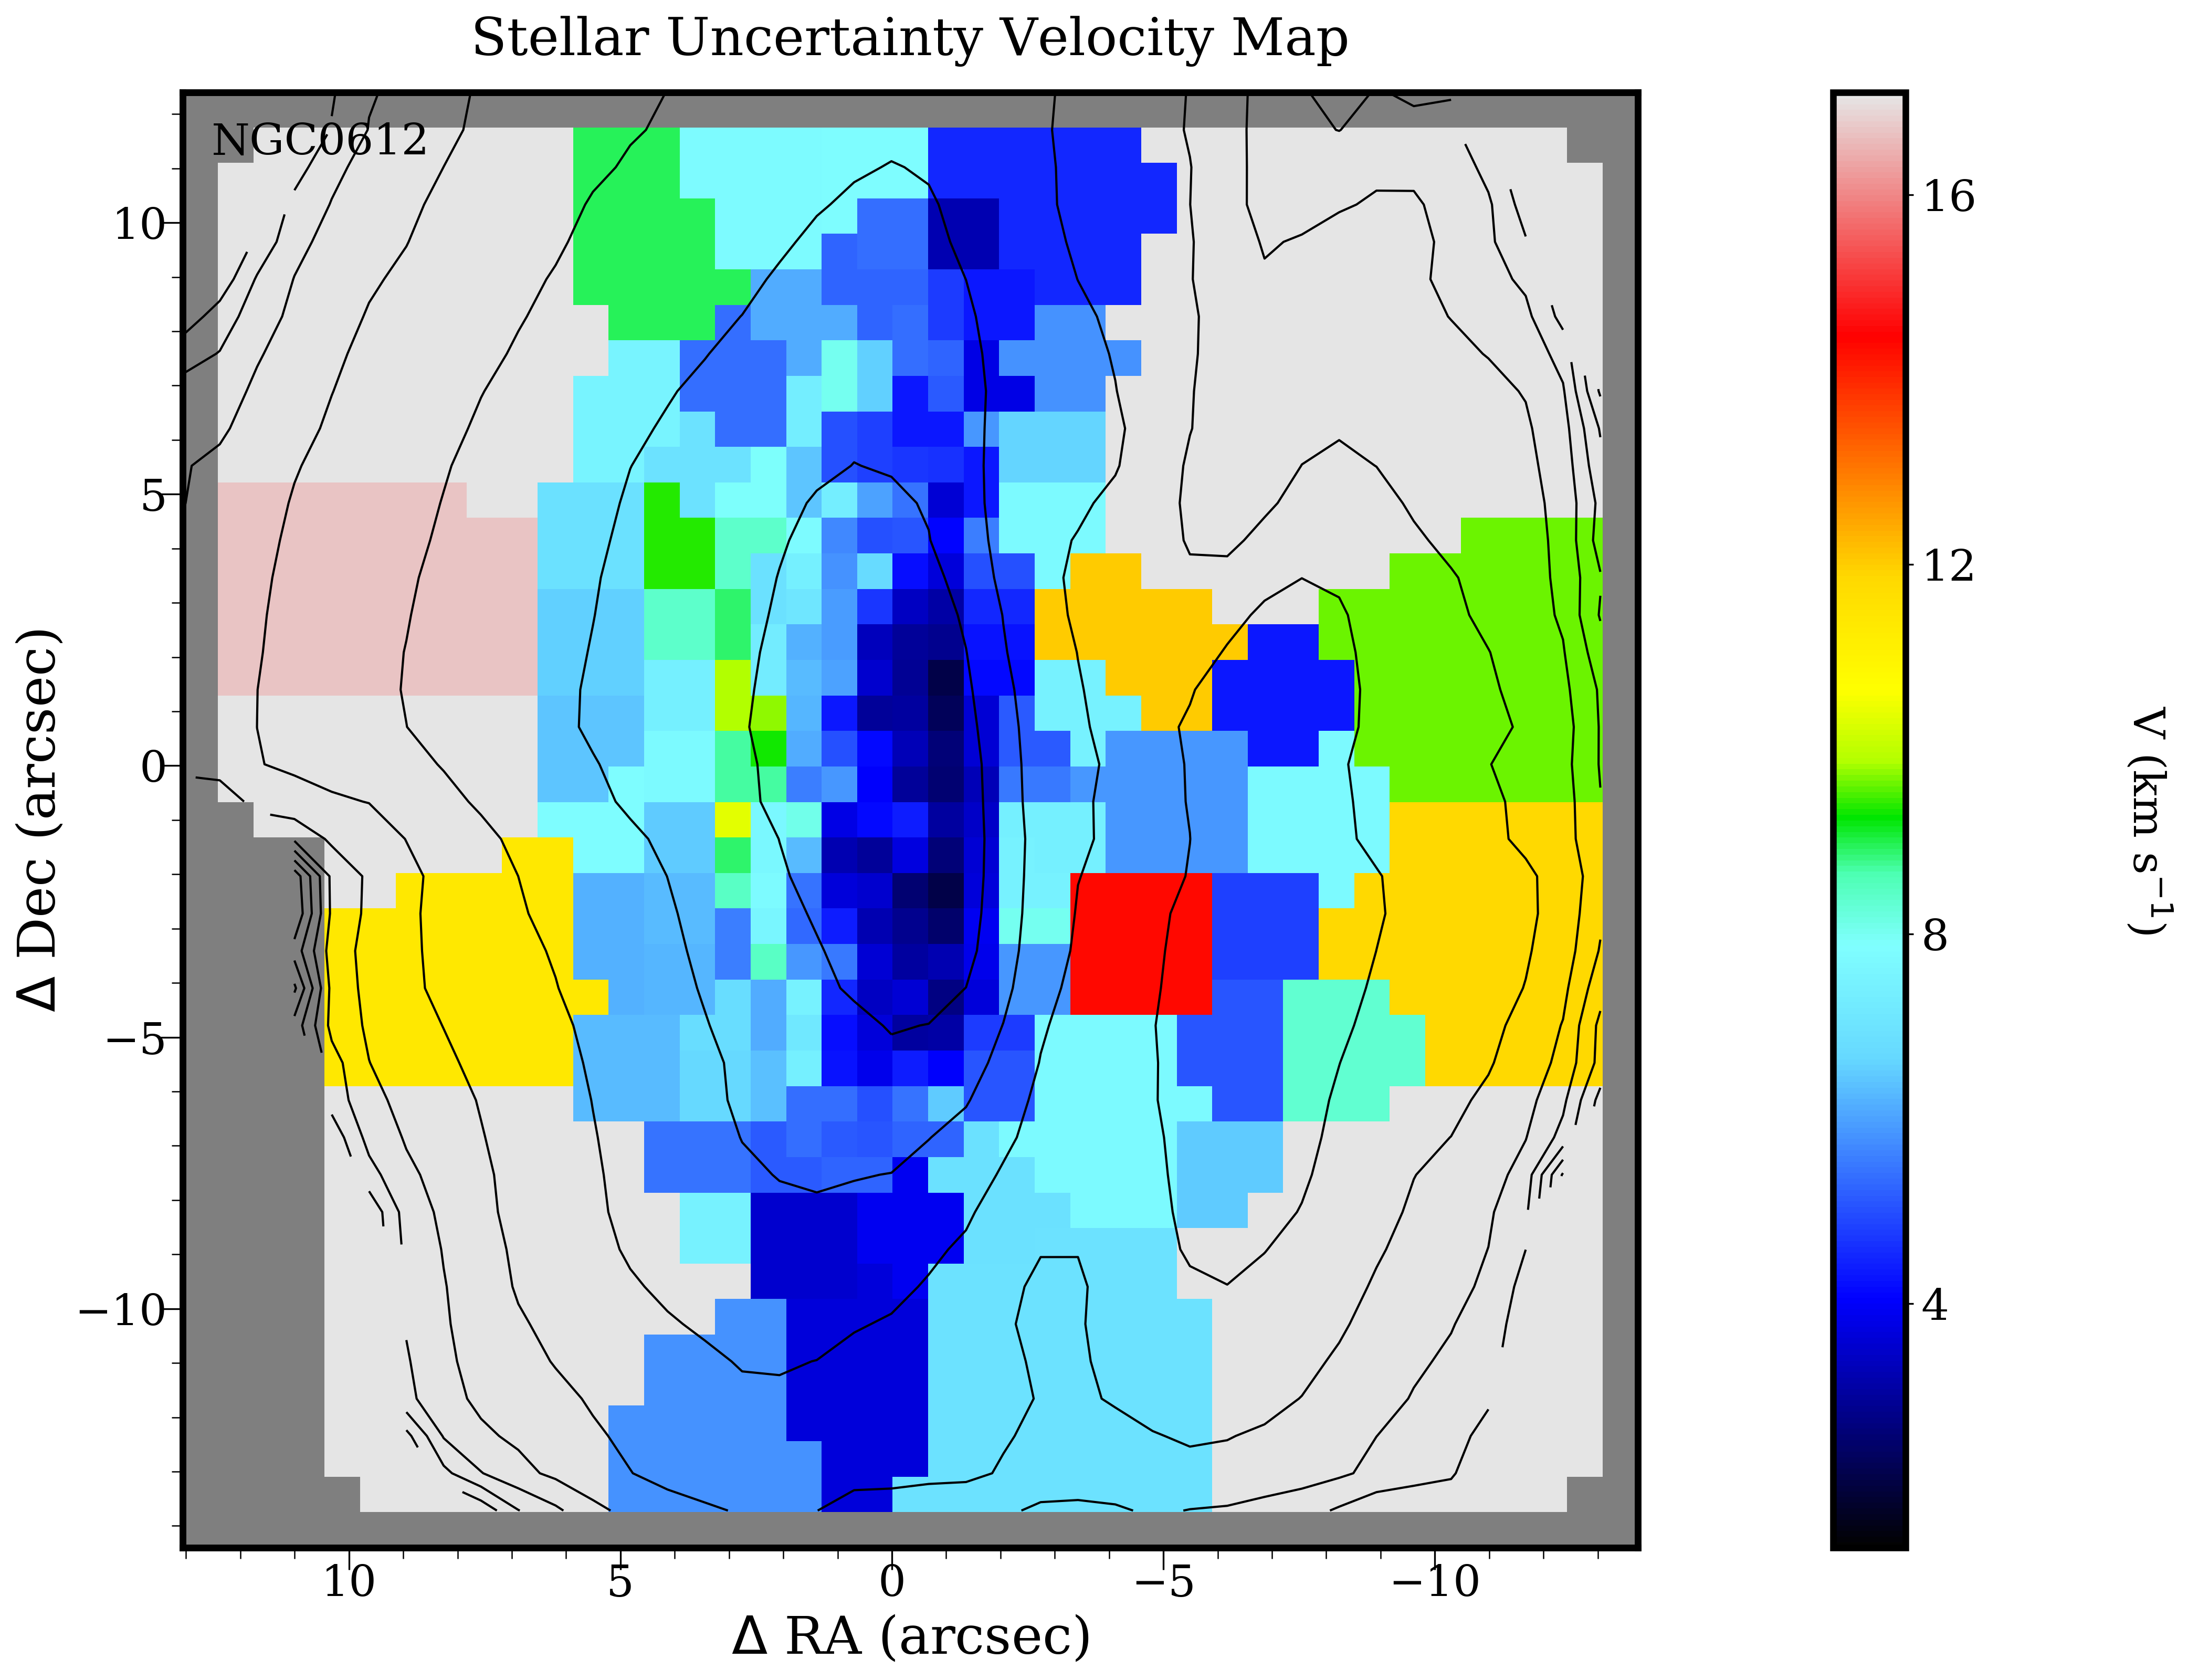
\includegraphics[width=0.245\textwidth]{Vmaps/ngc0612_stellar_vel_uncert.png}
      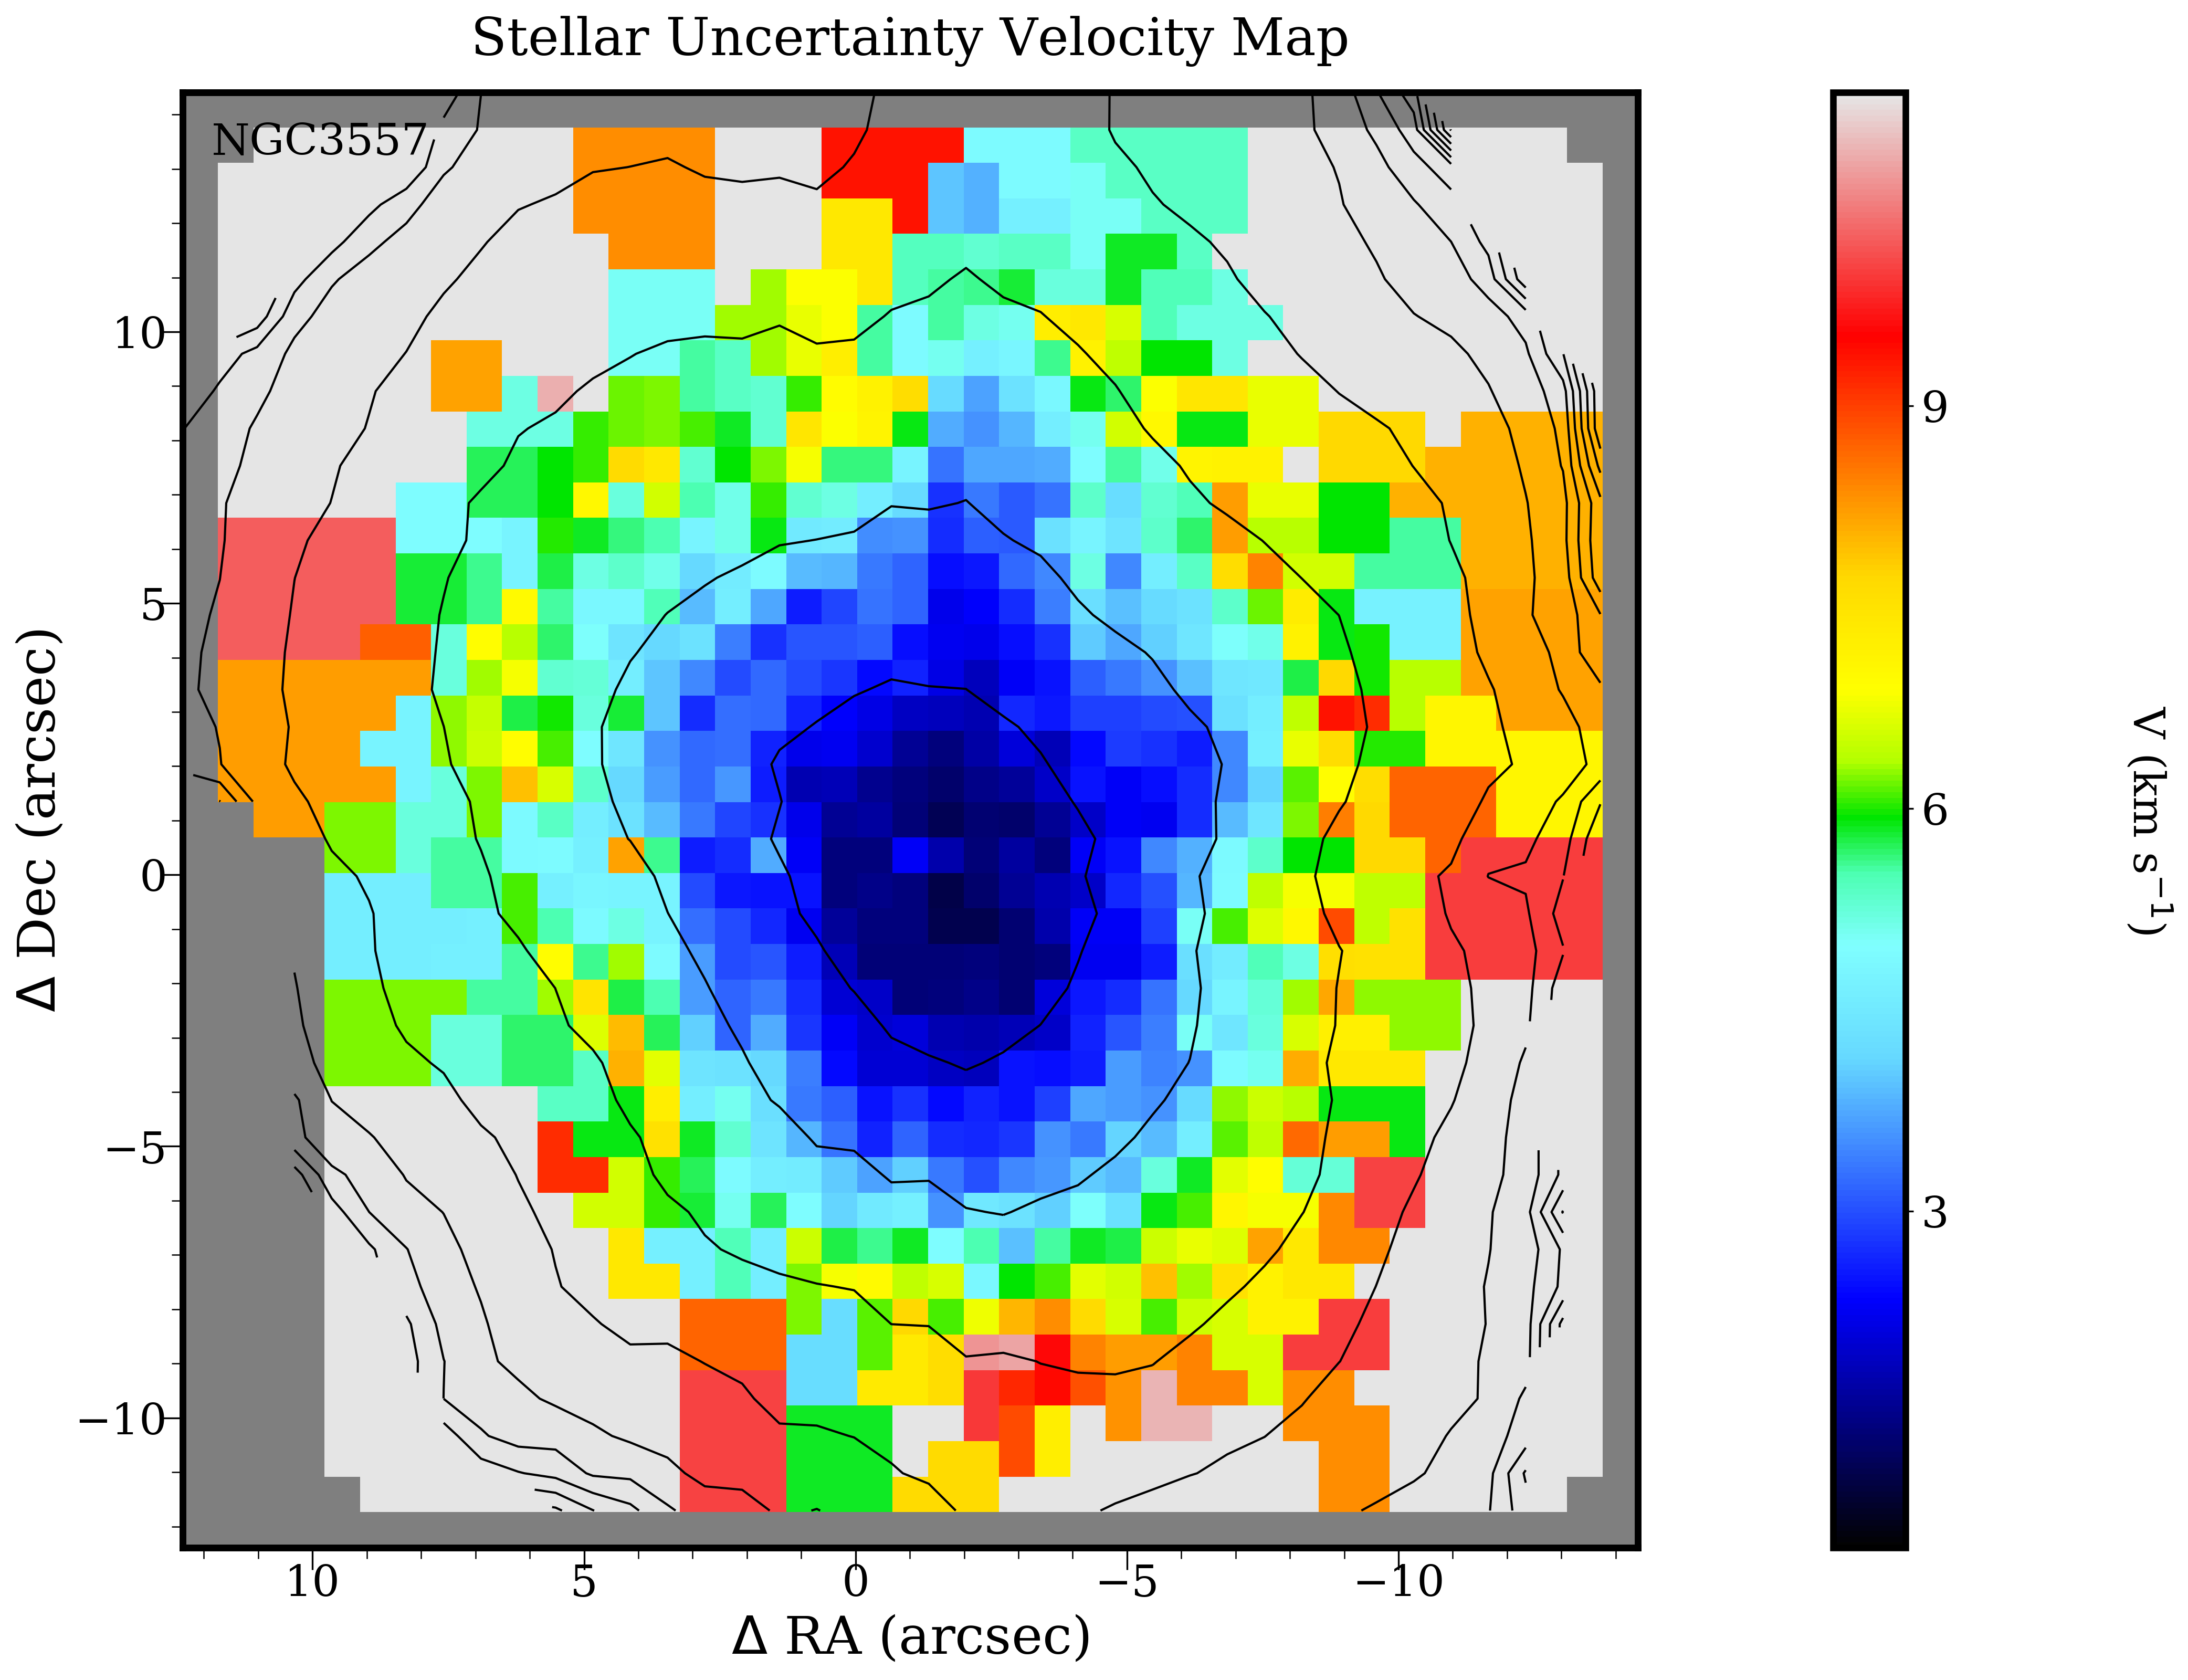
\includegraphics[width=0.245\textwidth]{Vmaps/ngc3557_stellar_vel_uncert.png}
      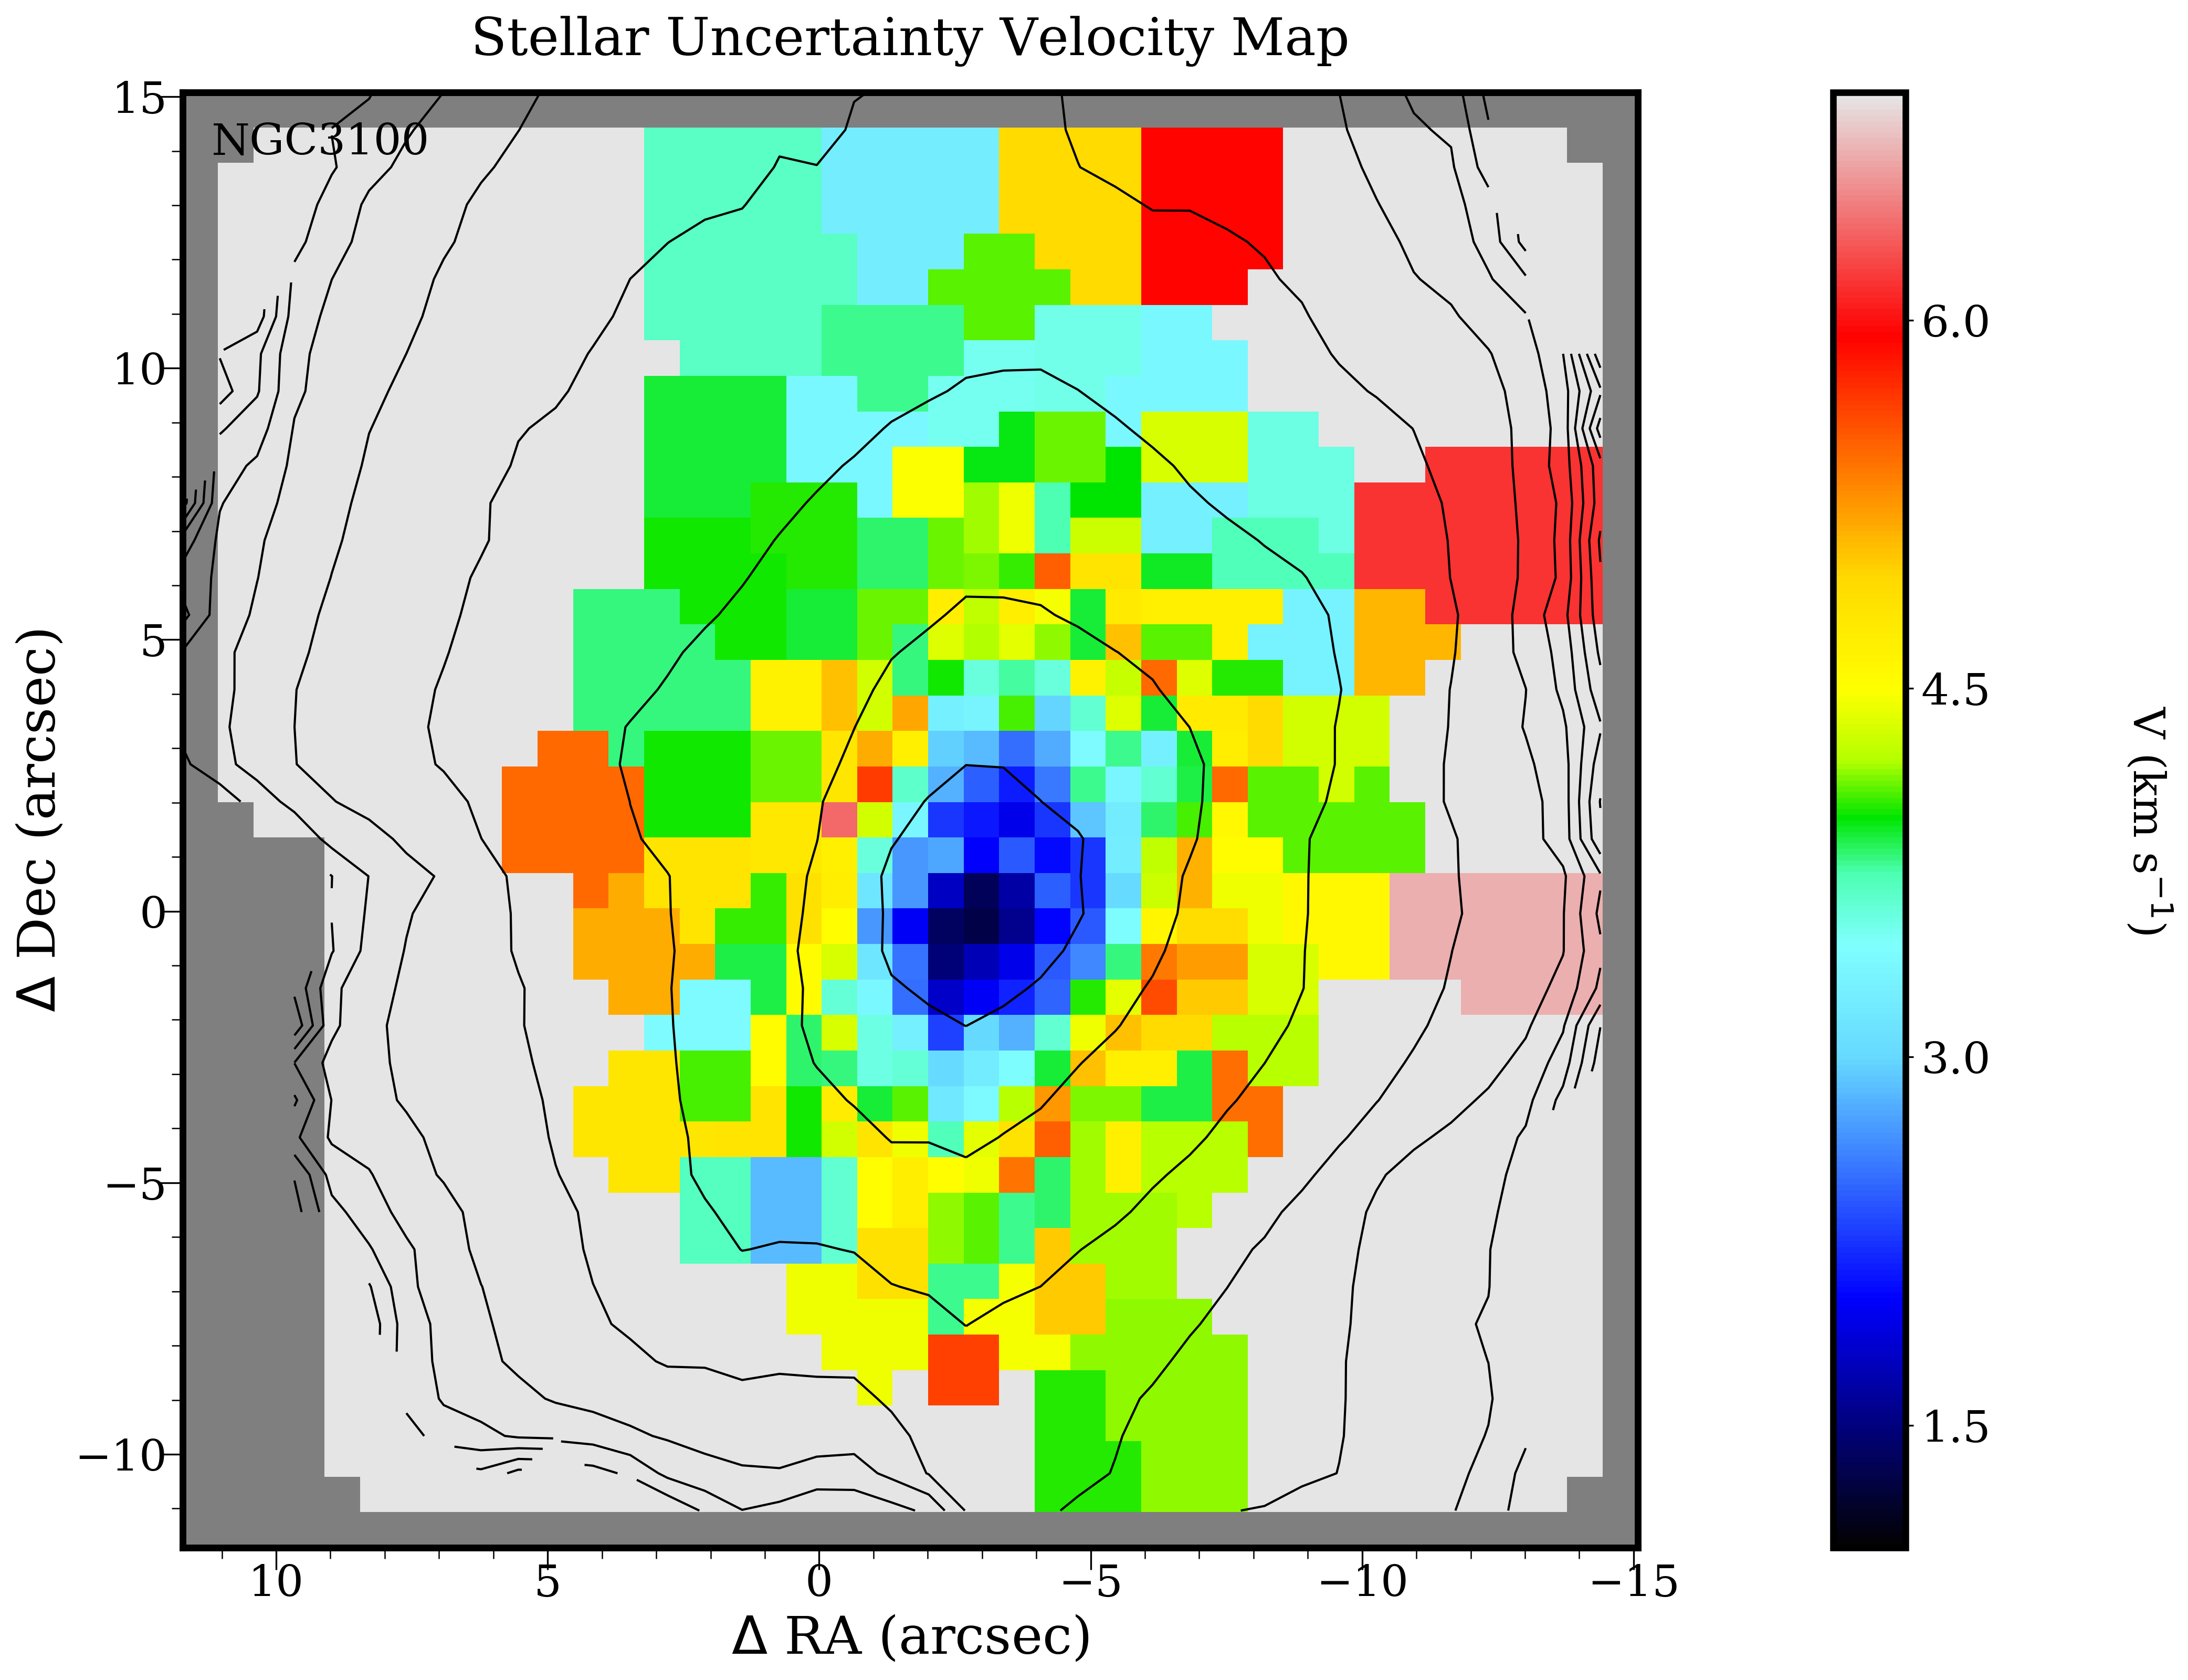
\includegraphics[width=0.245\textwidth]{Vmaps/ngc3100_stellar_vel_uncert.png}
      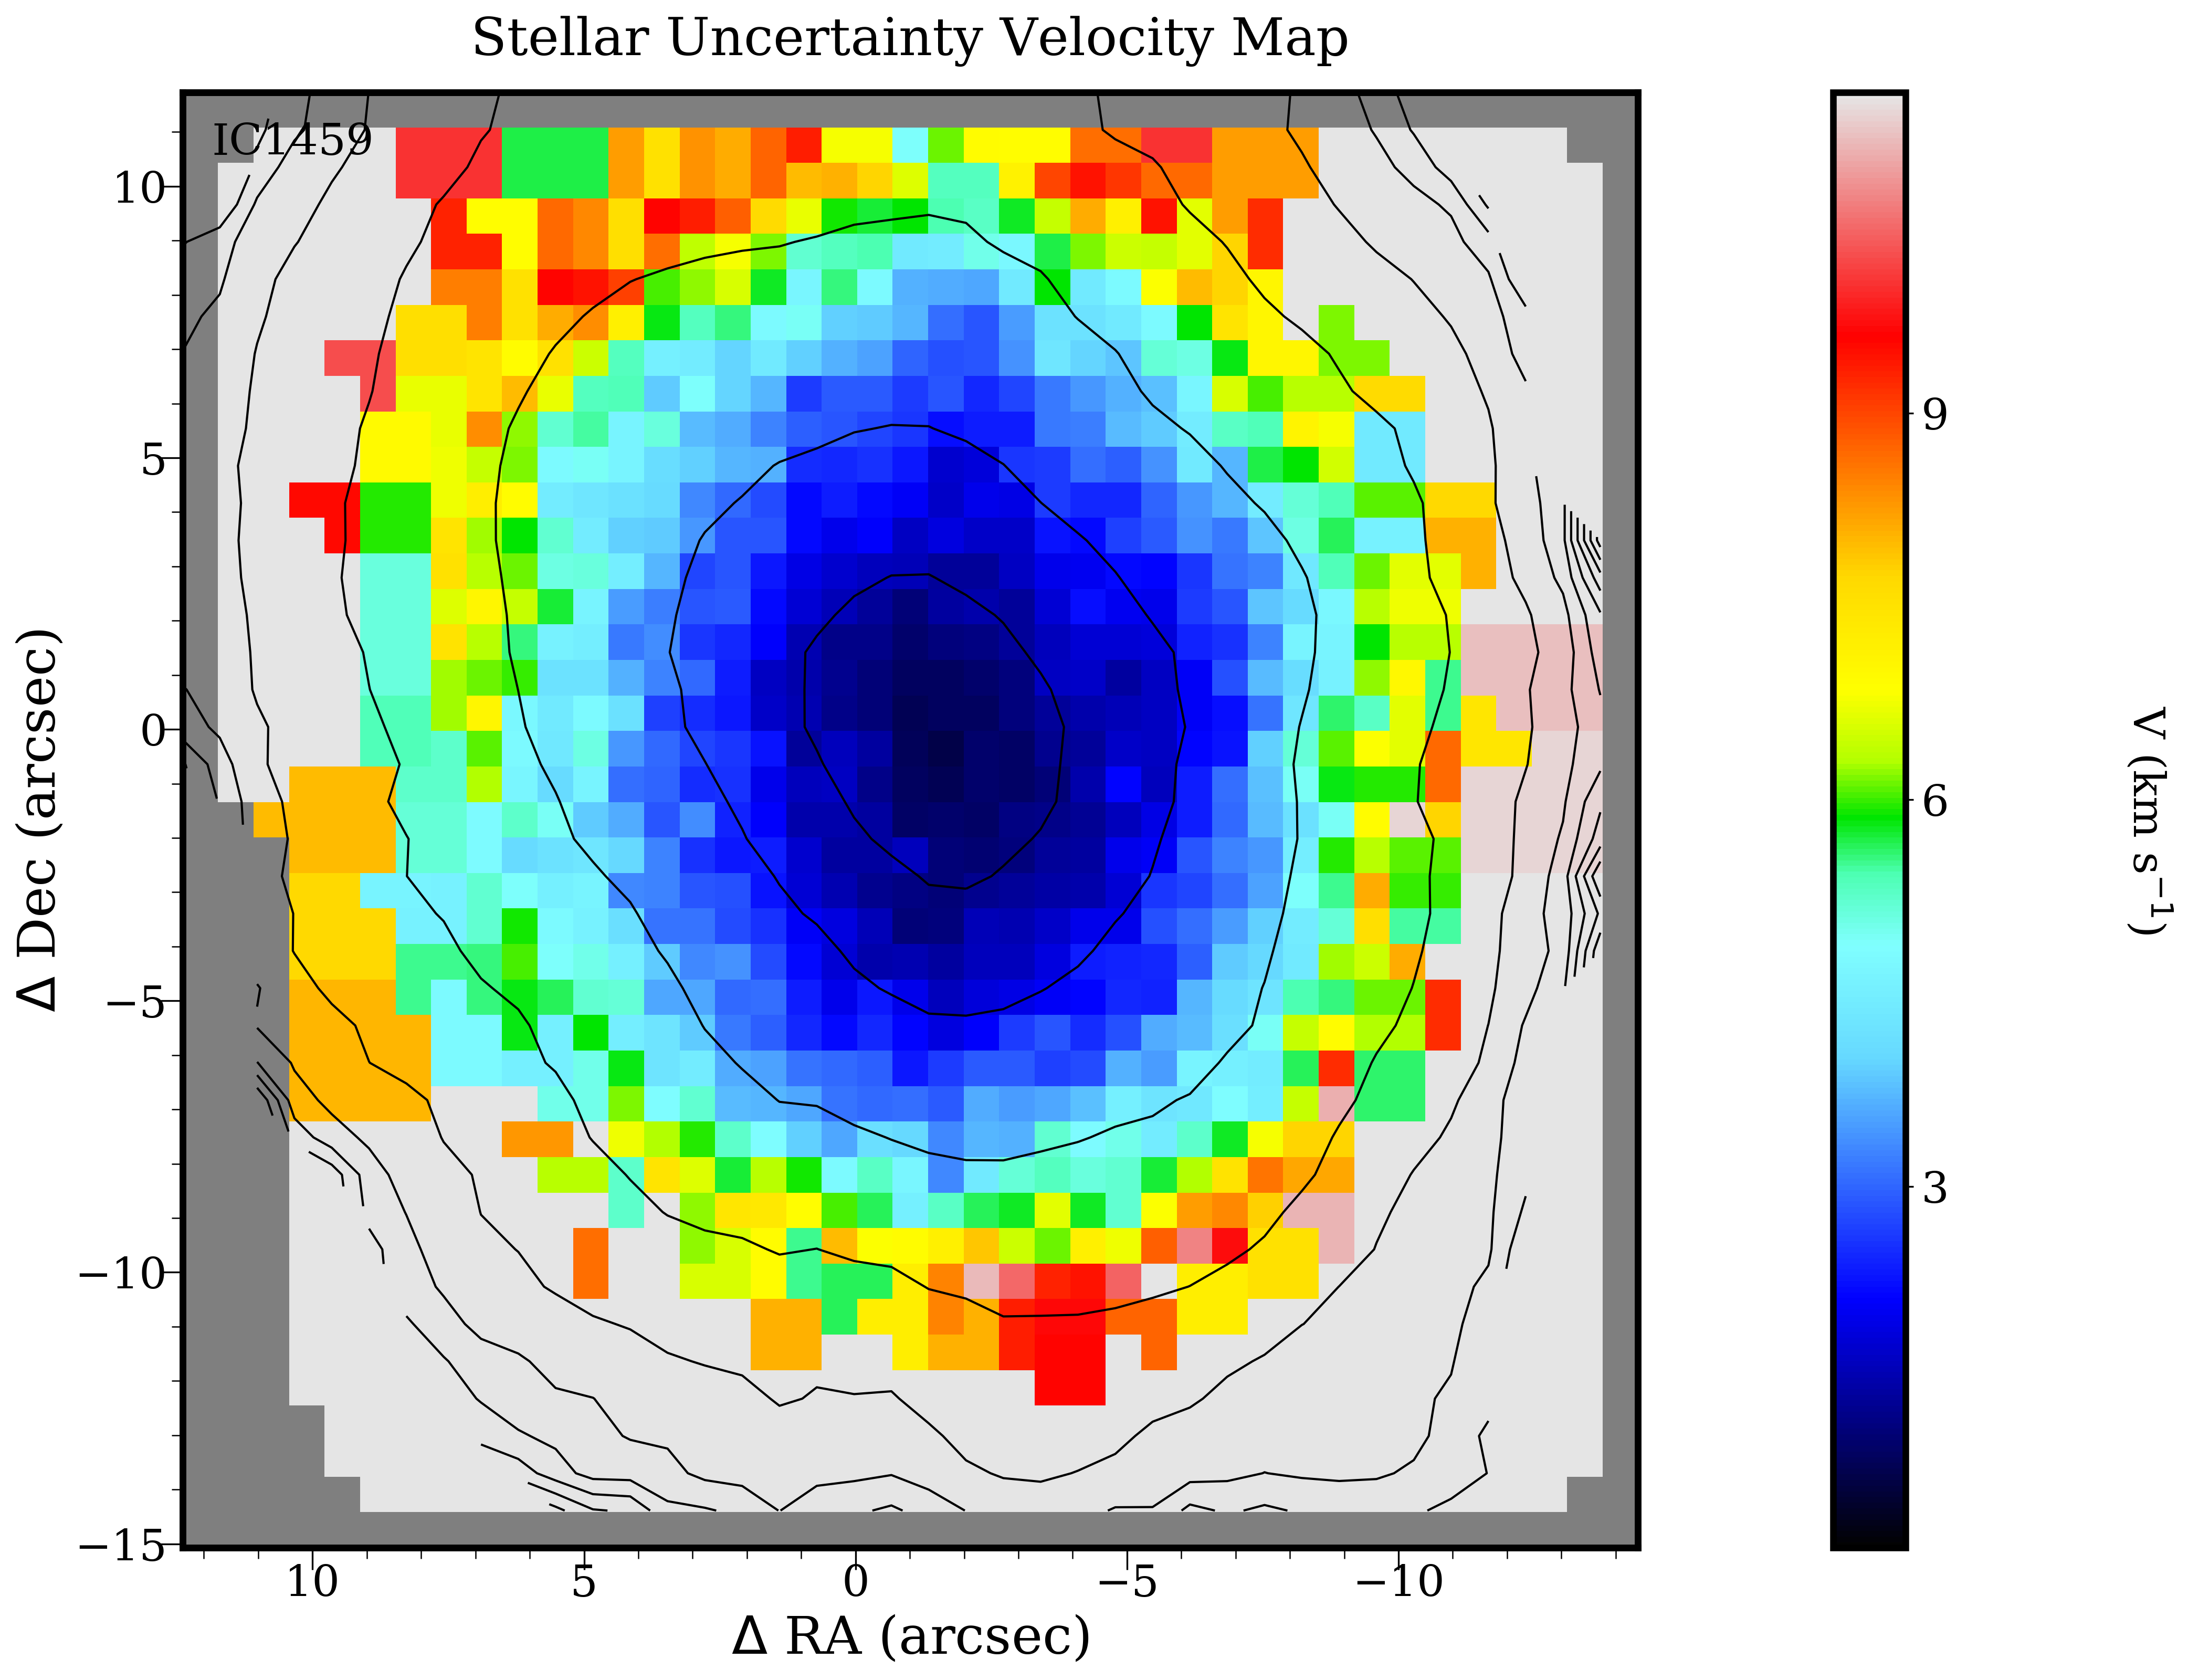
\includegraphics[width=0.245\textwidth]{Vmaps/ic1459_stellar_vel_uncert.png}
      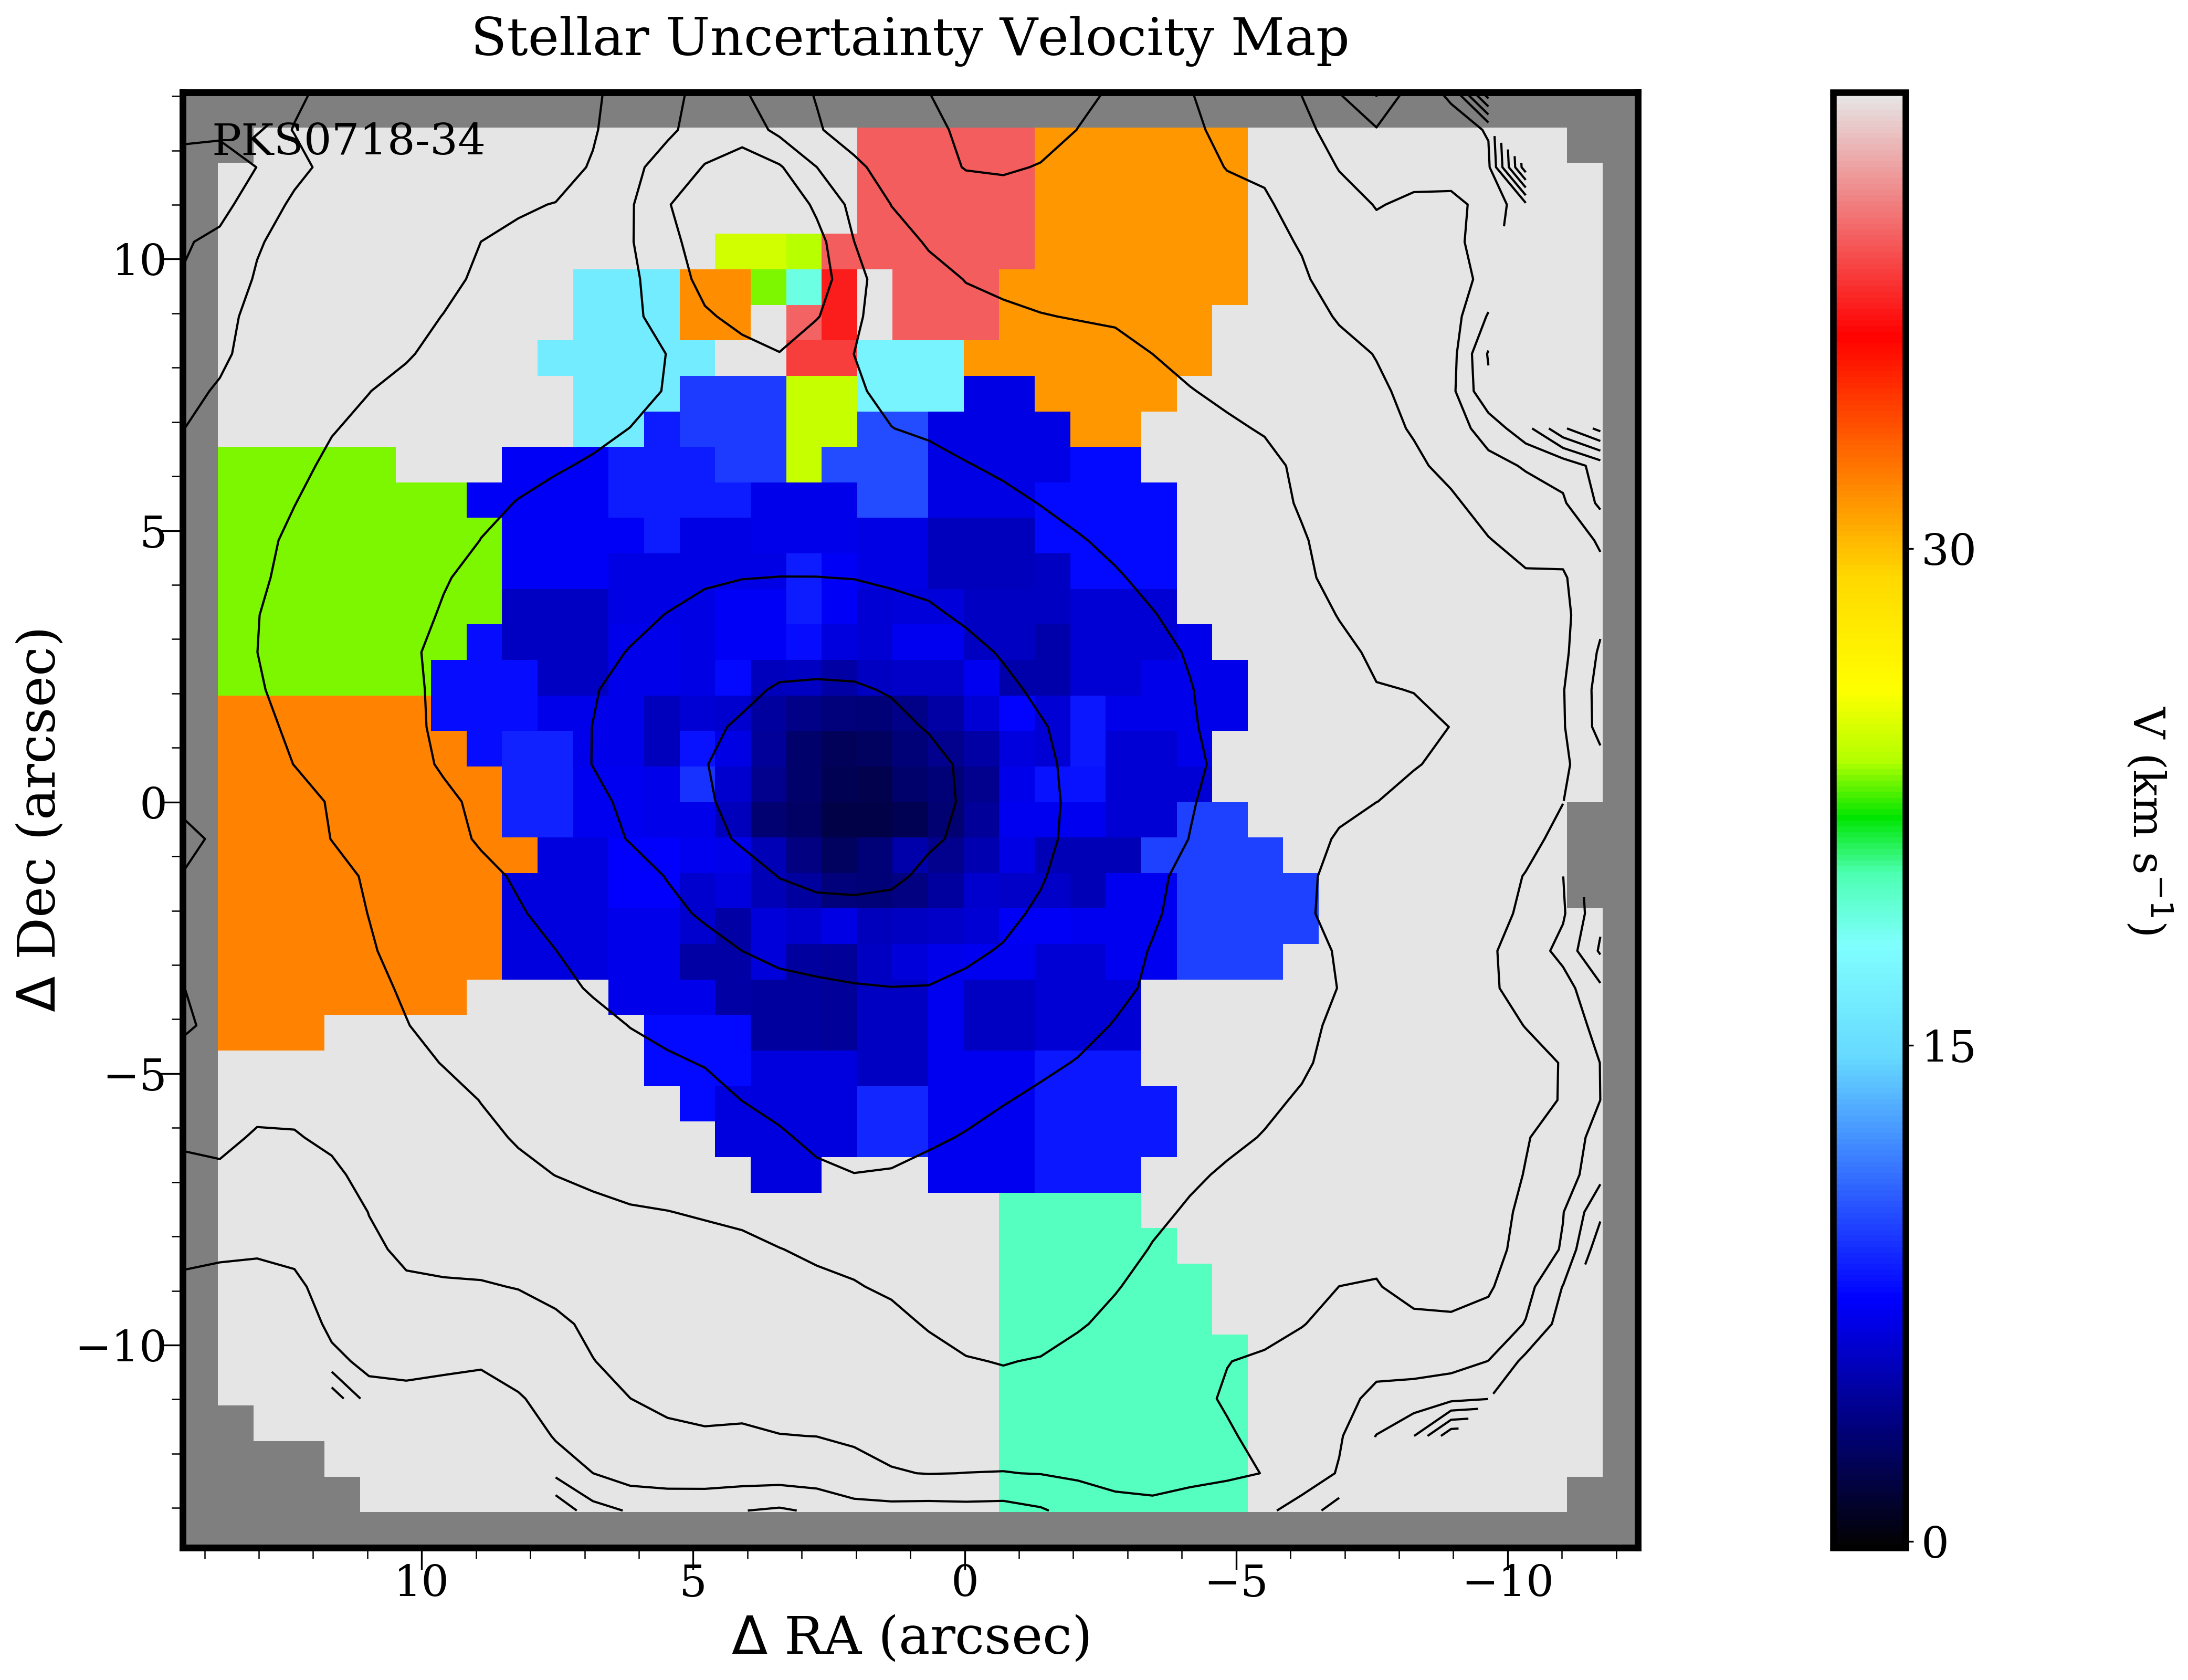
\includegraphics[width=0.245\textwidth]{Vmaps/pks0718-34_stellar_vel_uncert.png}
      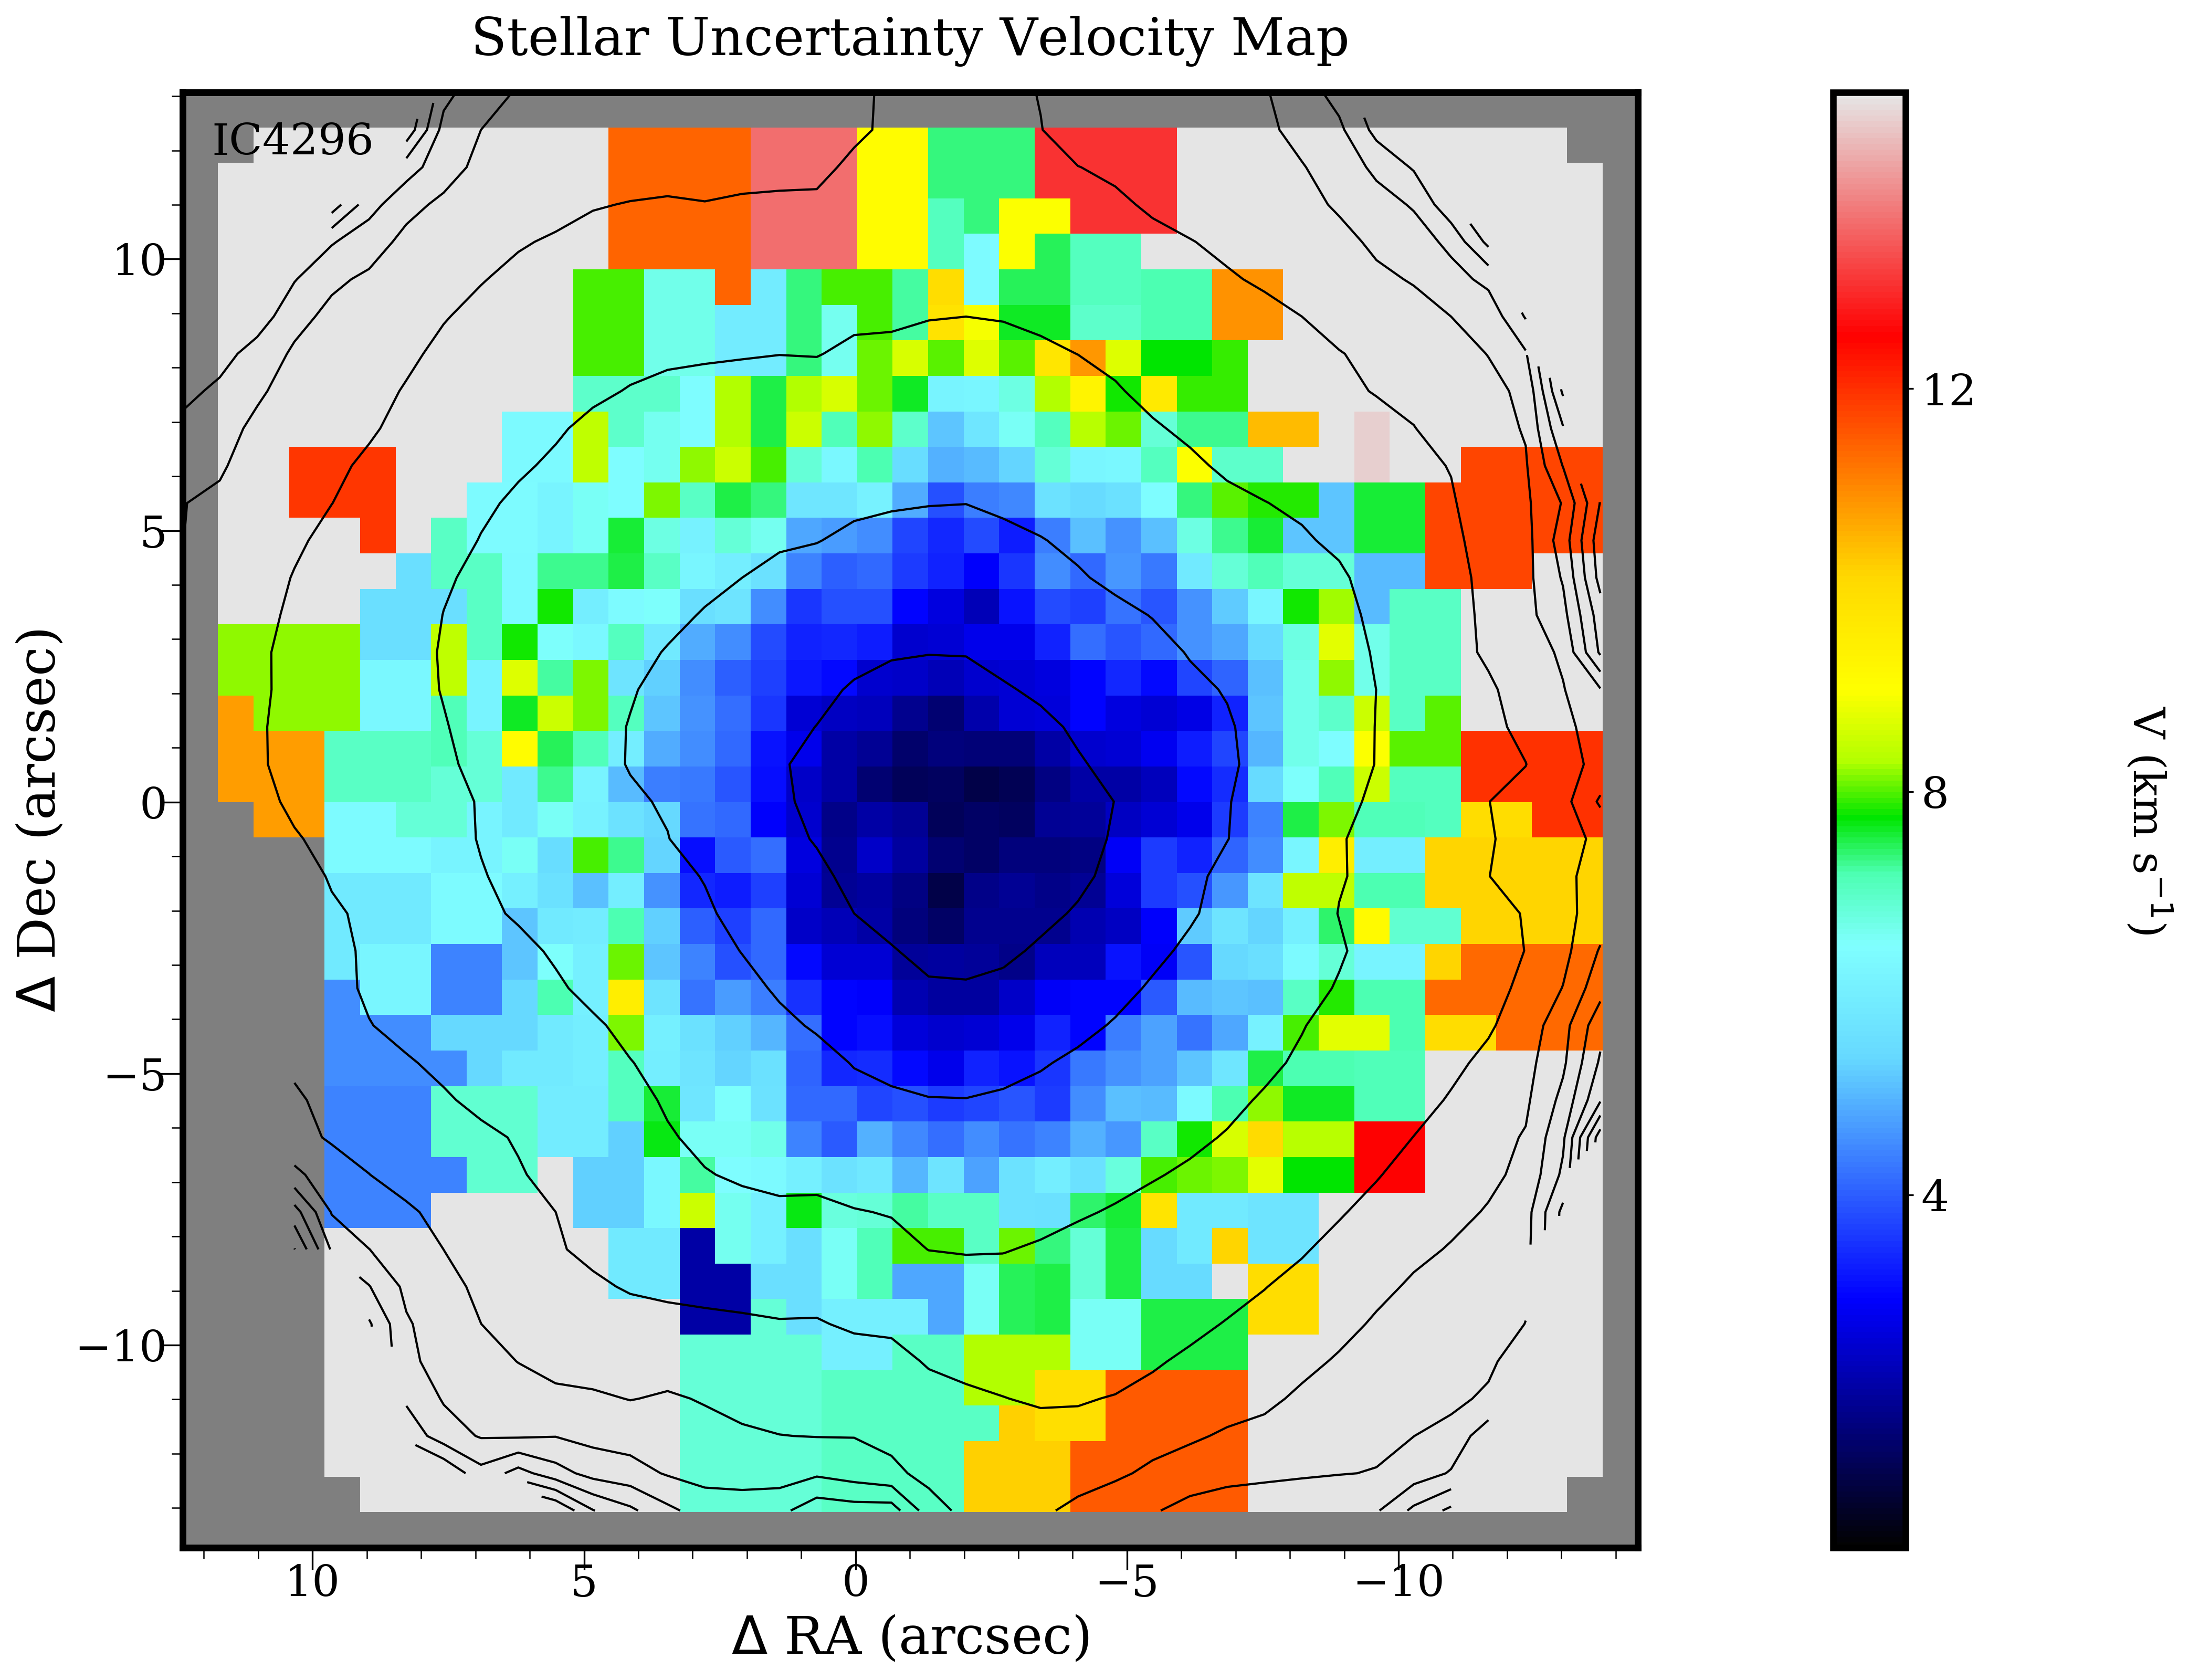
\includegraphics[width=0.245\textwidth]{Vmaps/ic4296_stellar_vel_uncert.png}
      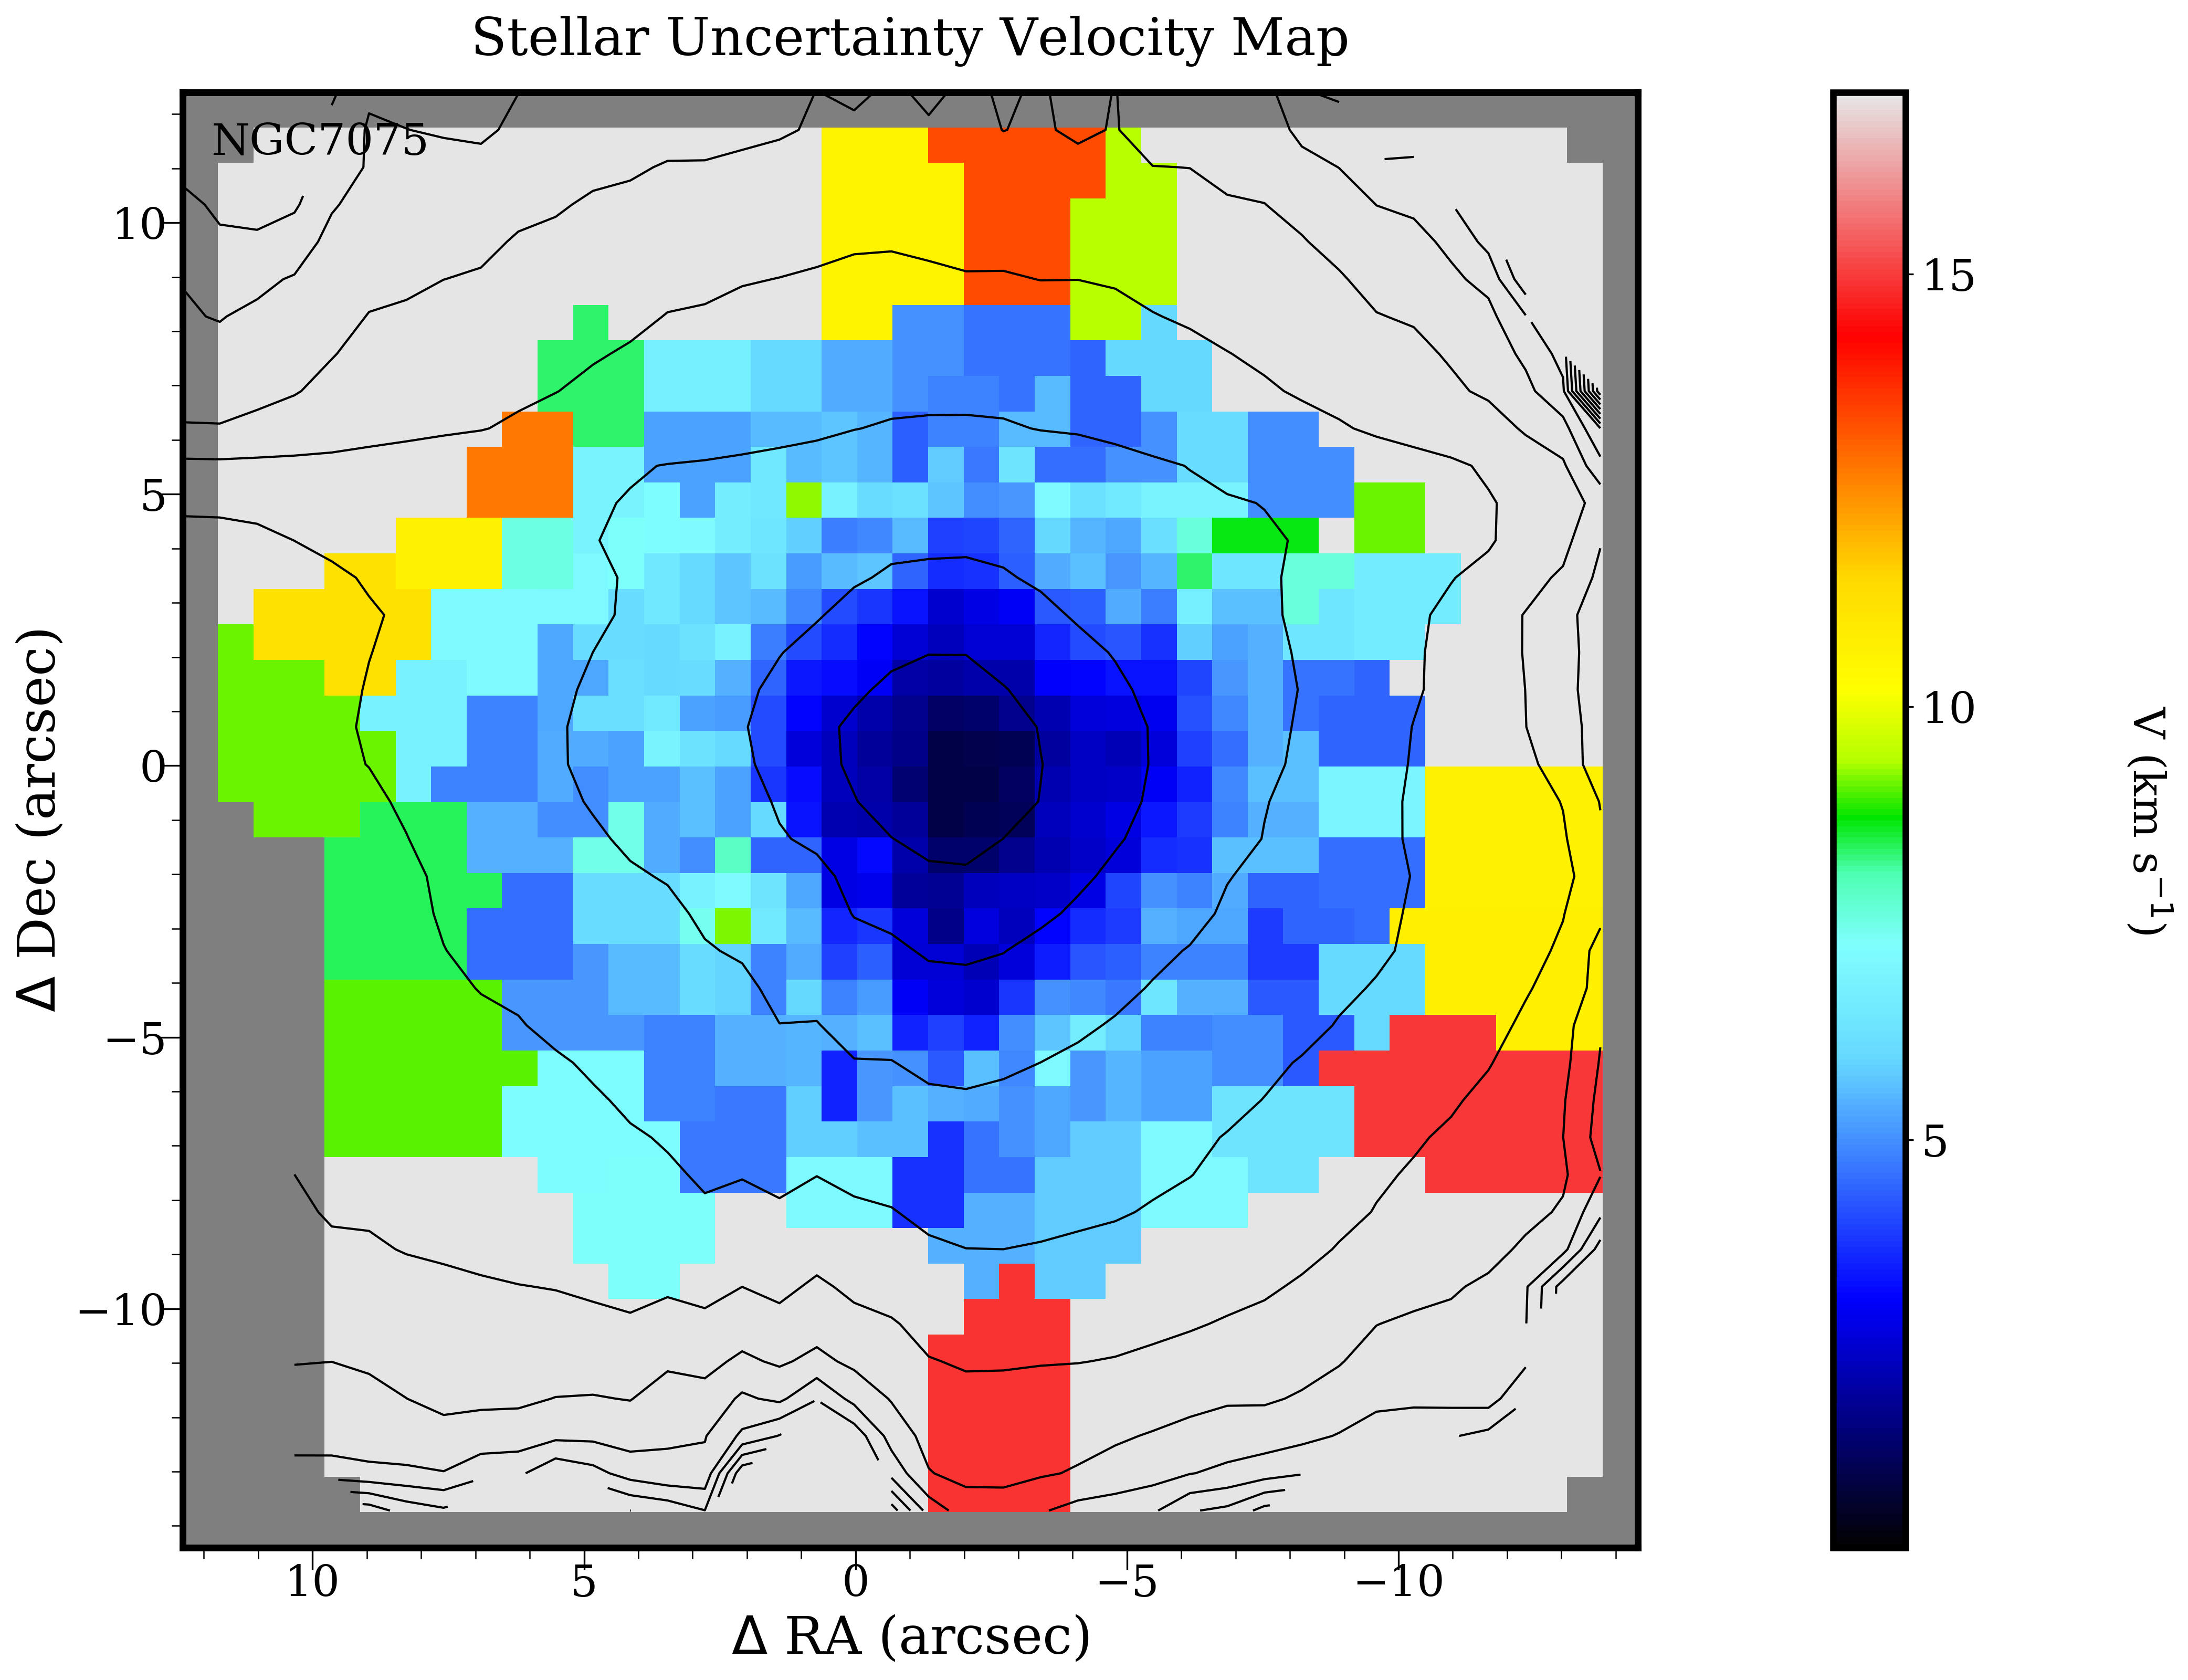
\includegraphics[width=0.245\textwidth]{Vmaps/ngc7075_stellar_vel_uncert.png}
      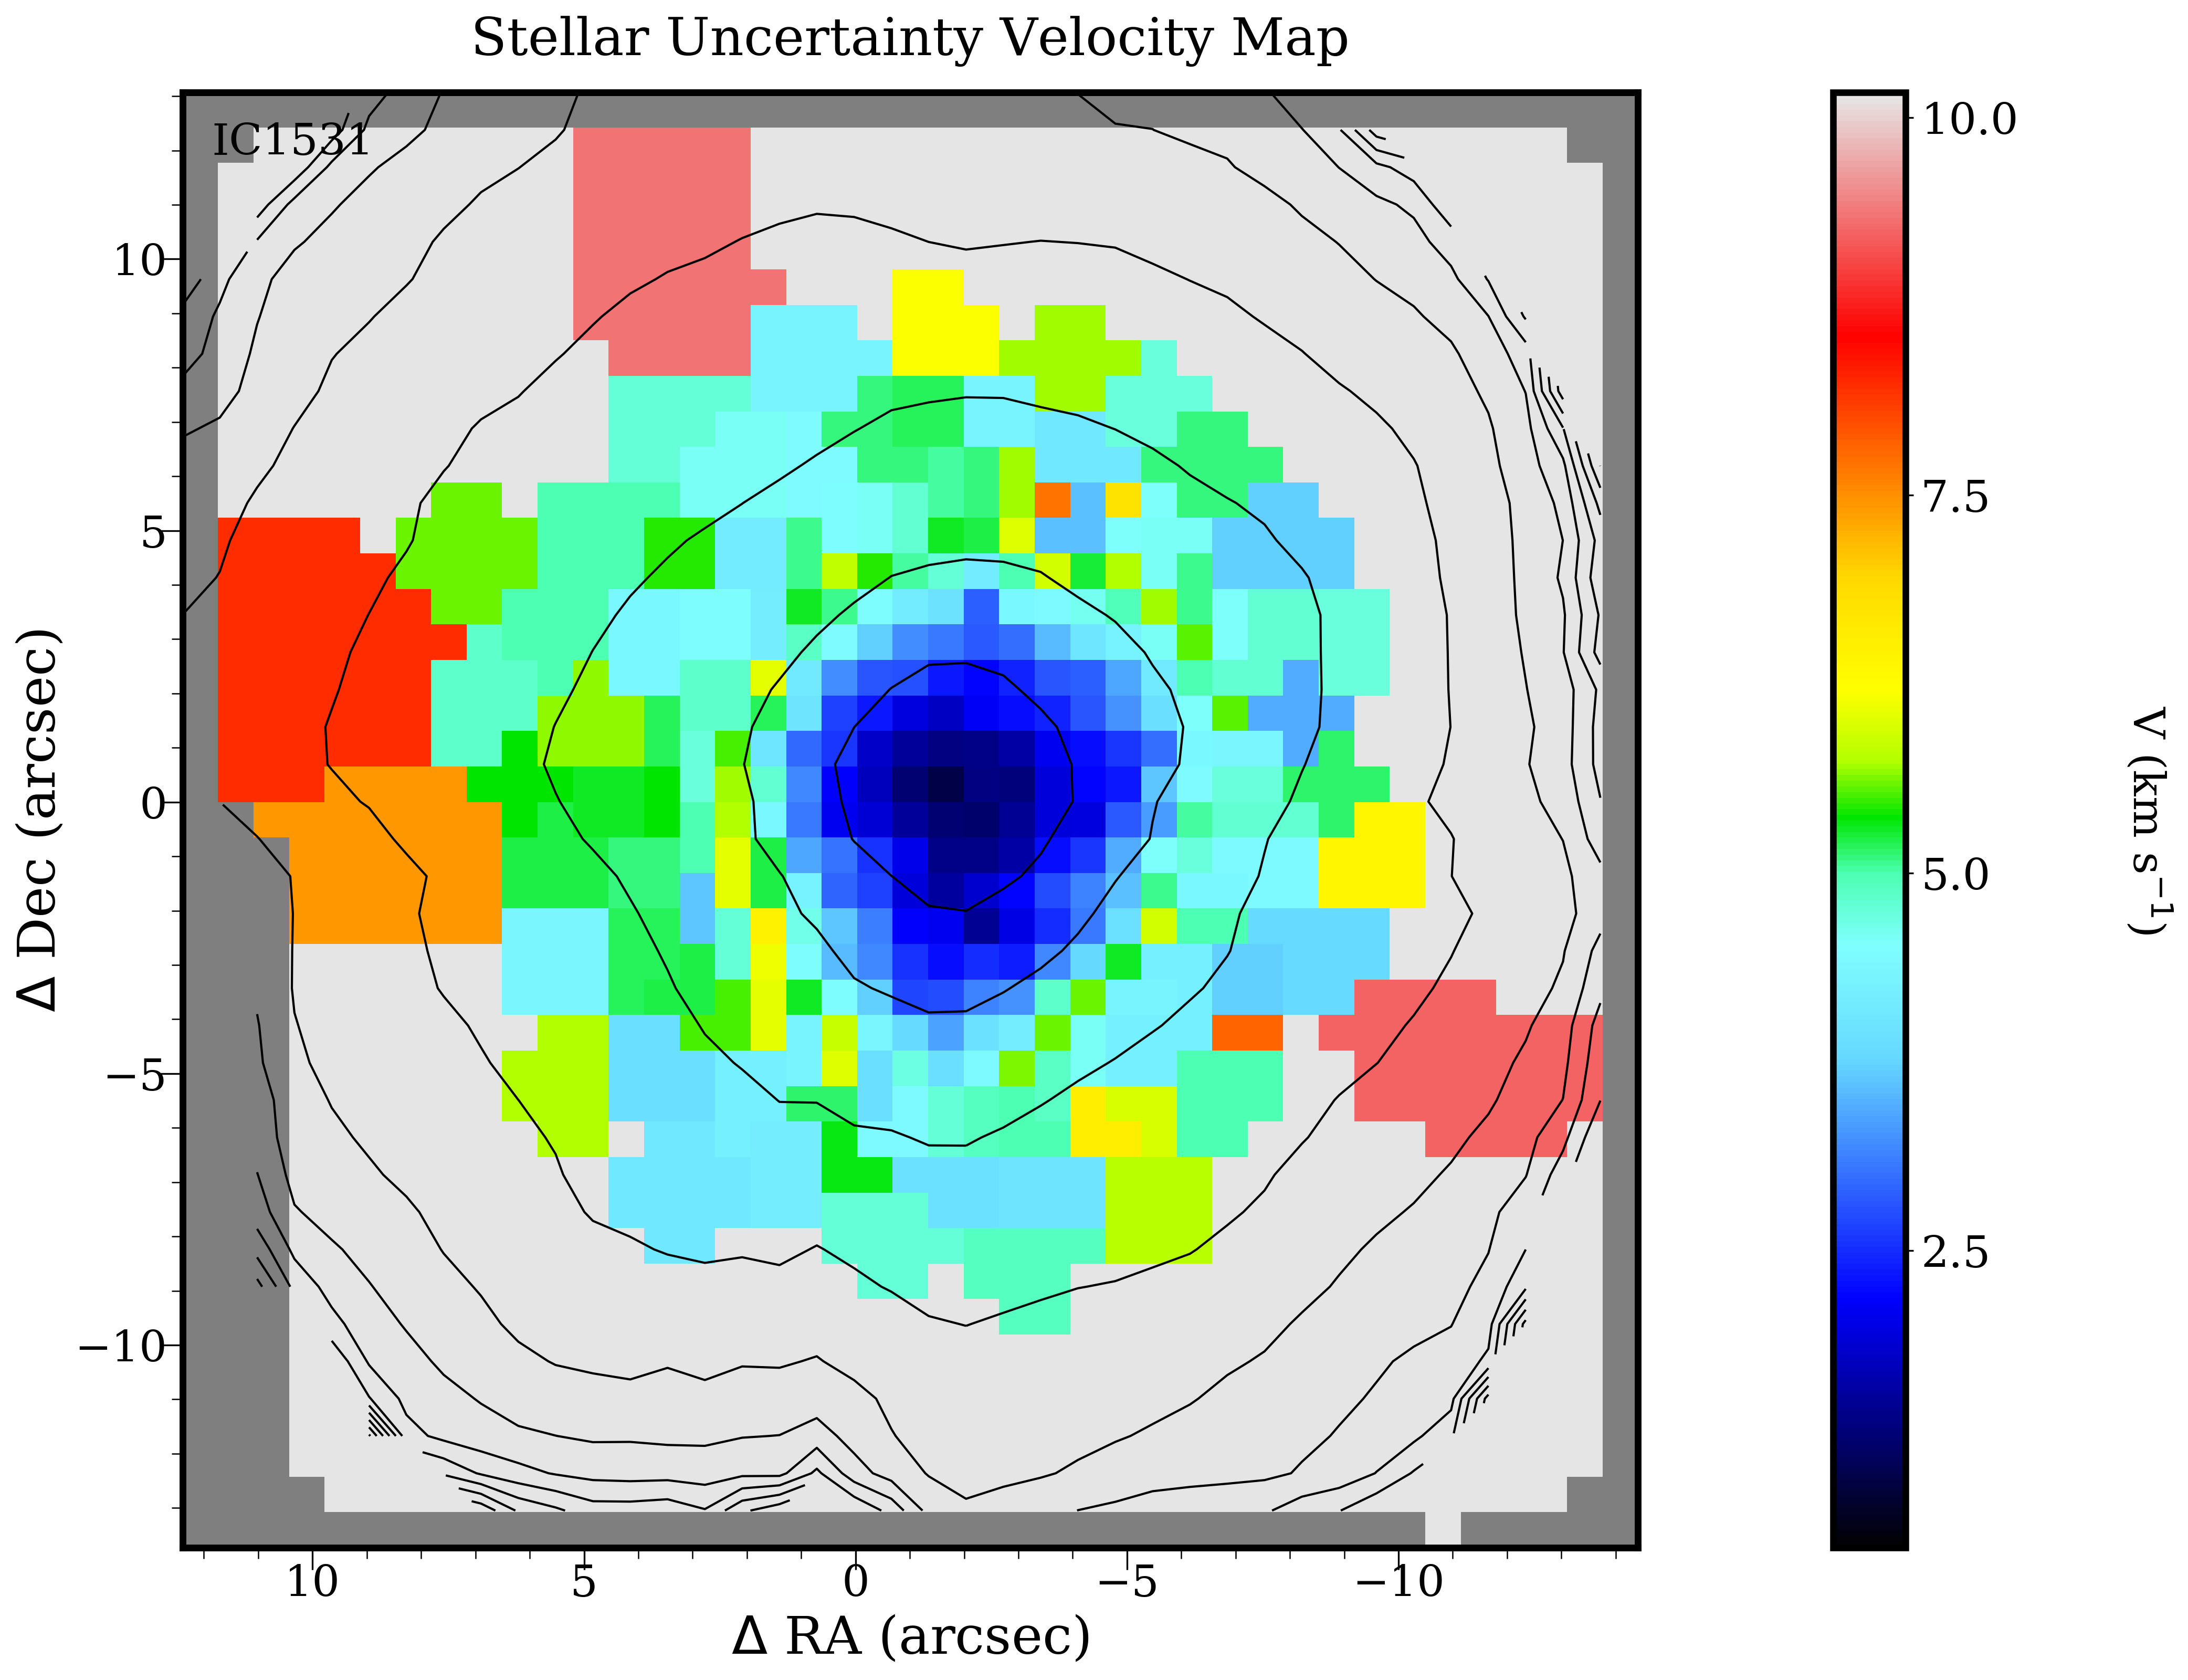
\includegraphics[width=0.245\textwidth]{Vmaps/ic1531_stellar_vel_uncert.png}
      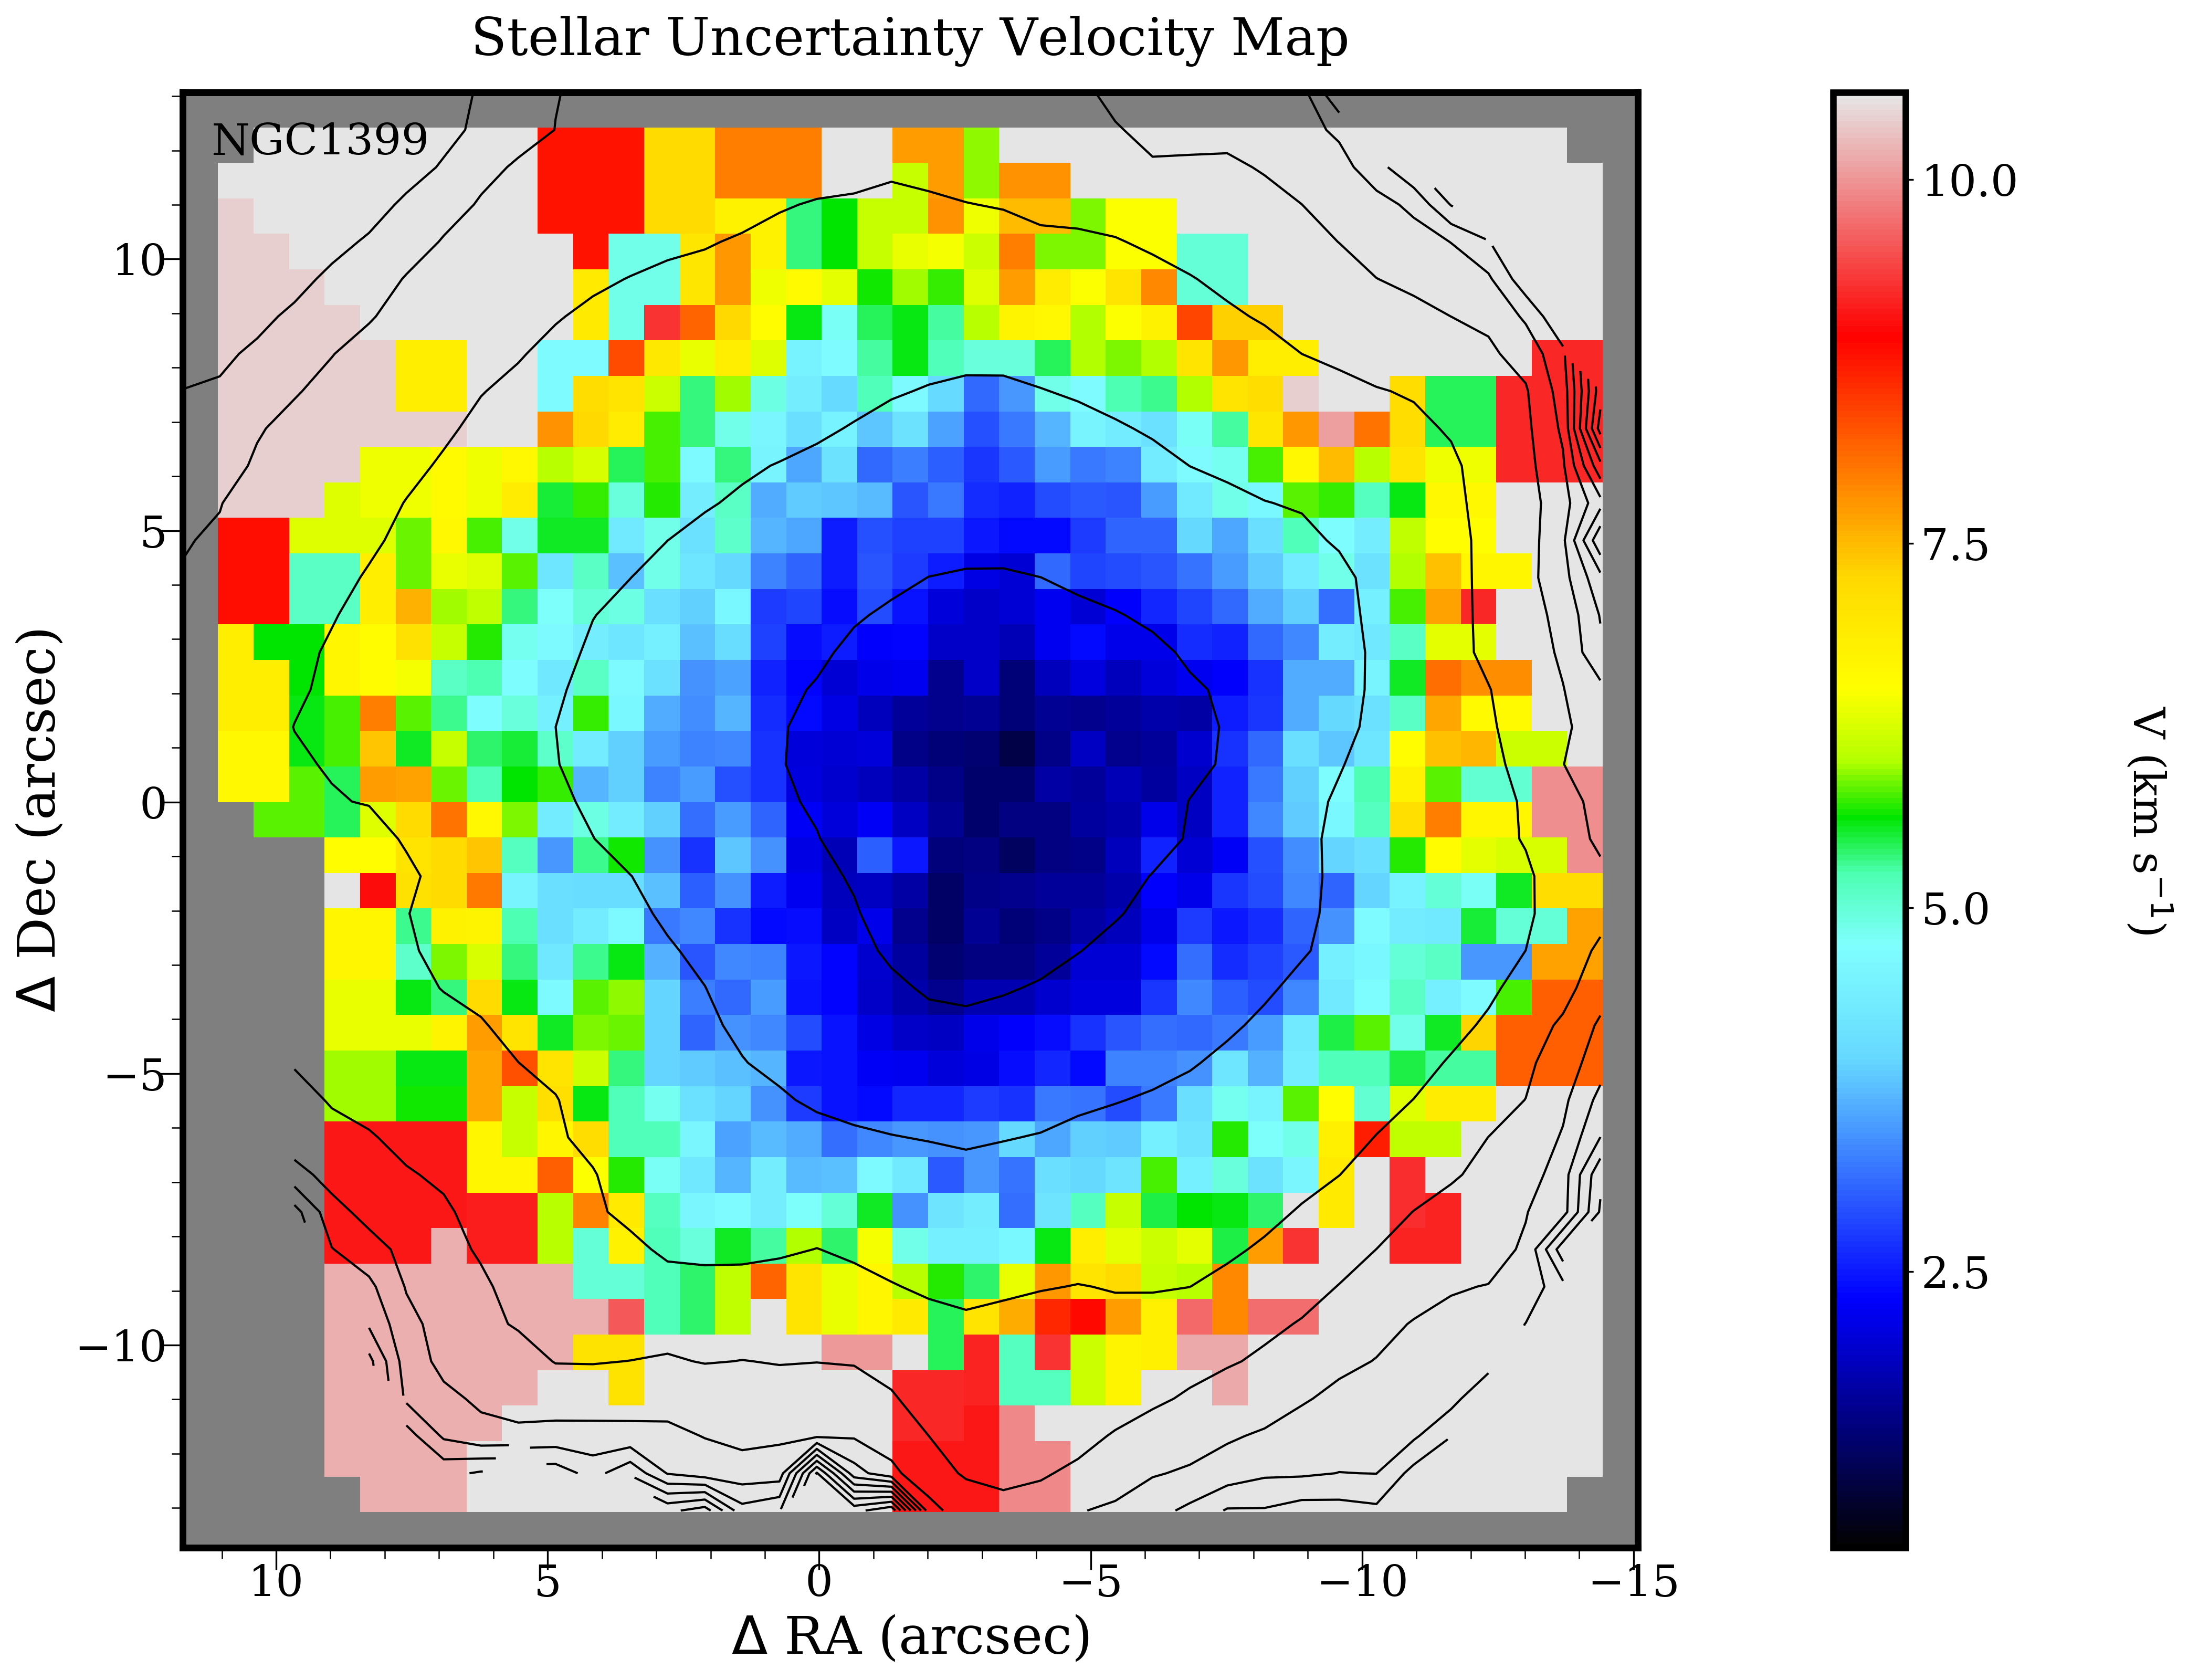
\includegraphics[width=0.245\textwidth]{Vmaps/ngc1399_stellar_vel_uncert.png}
      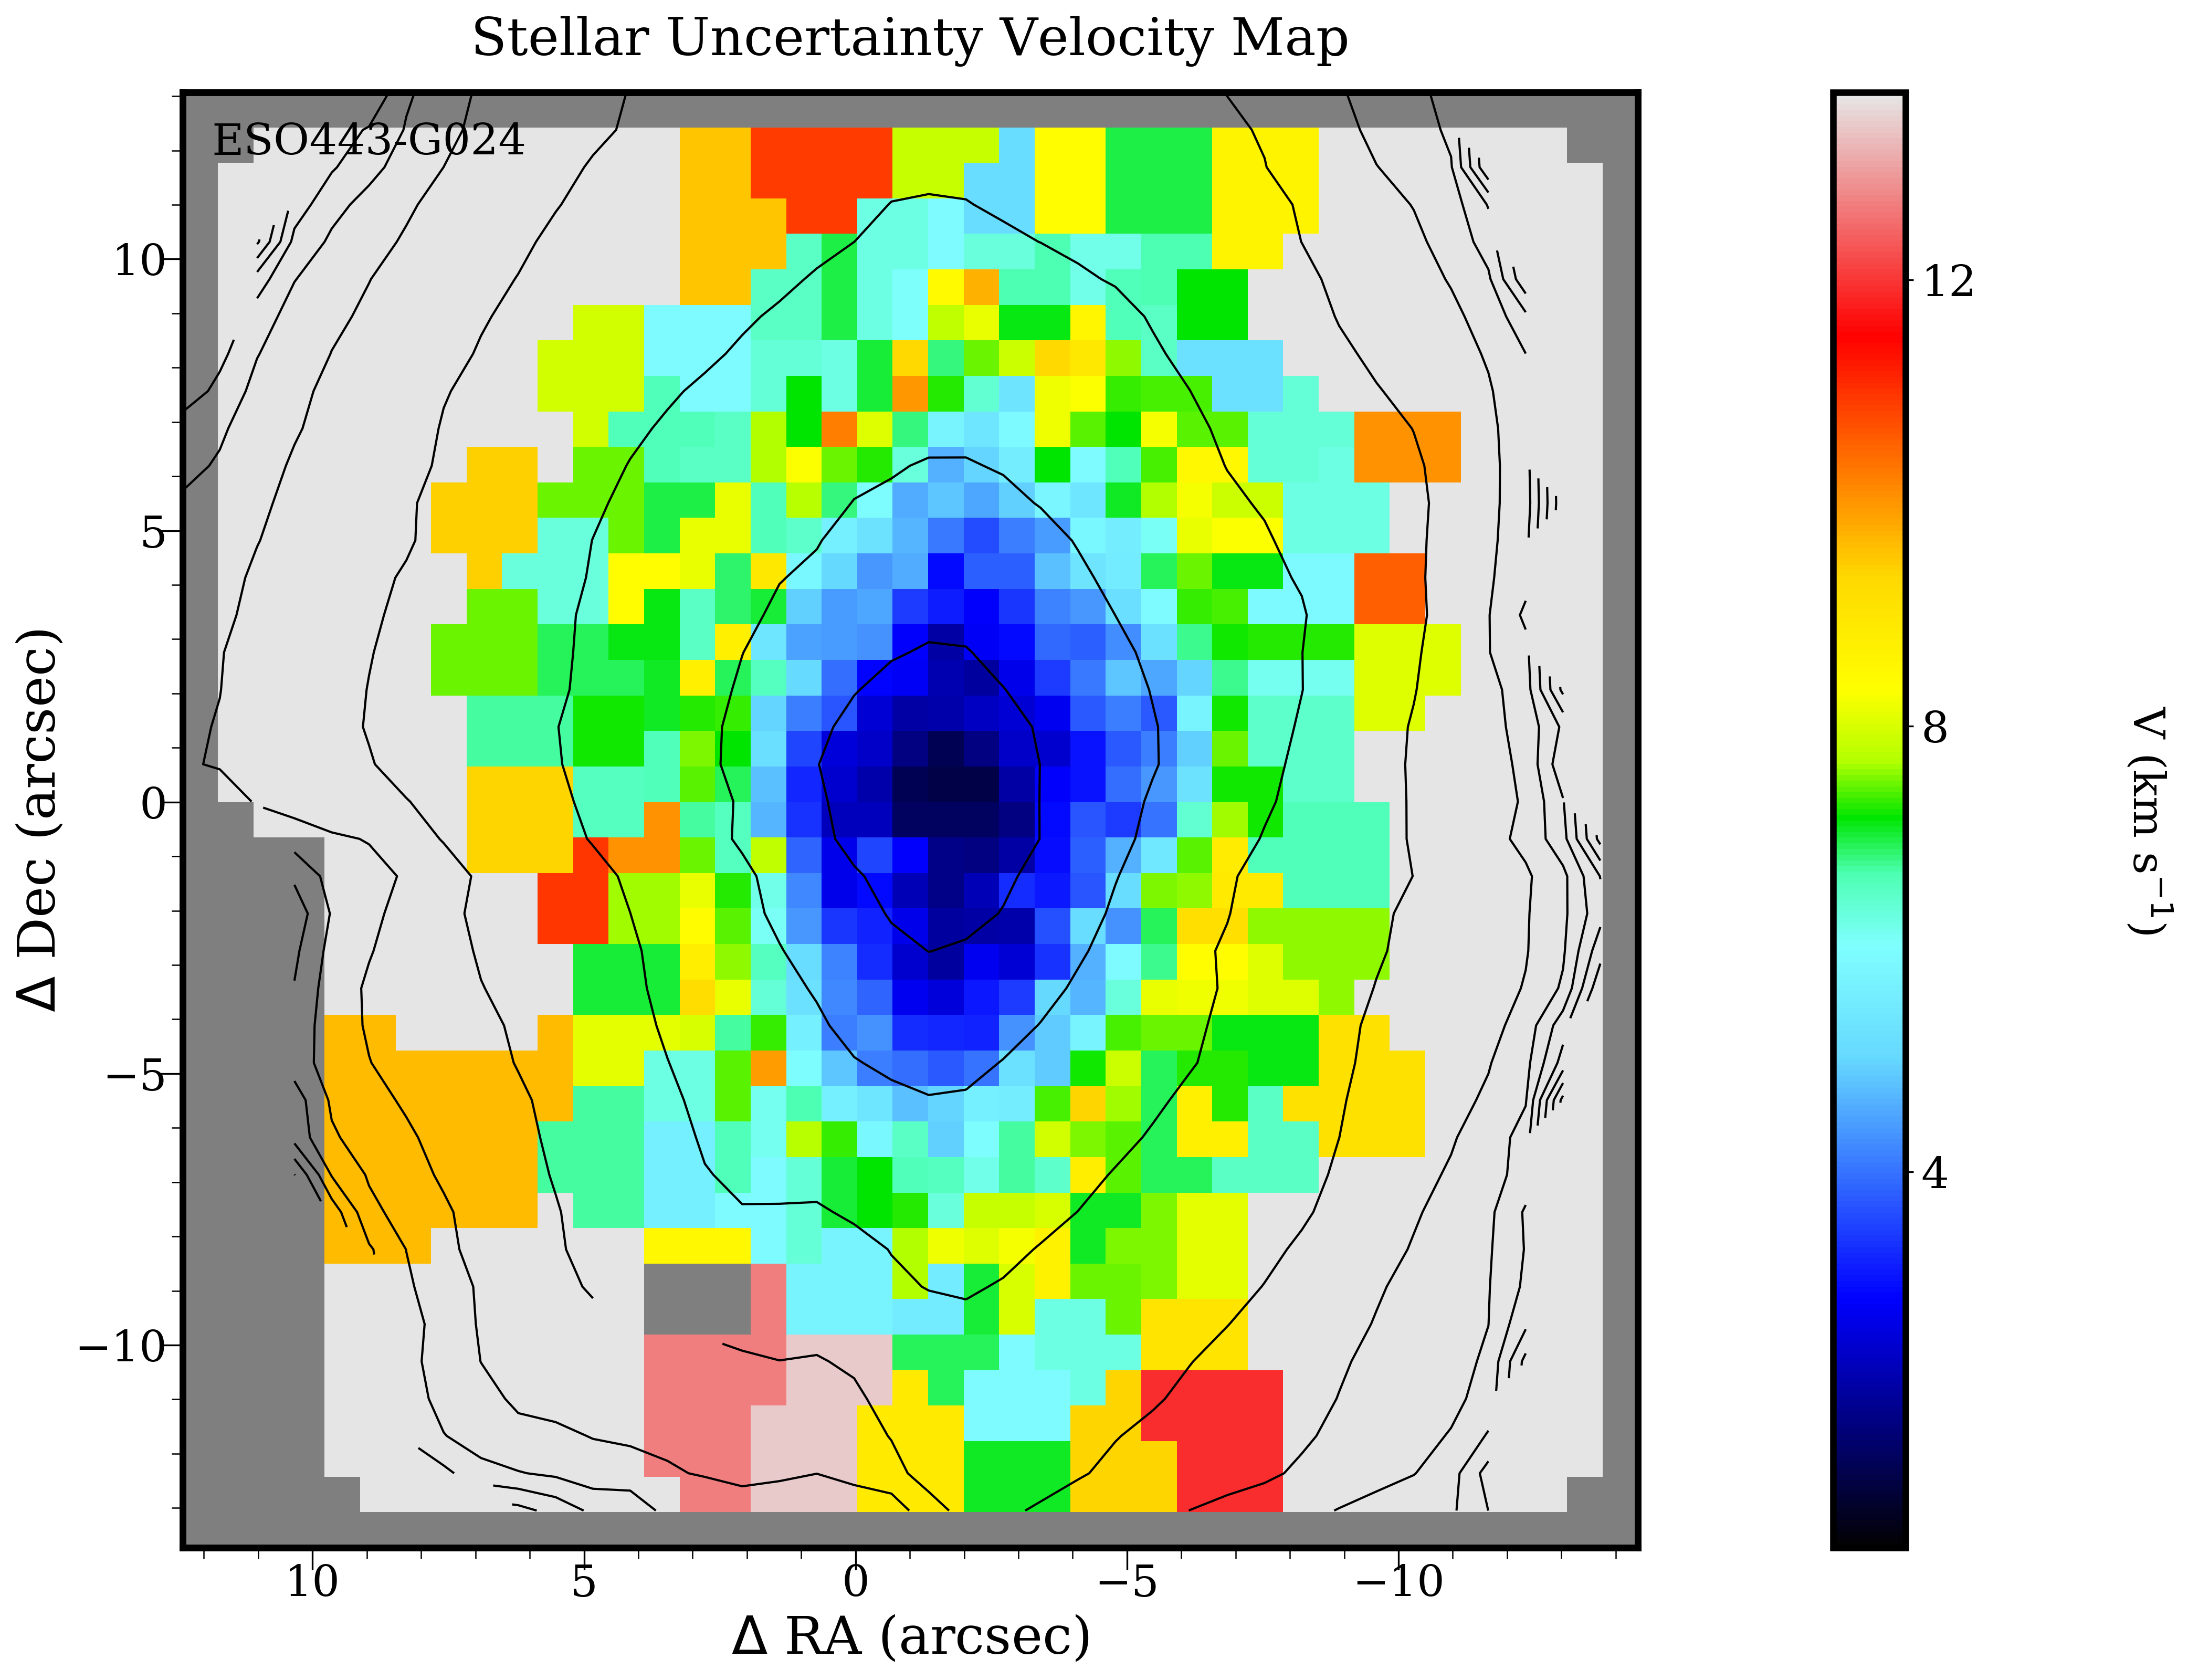
\includegraphics[width=0.245\textwidth]{Vmaps/eso443-g024_stellar_vel_uncert.png}
      \caption[VIMOS velocity uncertocity maps]{Uncertainties in the velocity for each galaxy in the VIMOS sample. Plots are ordered and contour colors are as in figure \ref{fig:Vstellar_img}}
      \label{fig:Vstellar_vel_uncert}
\end{figure*}

\begin{figure*}
      \centering
      \includegraphics[width=0.245\textwidth]{Vmaps/ngc0612_stellar_sigma.png}
      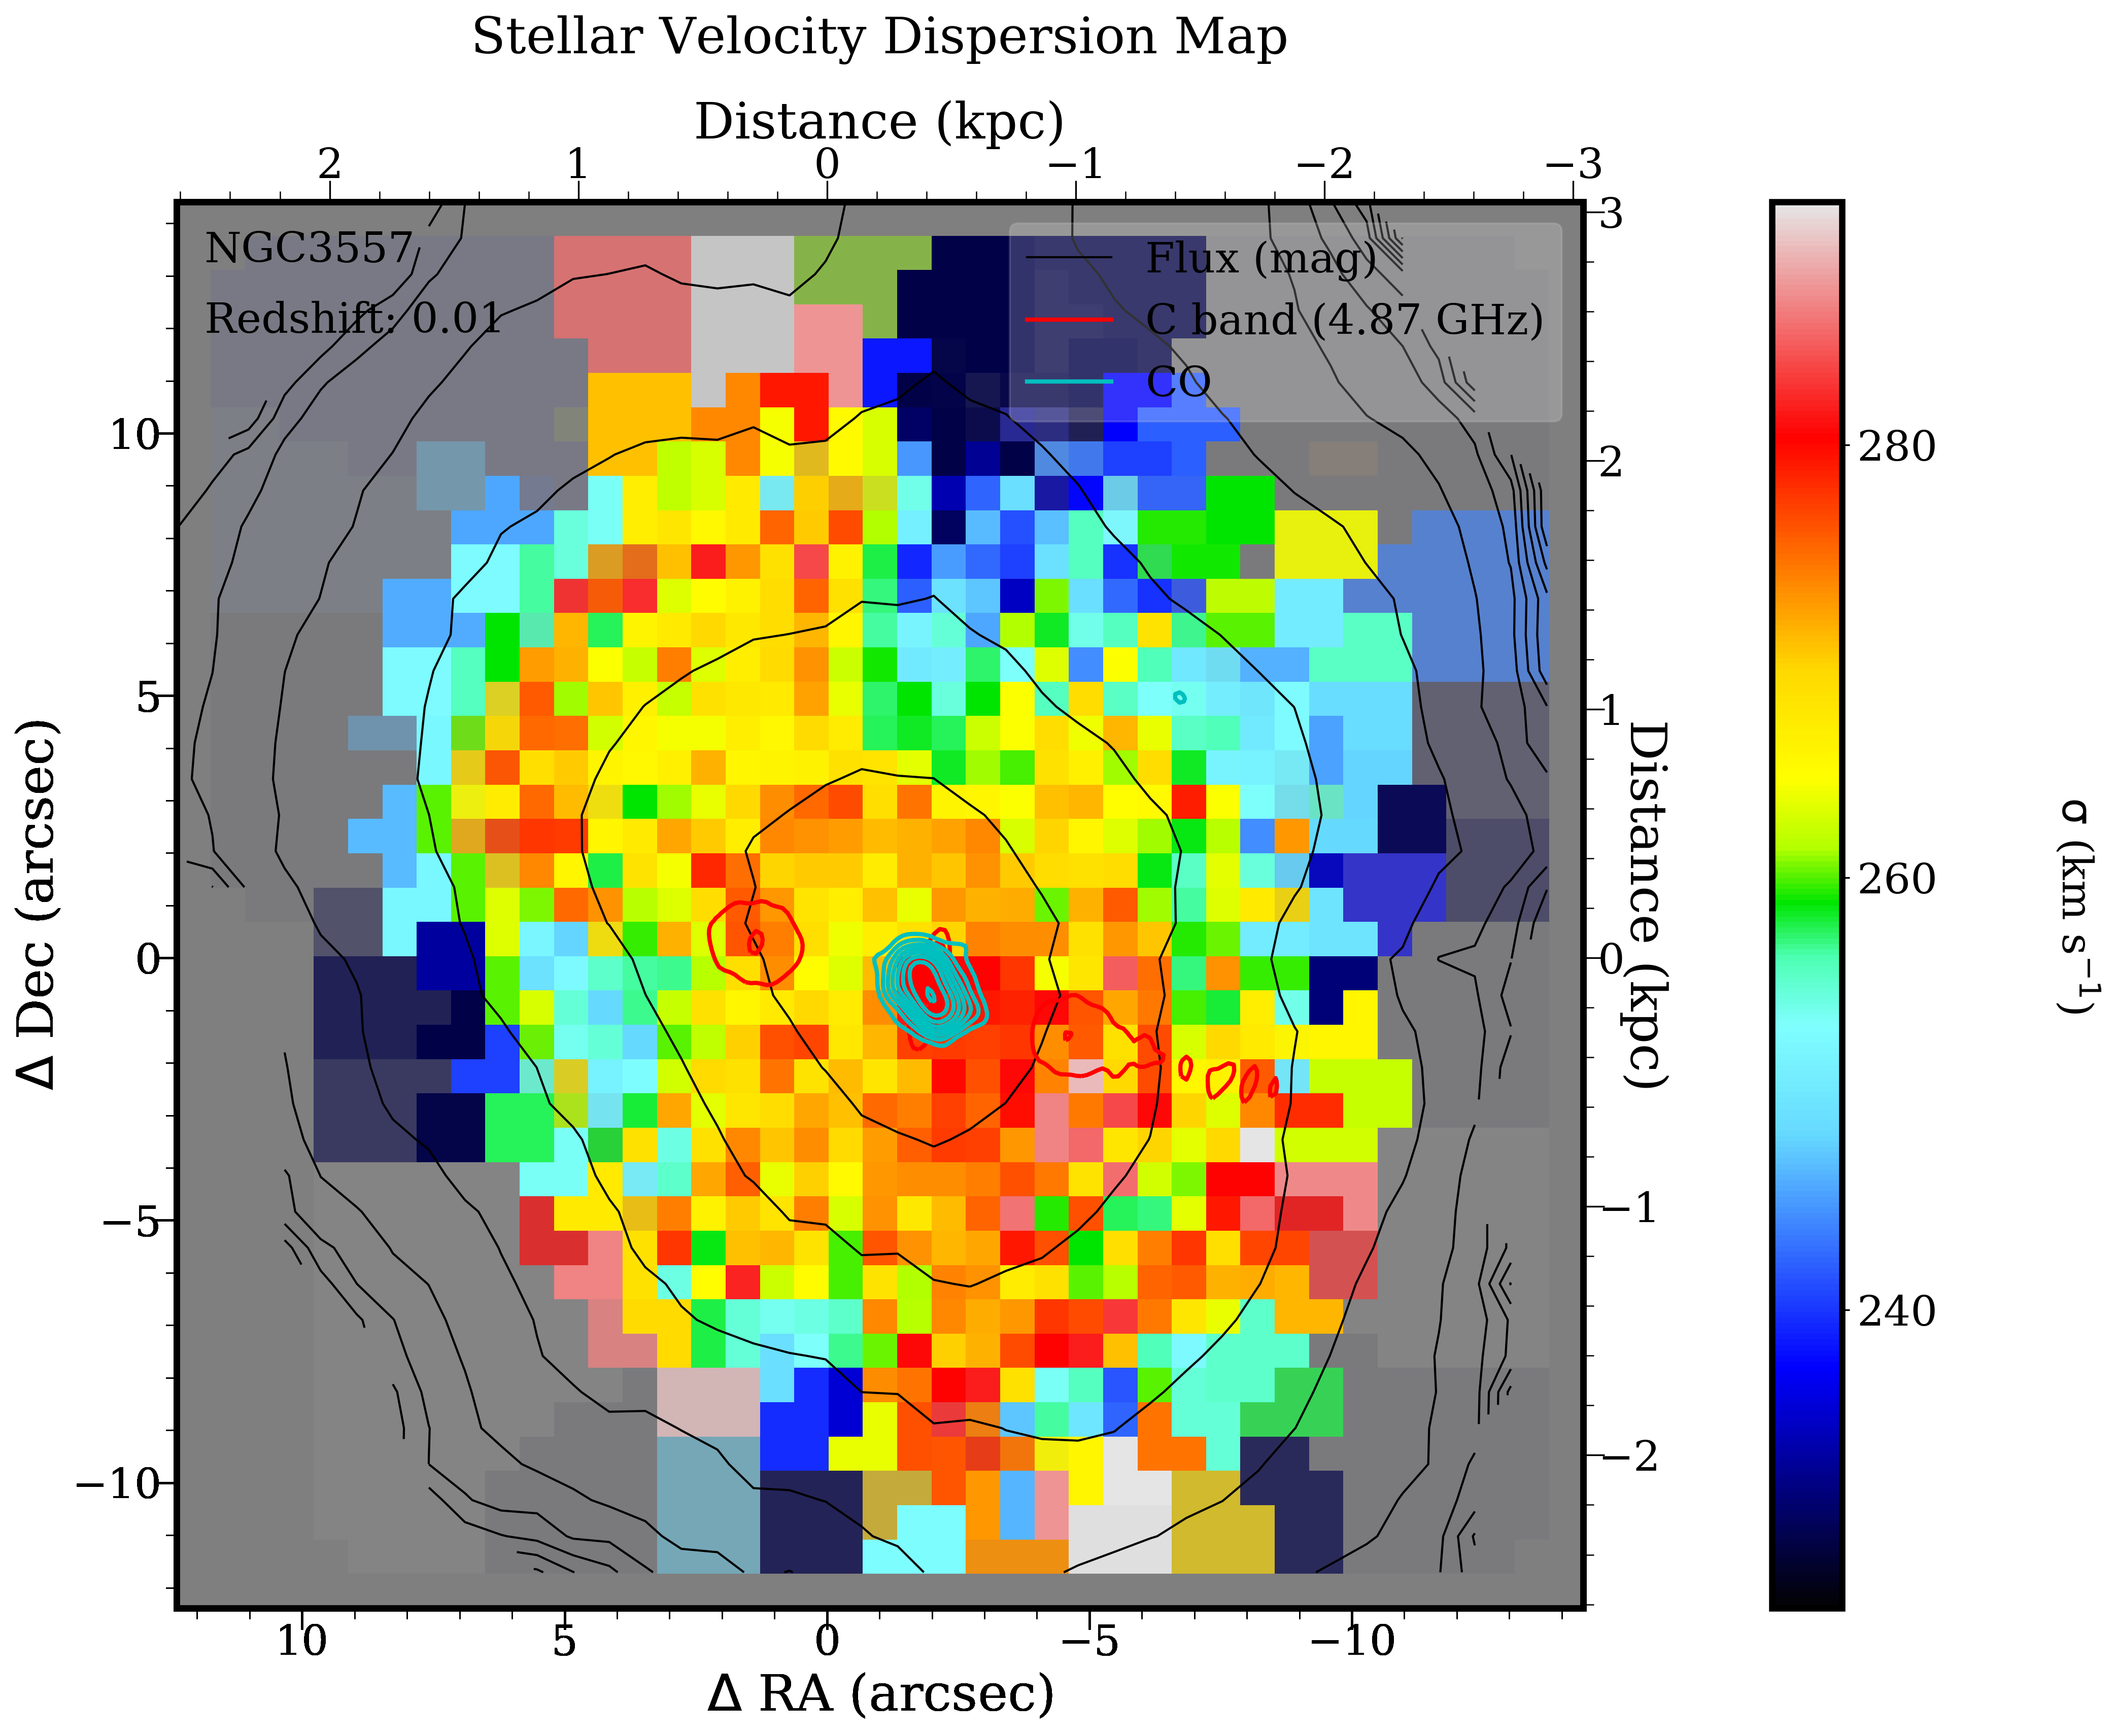
\includegraphics[width=0.245\textwidth]{Vmaps/ngc3557_stellar_sigma.png}
      \includegraphics[width=0.245\textwidth]{Vmaps/ngc3100_stellar_sigma.png}
      \includegraphics[width=0.245\textwidth]{Vmaps/ic1459_stellar_sigma.png}
      \includegraphics[width=0.245\textwidth]{Vmaps/pks0718-34_stellar_sigma.png}
      \includegraphics[width=0.245\textwidth]{Vmaps/ic4296_stellar_sigma.png}
      \includegraphics[width=0.245\textwidth]{Vmaps/ngc7075_stellar_sigma.png}
      \includegraphics[width=0.245\textwidth]{Vmaps/ic1531_stellar_sigma.png}
      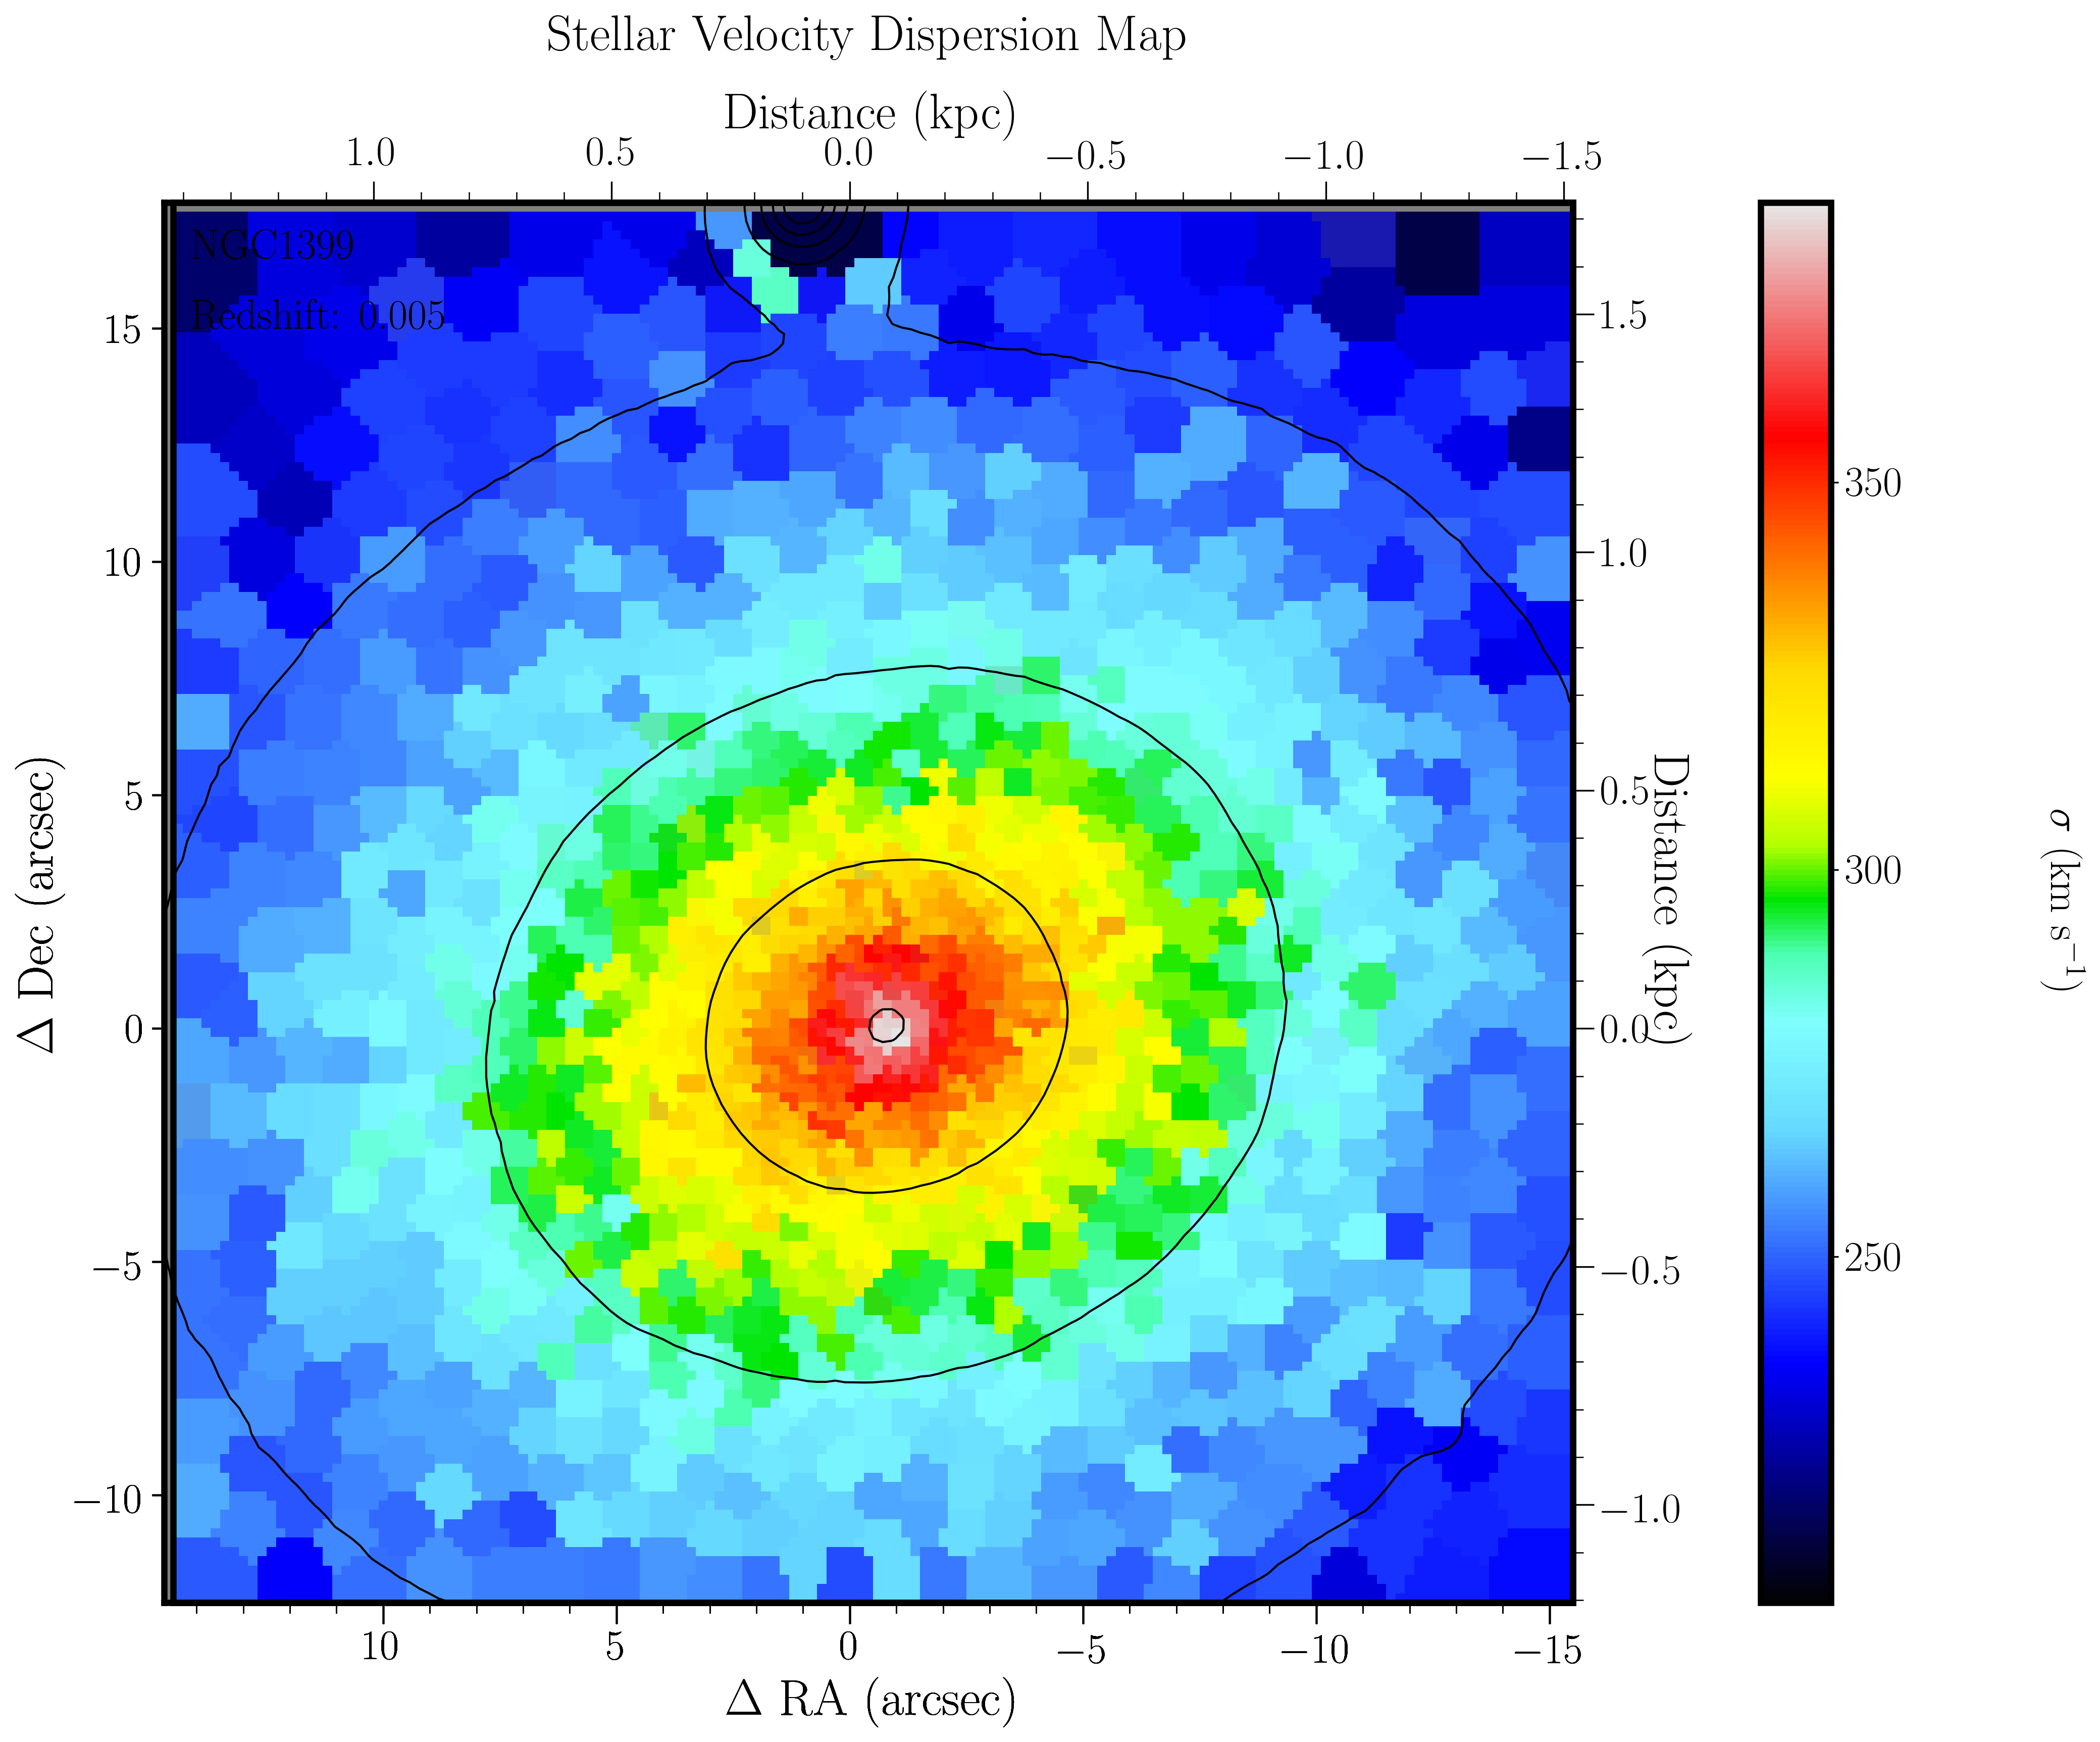
\includegraphics[width=0.245\textwidth]{Vmaps/ngc1399_stellar_sigma.png}
      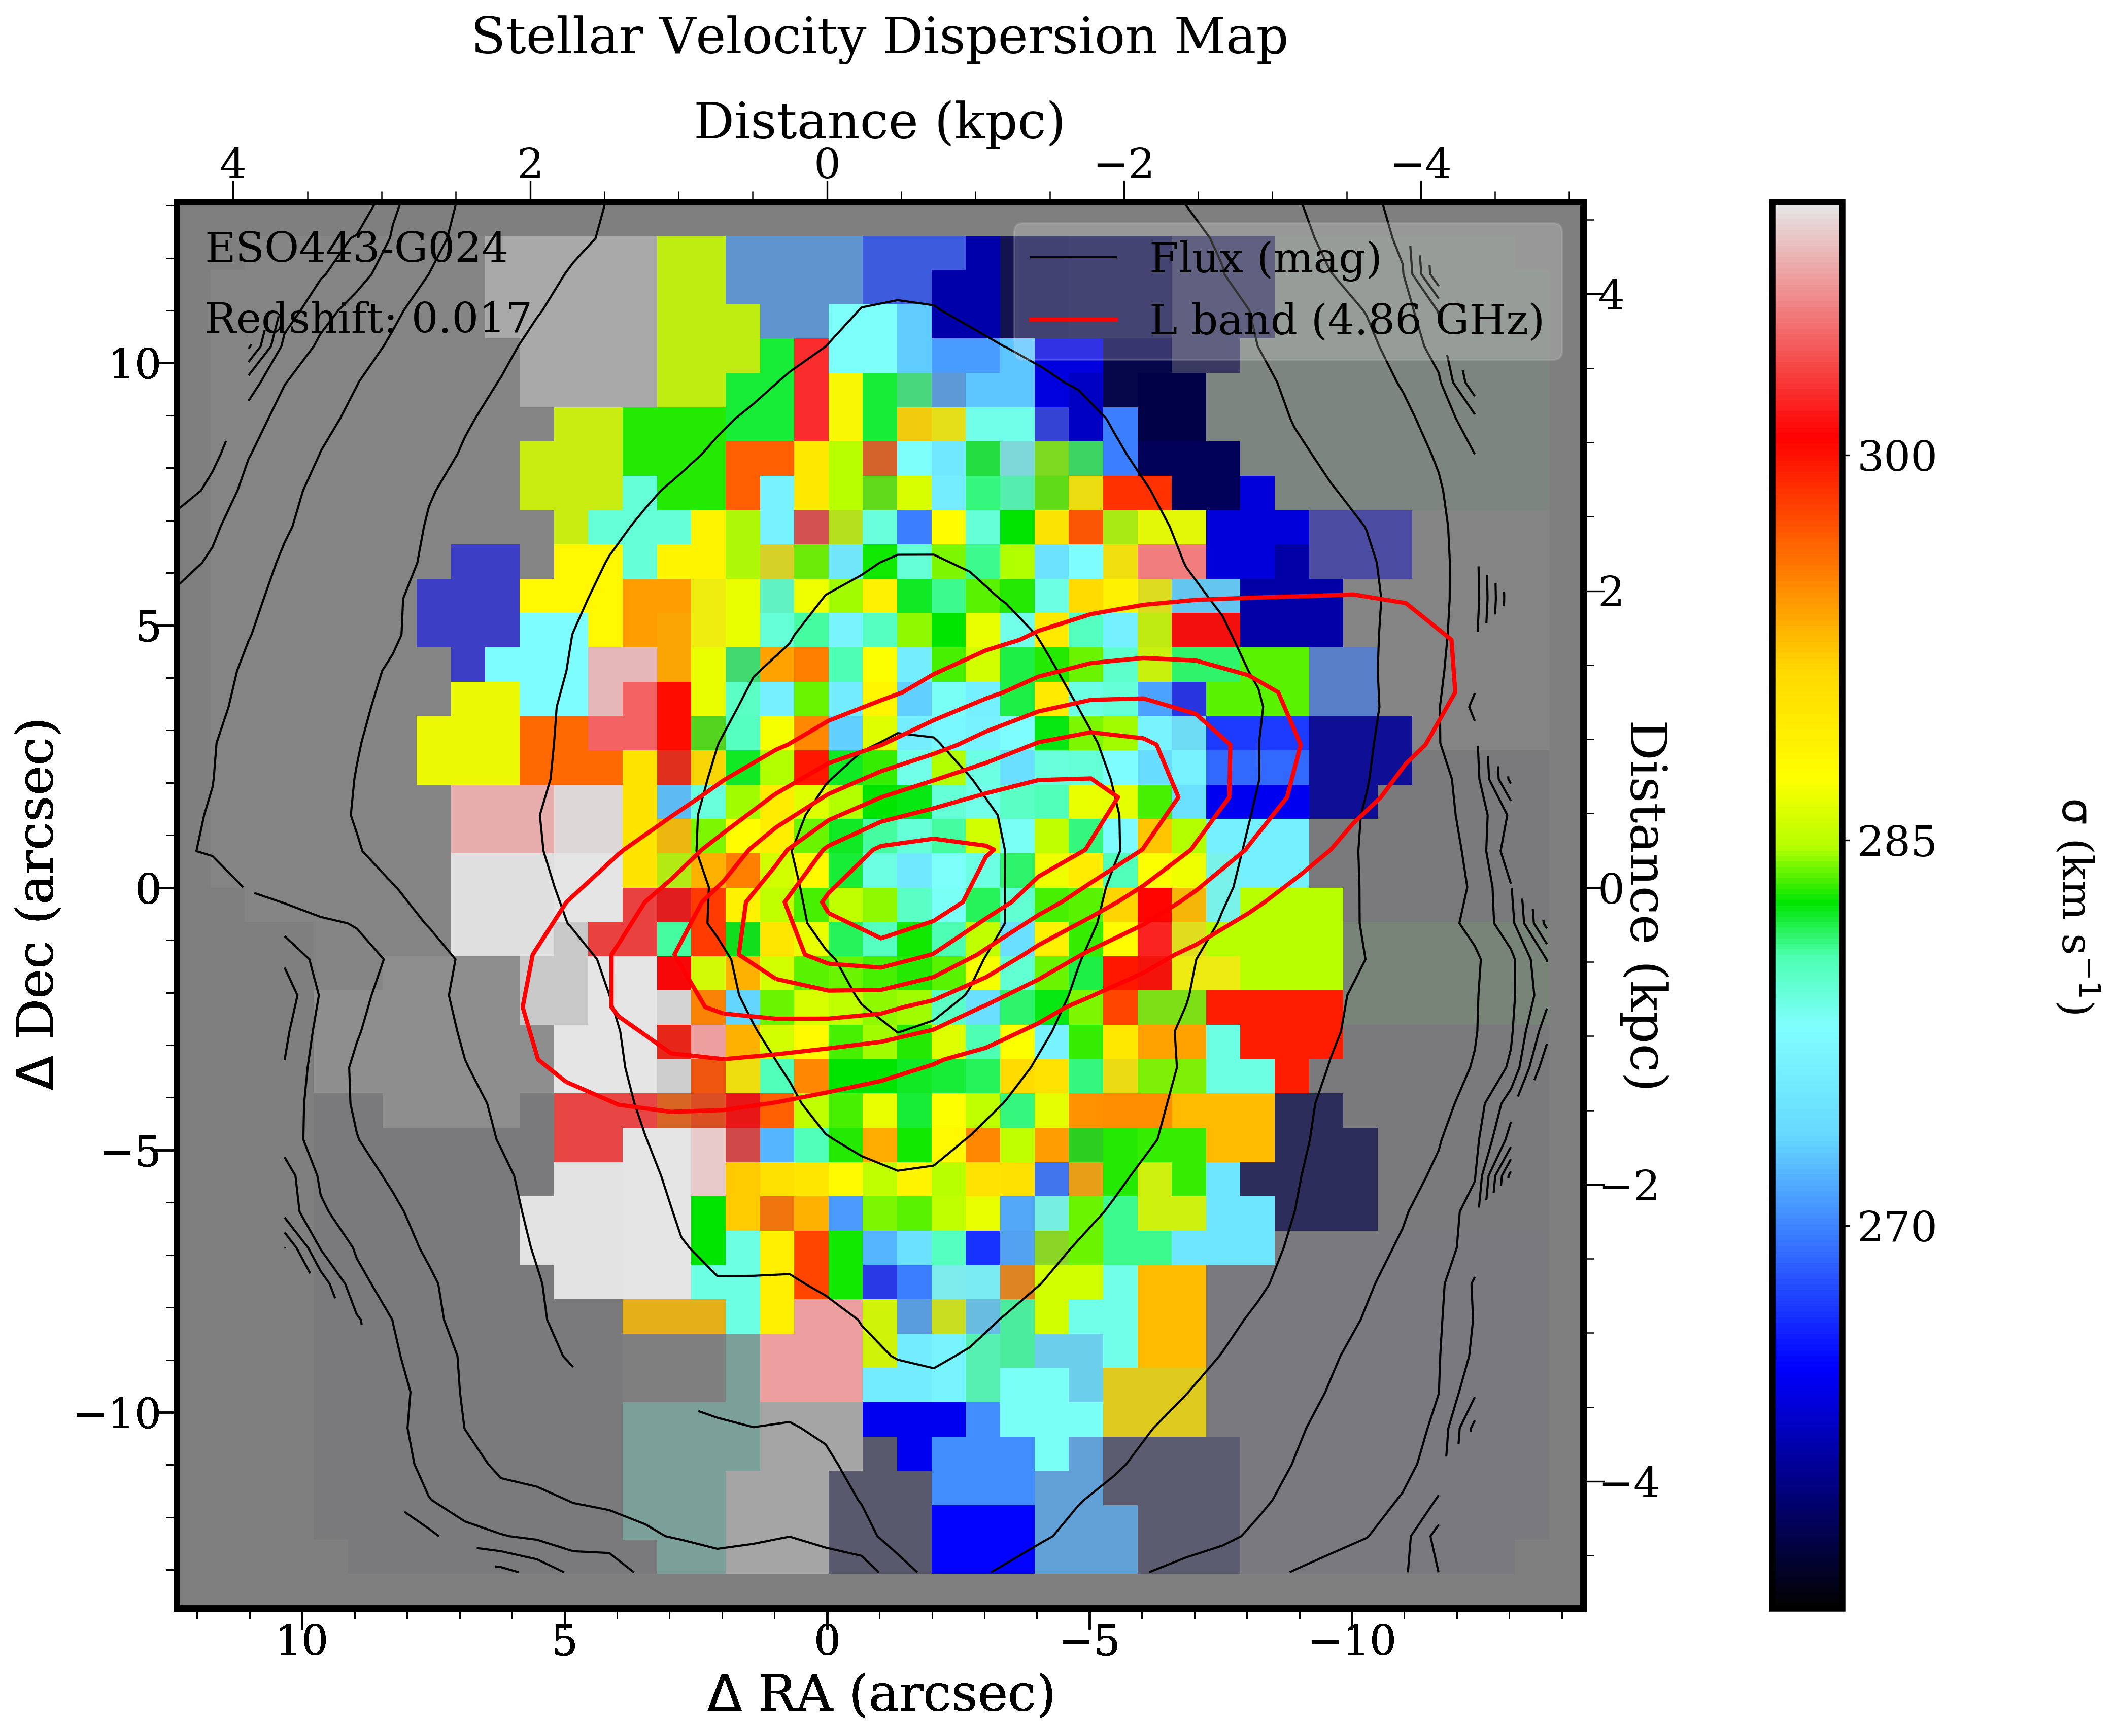
\includegraphics[width=0.245\textwidth]{Vmaps/eso443-g024_stellar_sigma.png}
      \caption[VIMOS velocity dispersion]{Velocity dispersion for each galaxy in the VIMOS sample. Plots are ordered and contour colors are as in figure \ref{fig:Vstellar_img}}
      \label{fig:Vstellar_sigma}
\end{figure*}


\begin{figure*}
      \centering
      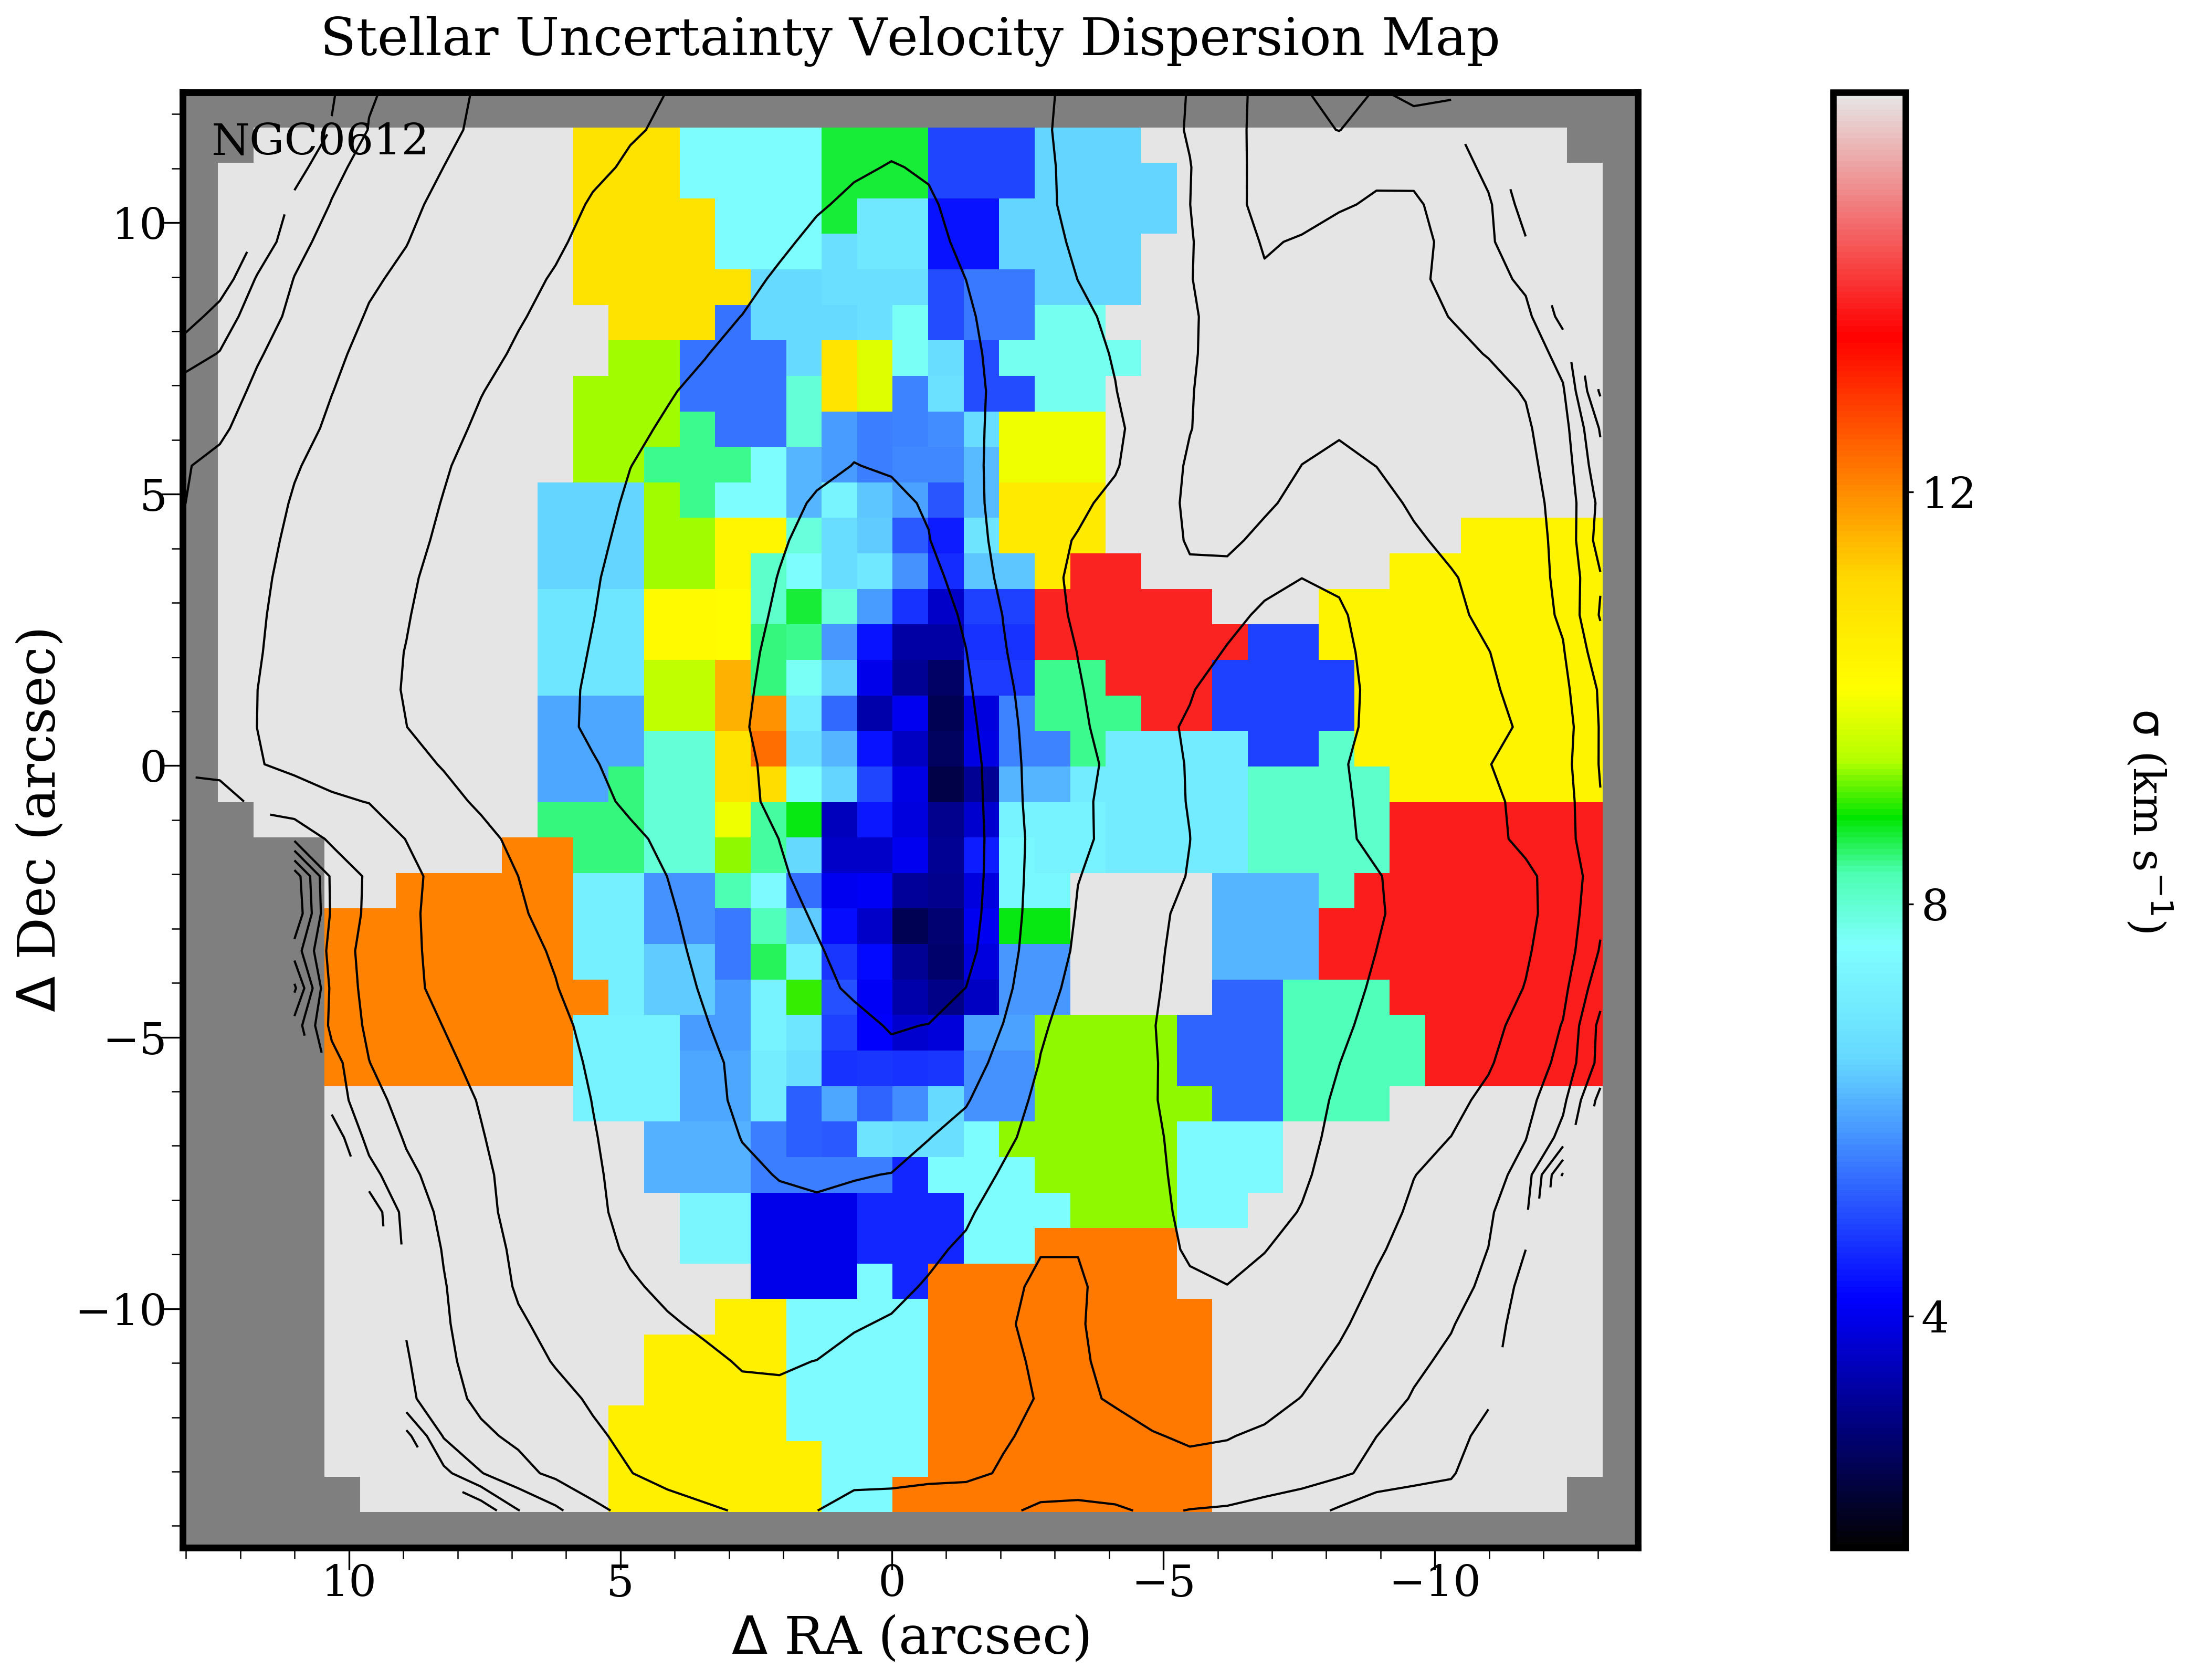
\includegraphics[width=0.245\textwidth]{Vmaps/ngc0612_stellar_sigma_uncert.png}
      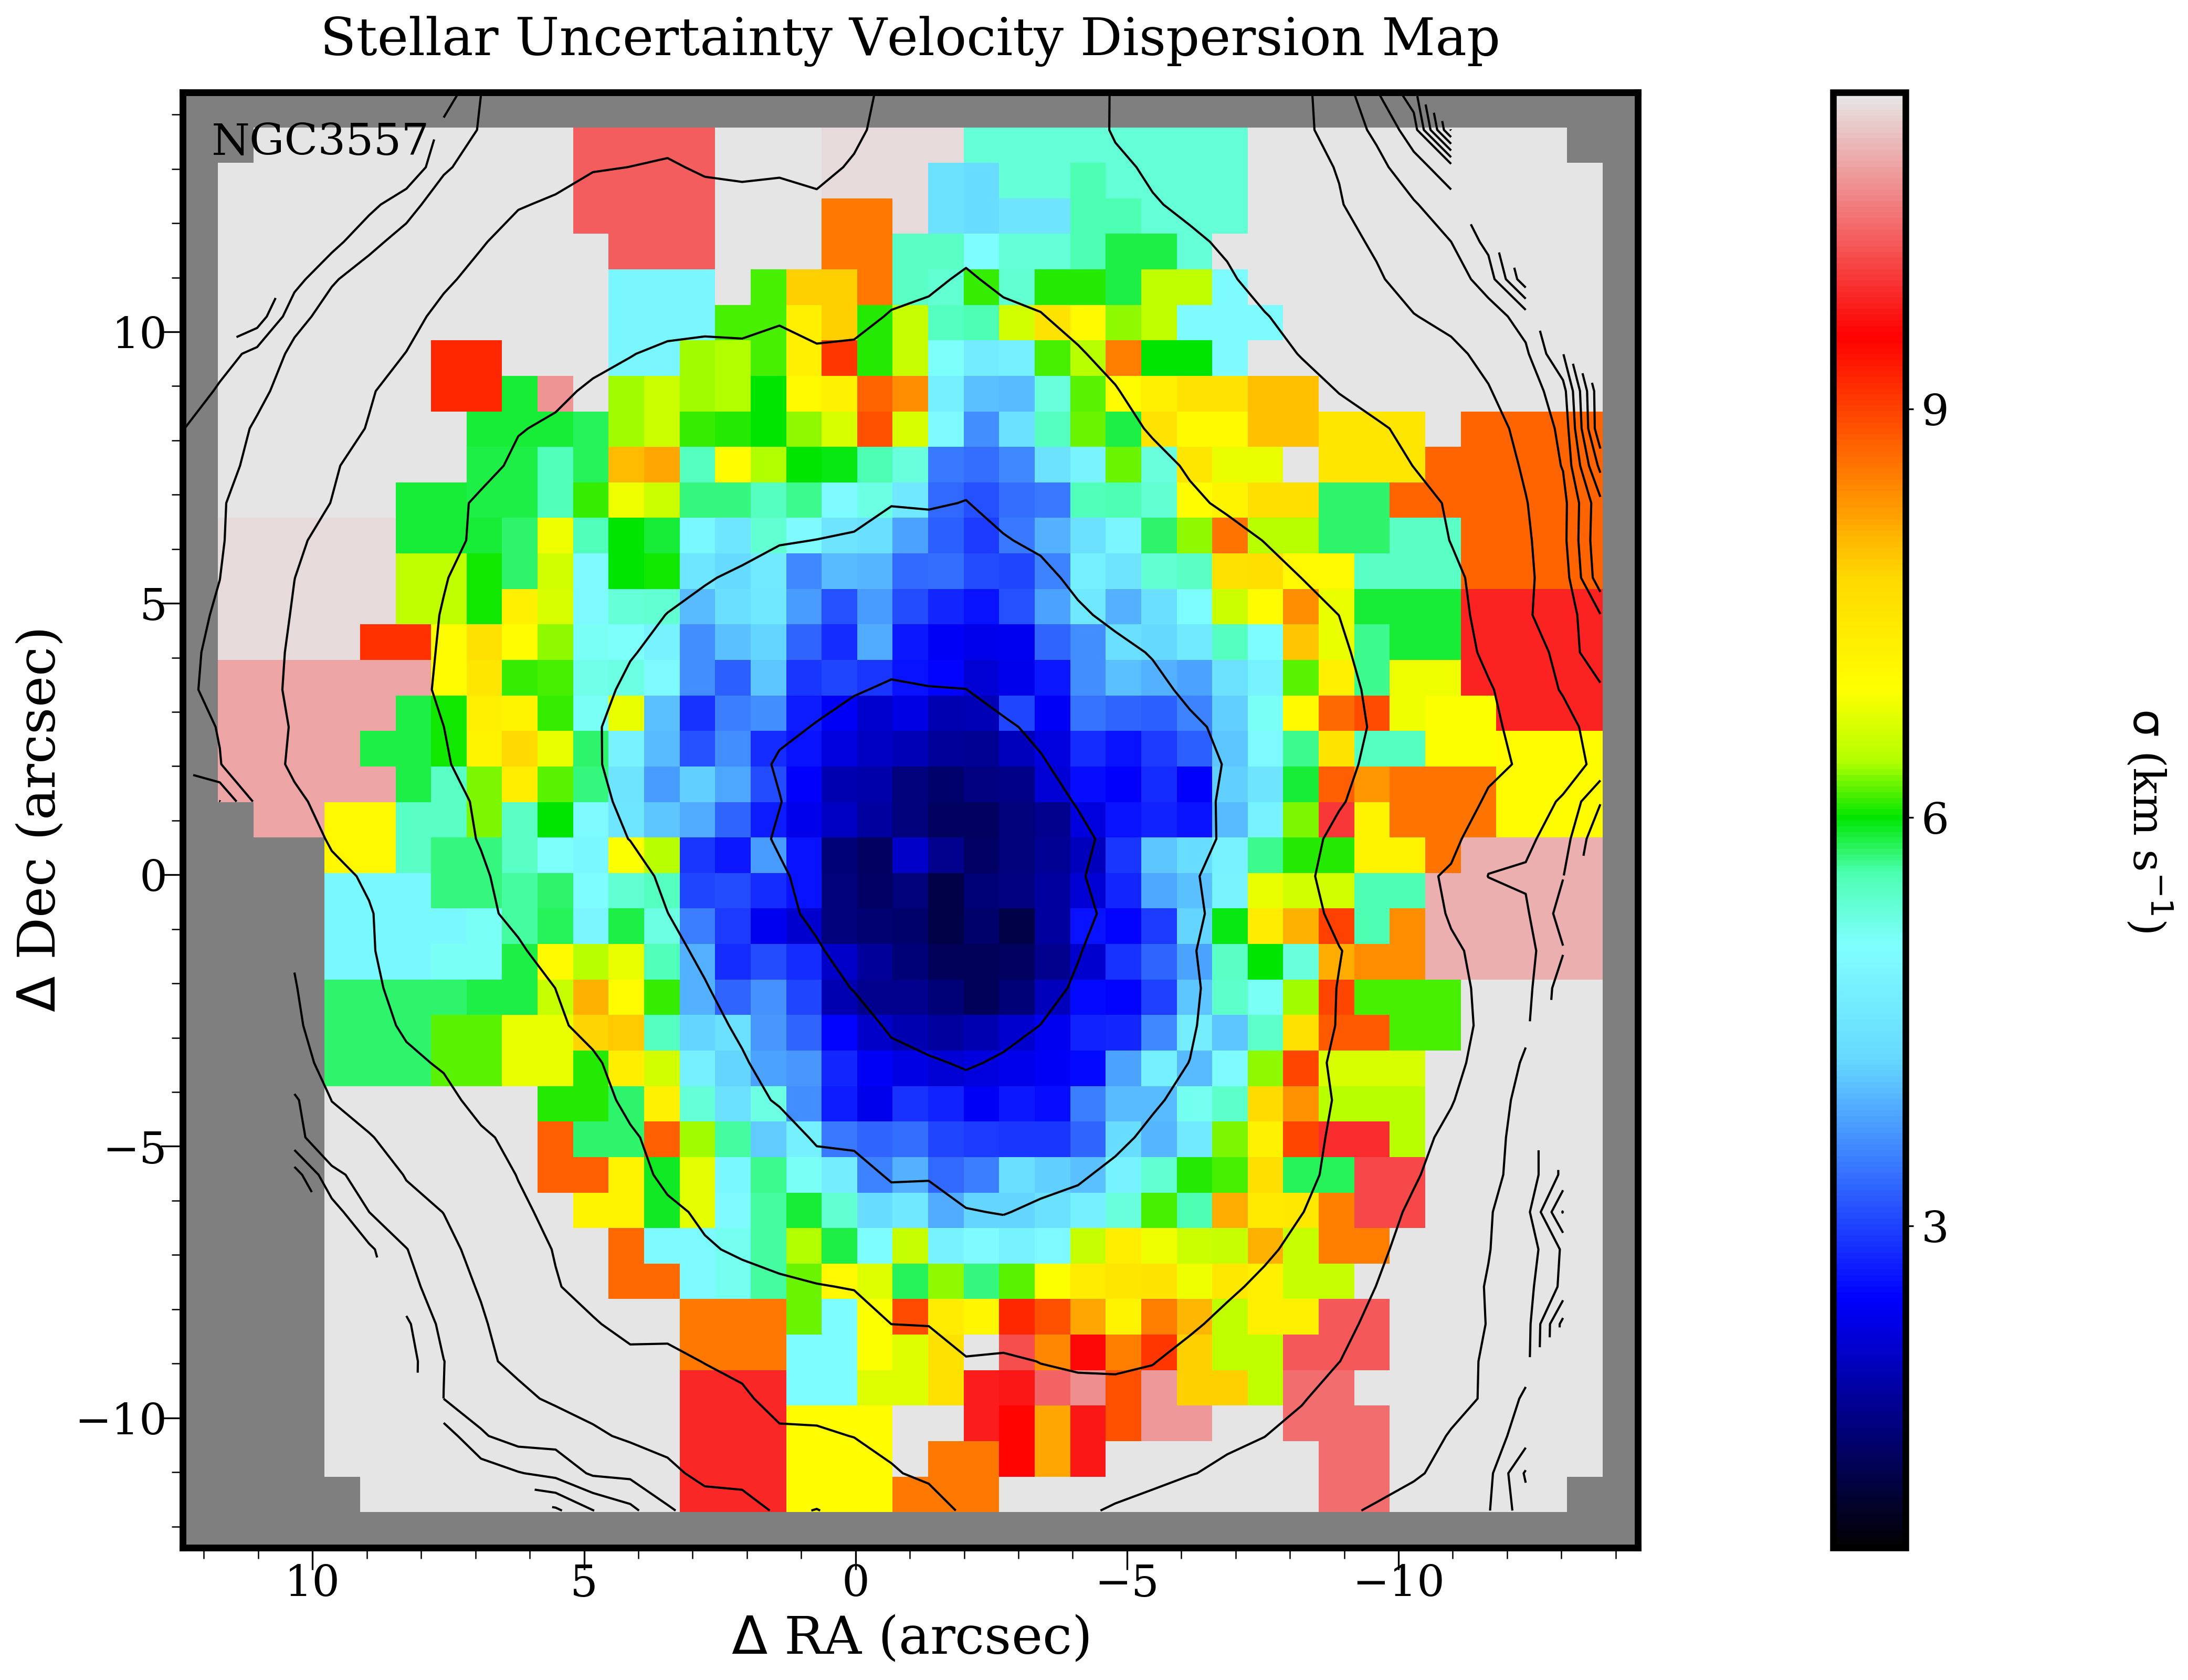
\includegraphics[width=0.245\textwidth]{Vmaps/ngc3557_stellar_sigma_uncert.png}
      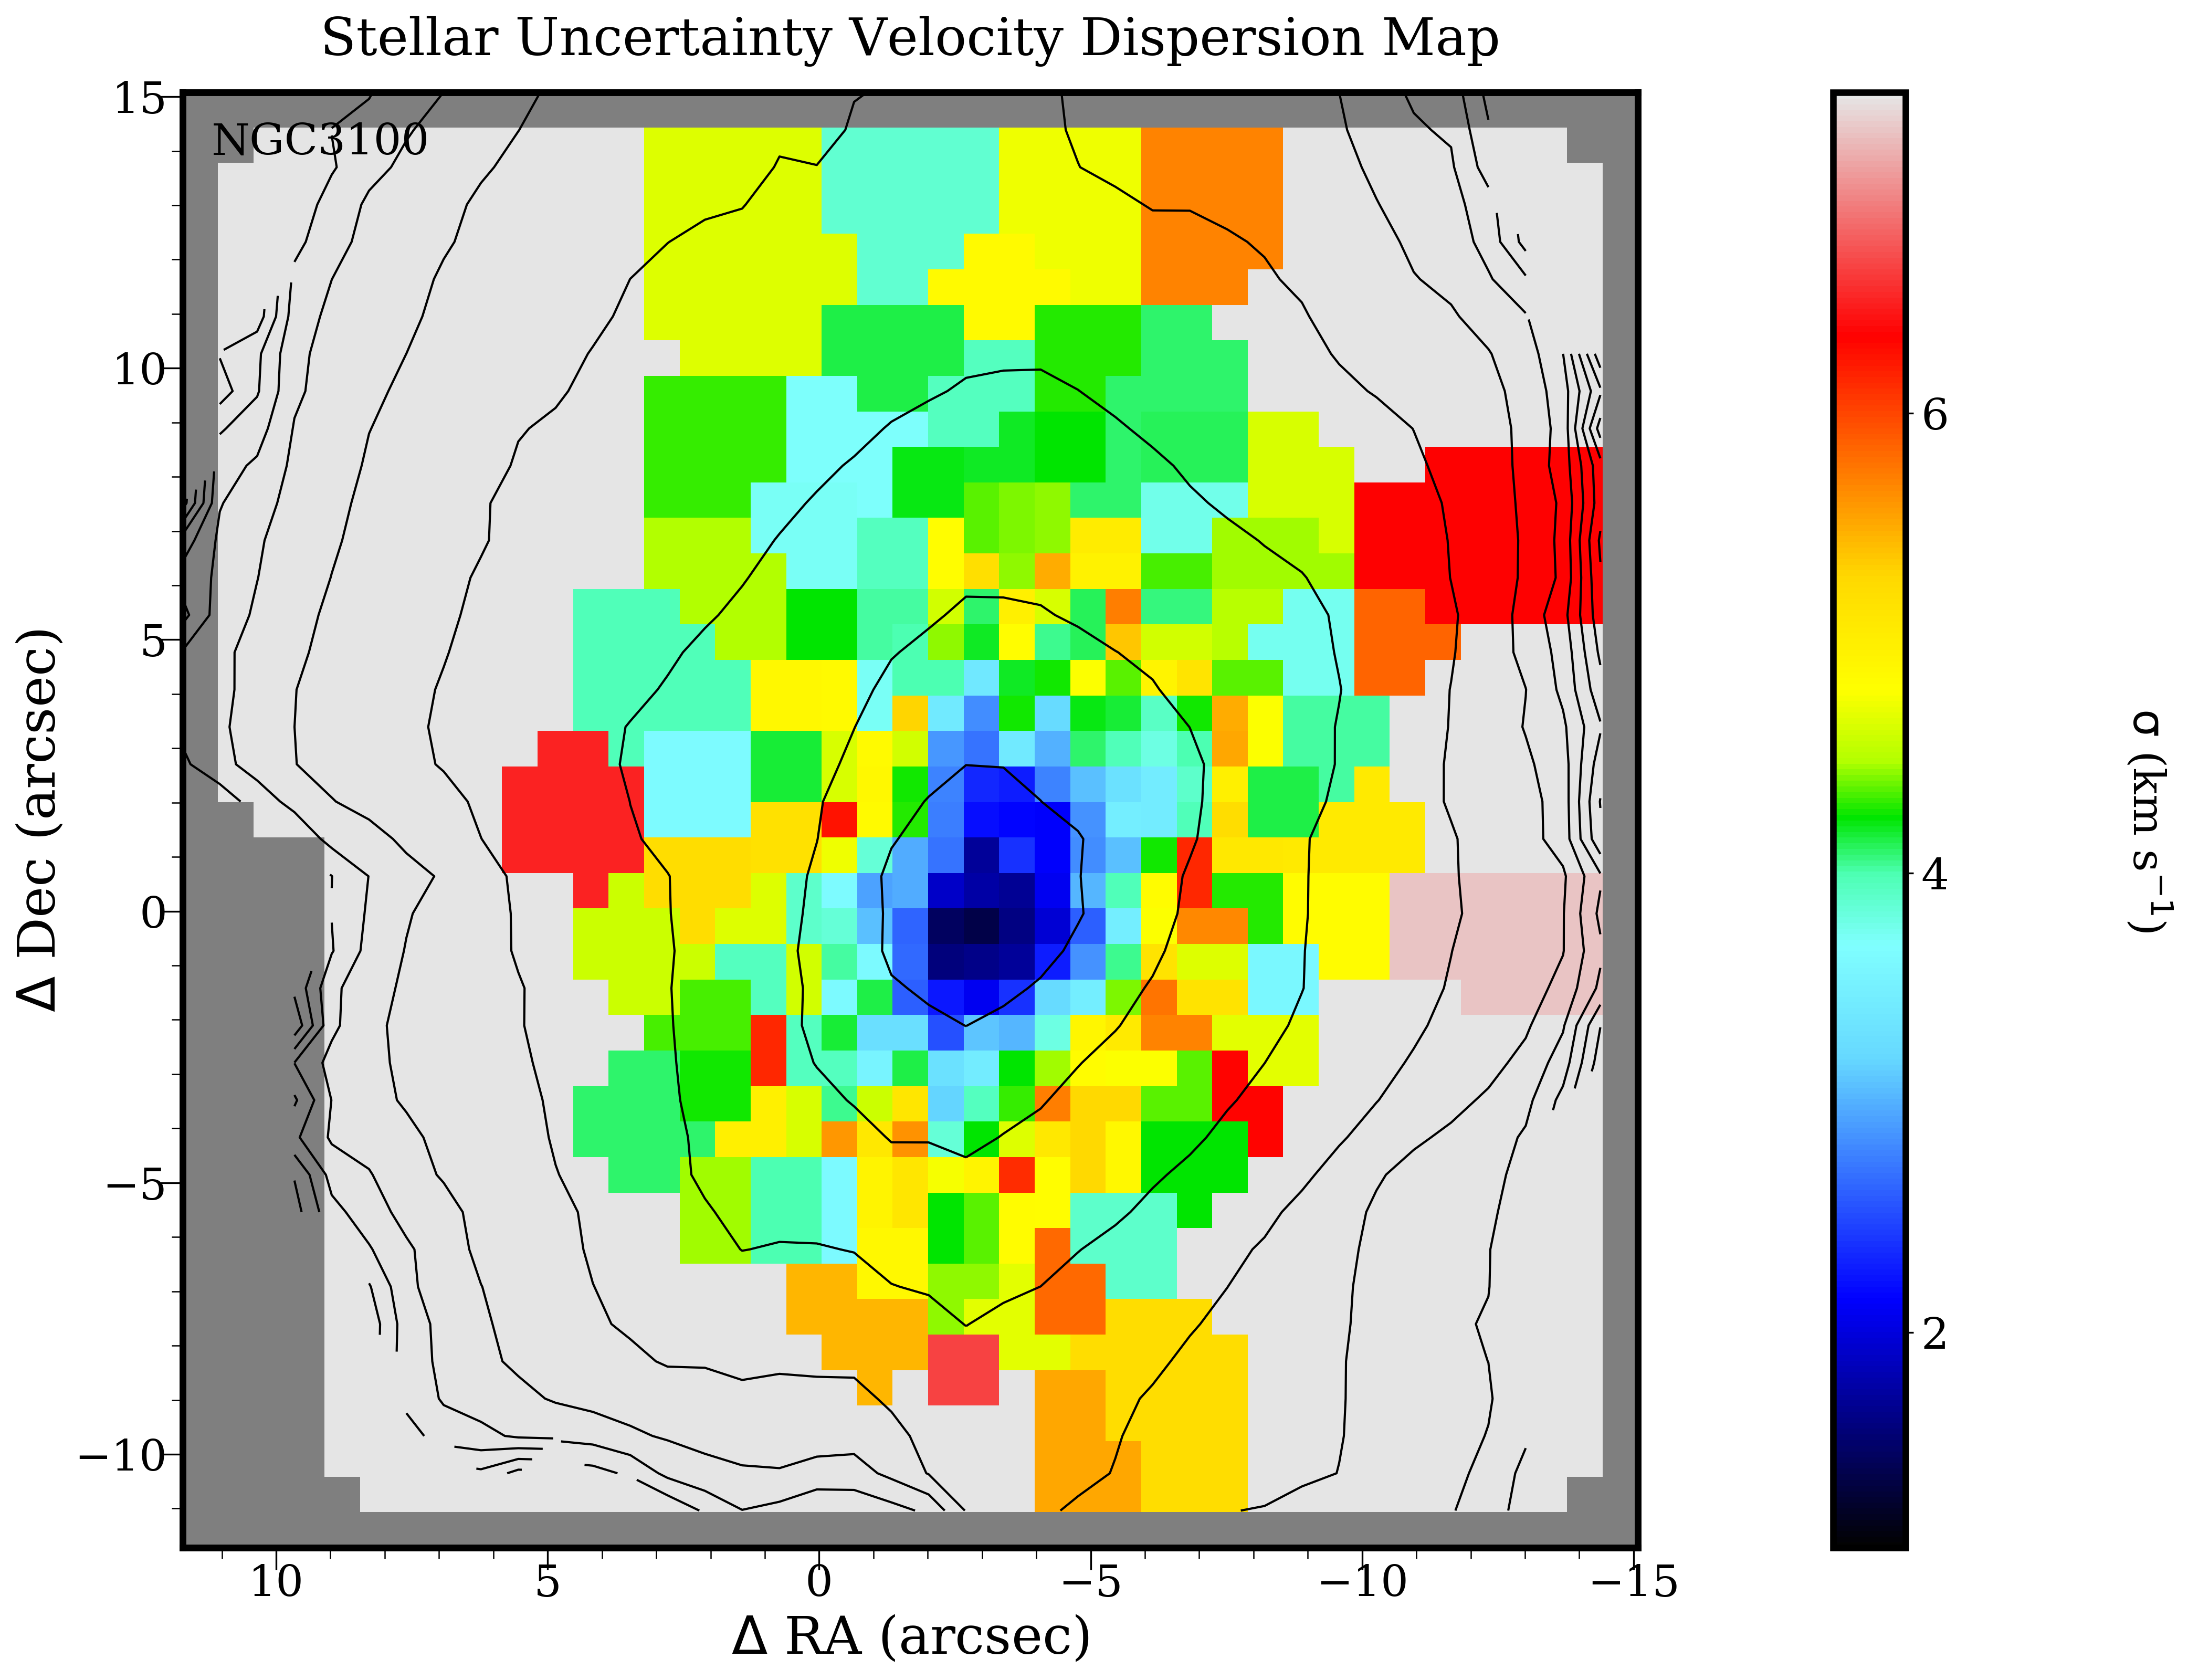
\includegraphics[width=0.245\textwidth]{Vmaps/ngc3100_stellar_sigma_uncert.png}
      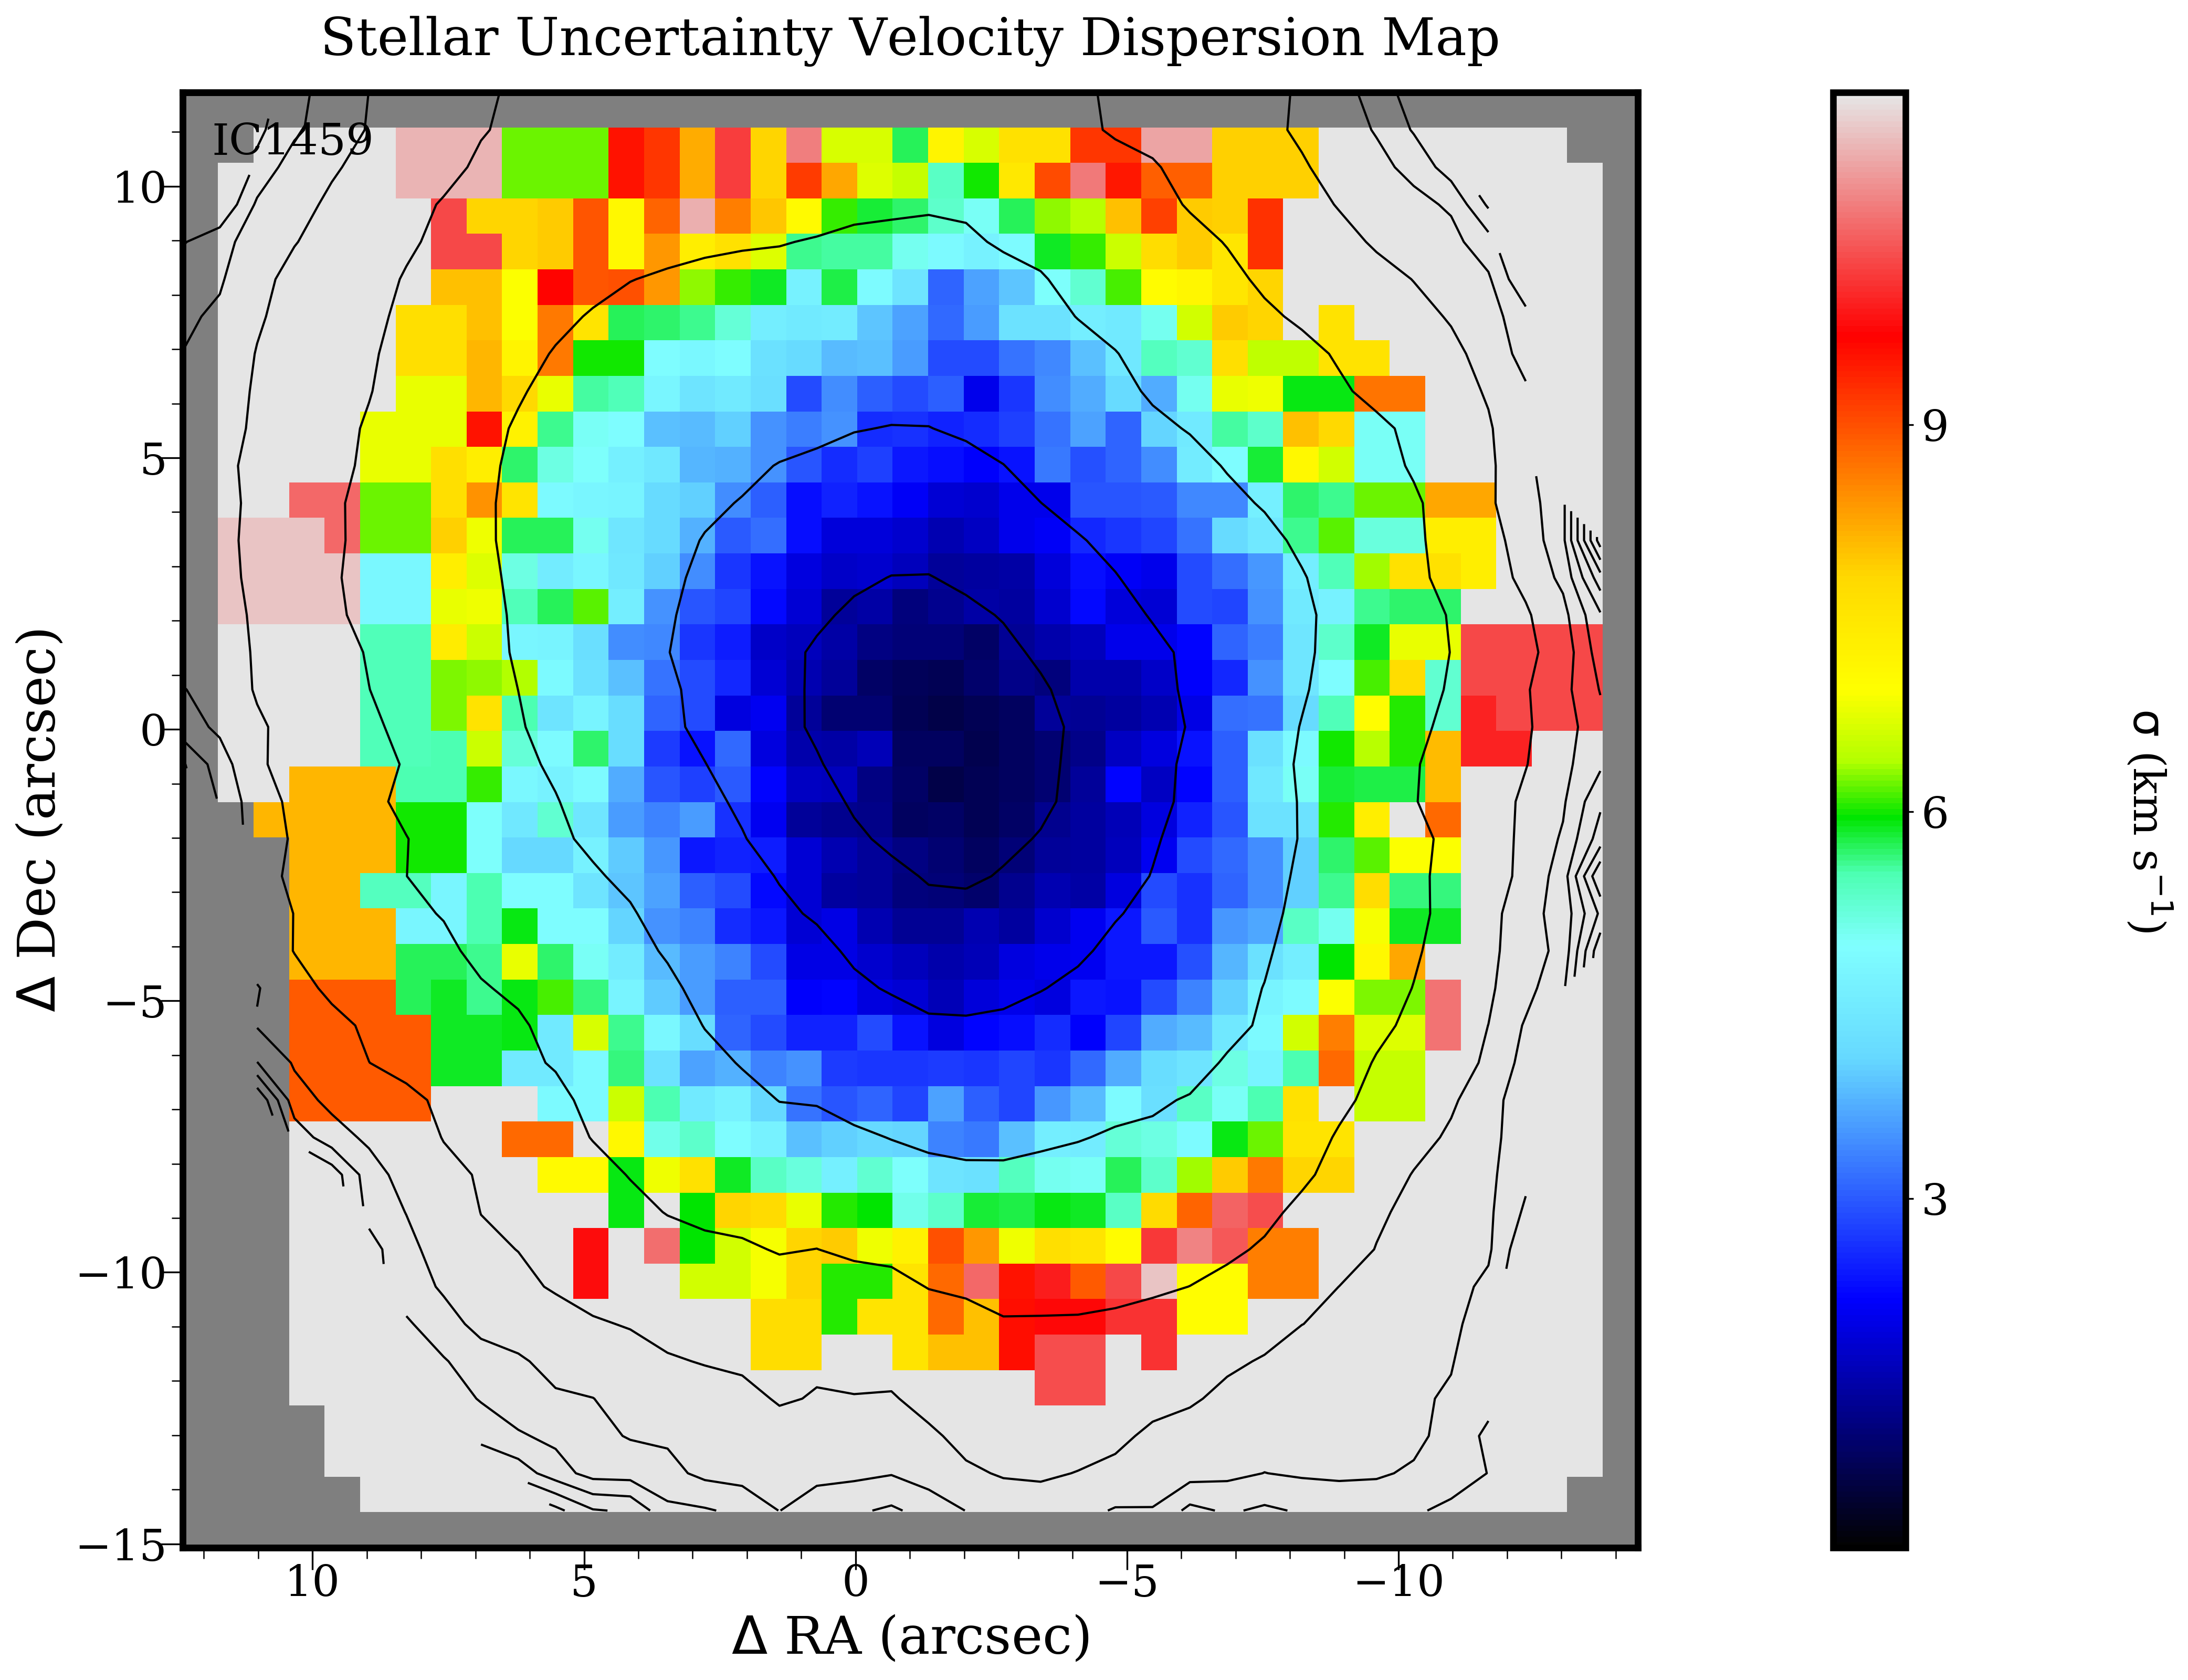
\includegraphics[width=0.245\textwidth]{Vmaps/ic1459_stellar_sigma_uncert.png}
      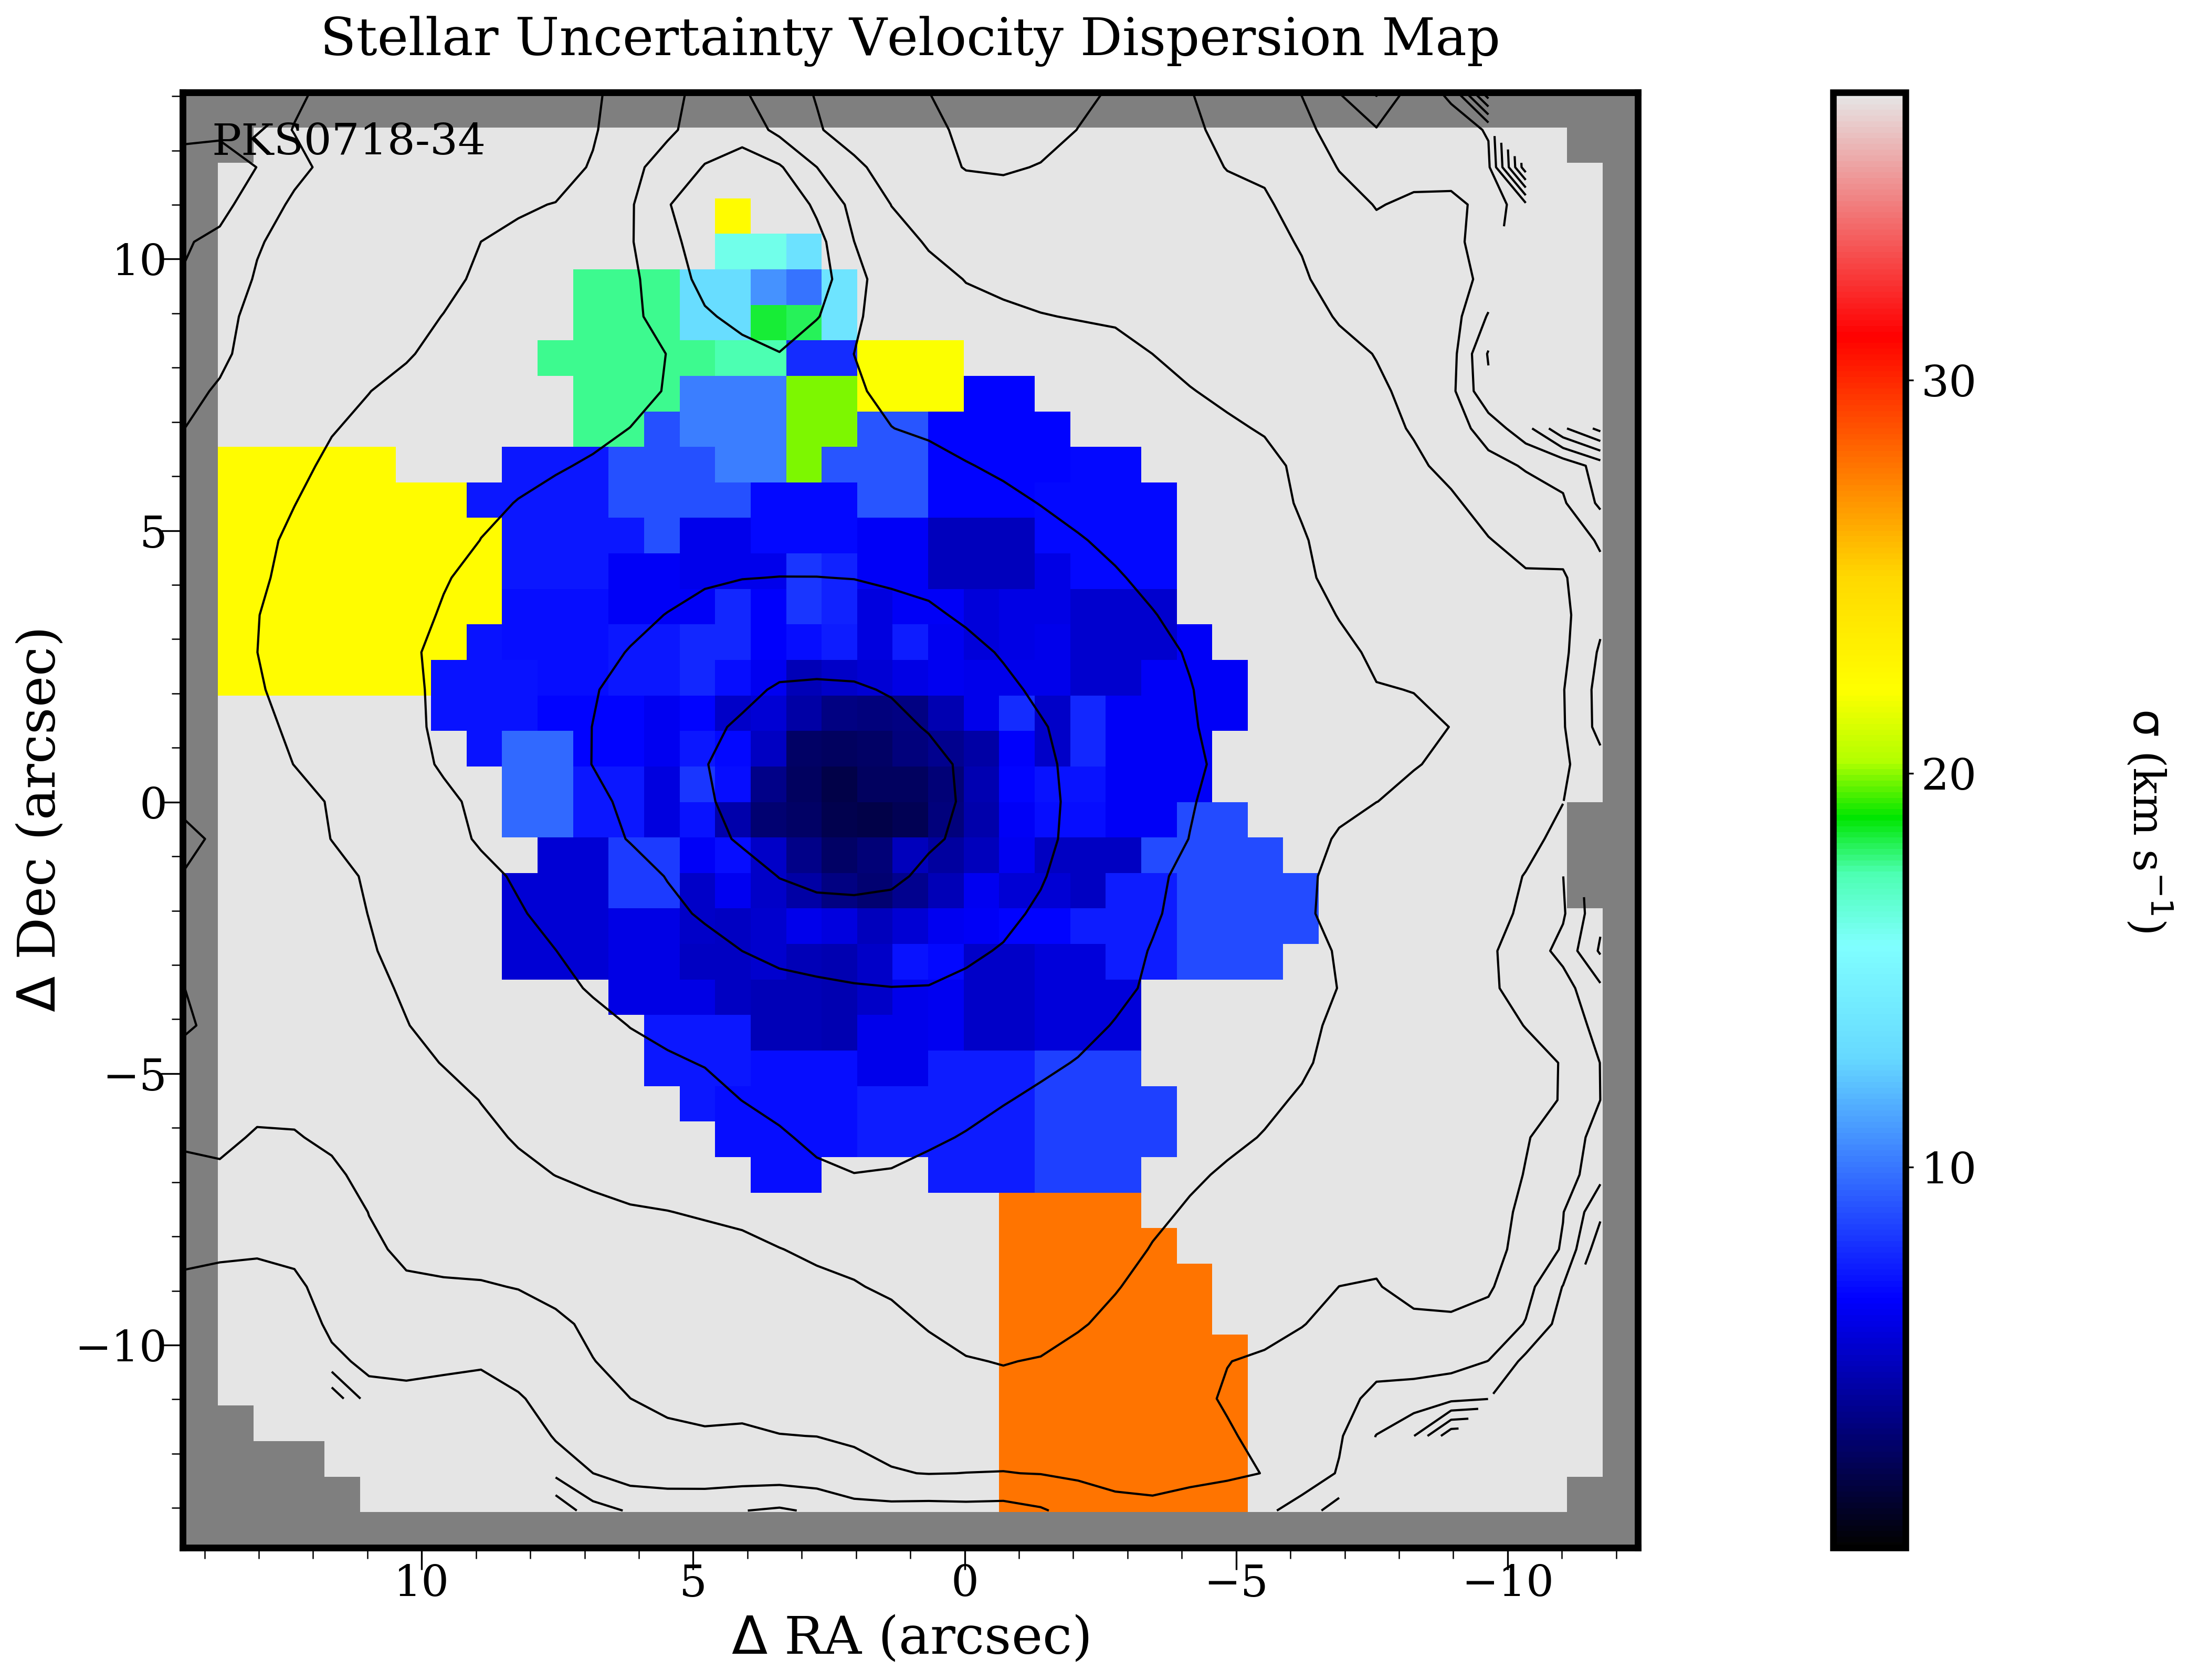
\includegraphics[width=0.245\textwidth]{Vmaps/pks0718-34_stellar_sigma_uncert.png}
      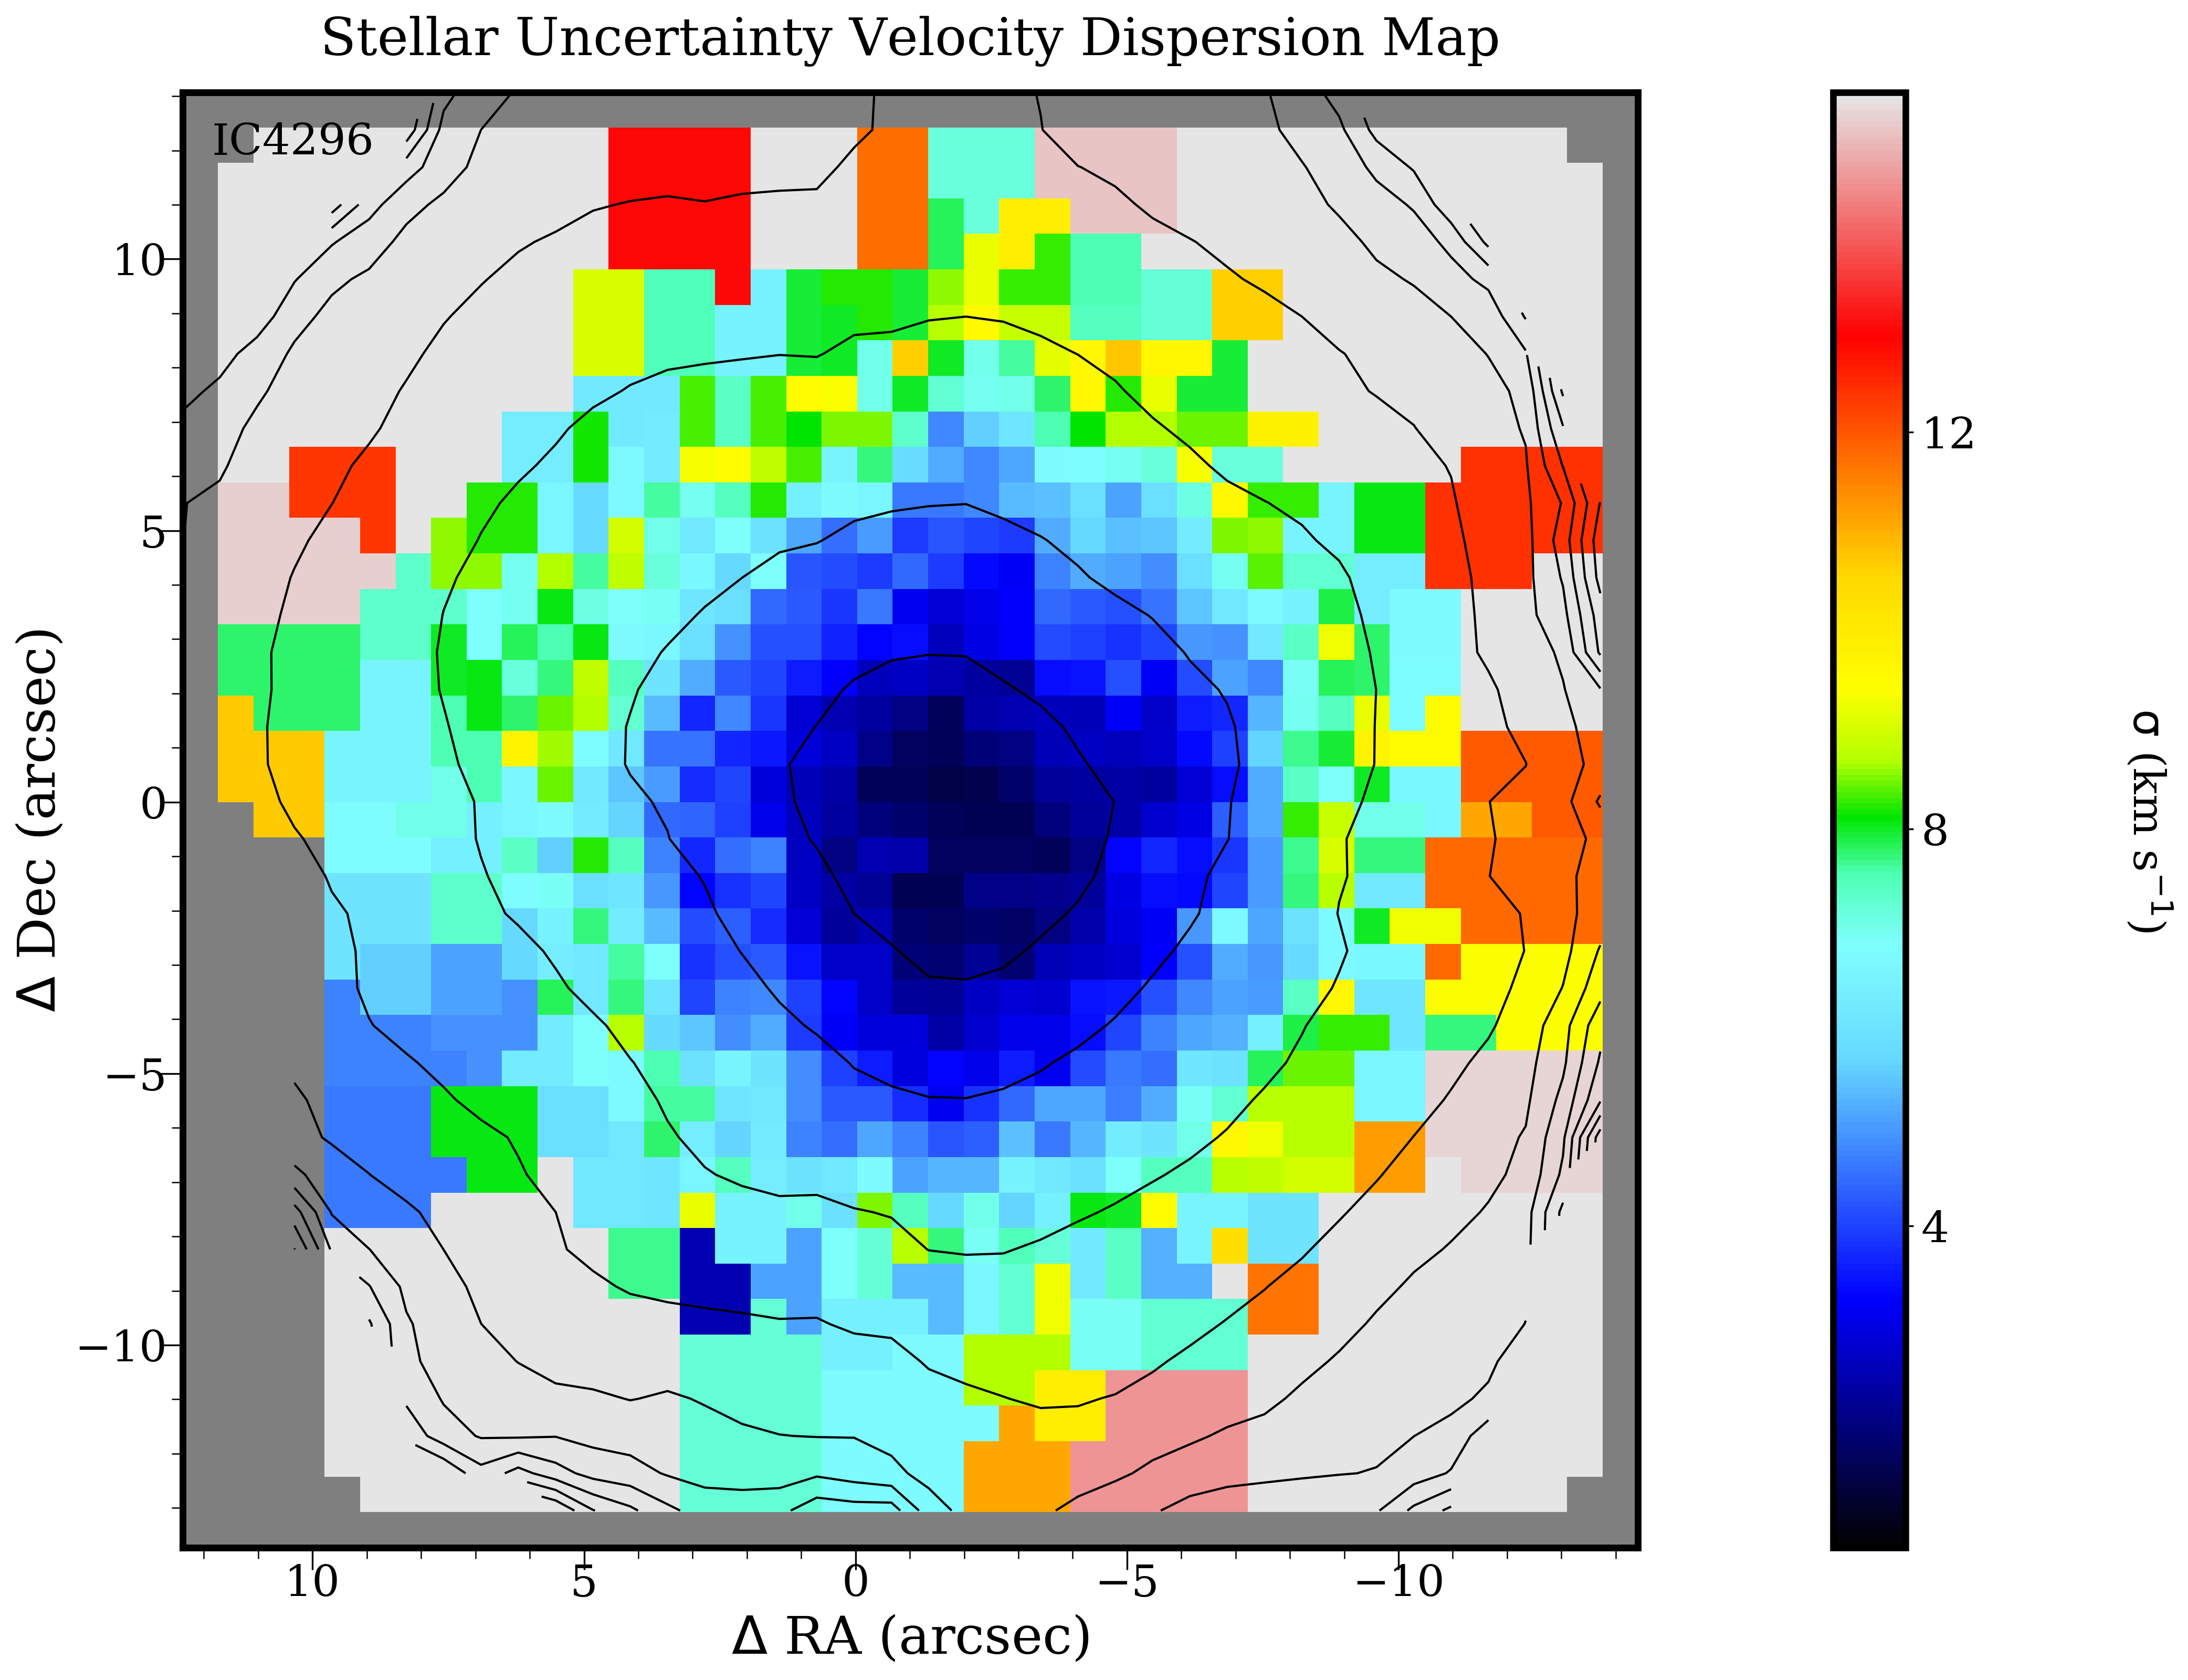
\includegraphics[width=0.245\textwidth]{Vmaps/ic4296_stellar_sigma_uncert.png}
      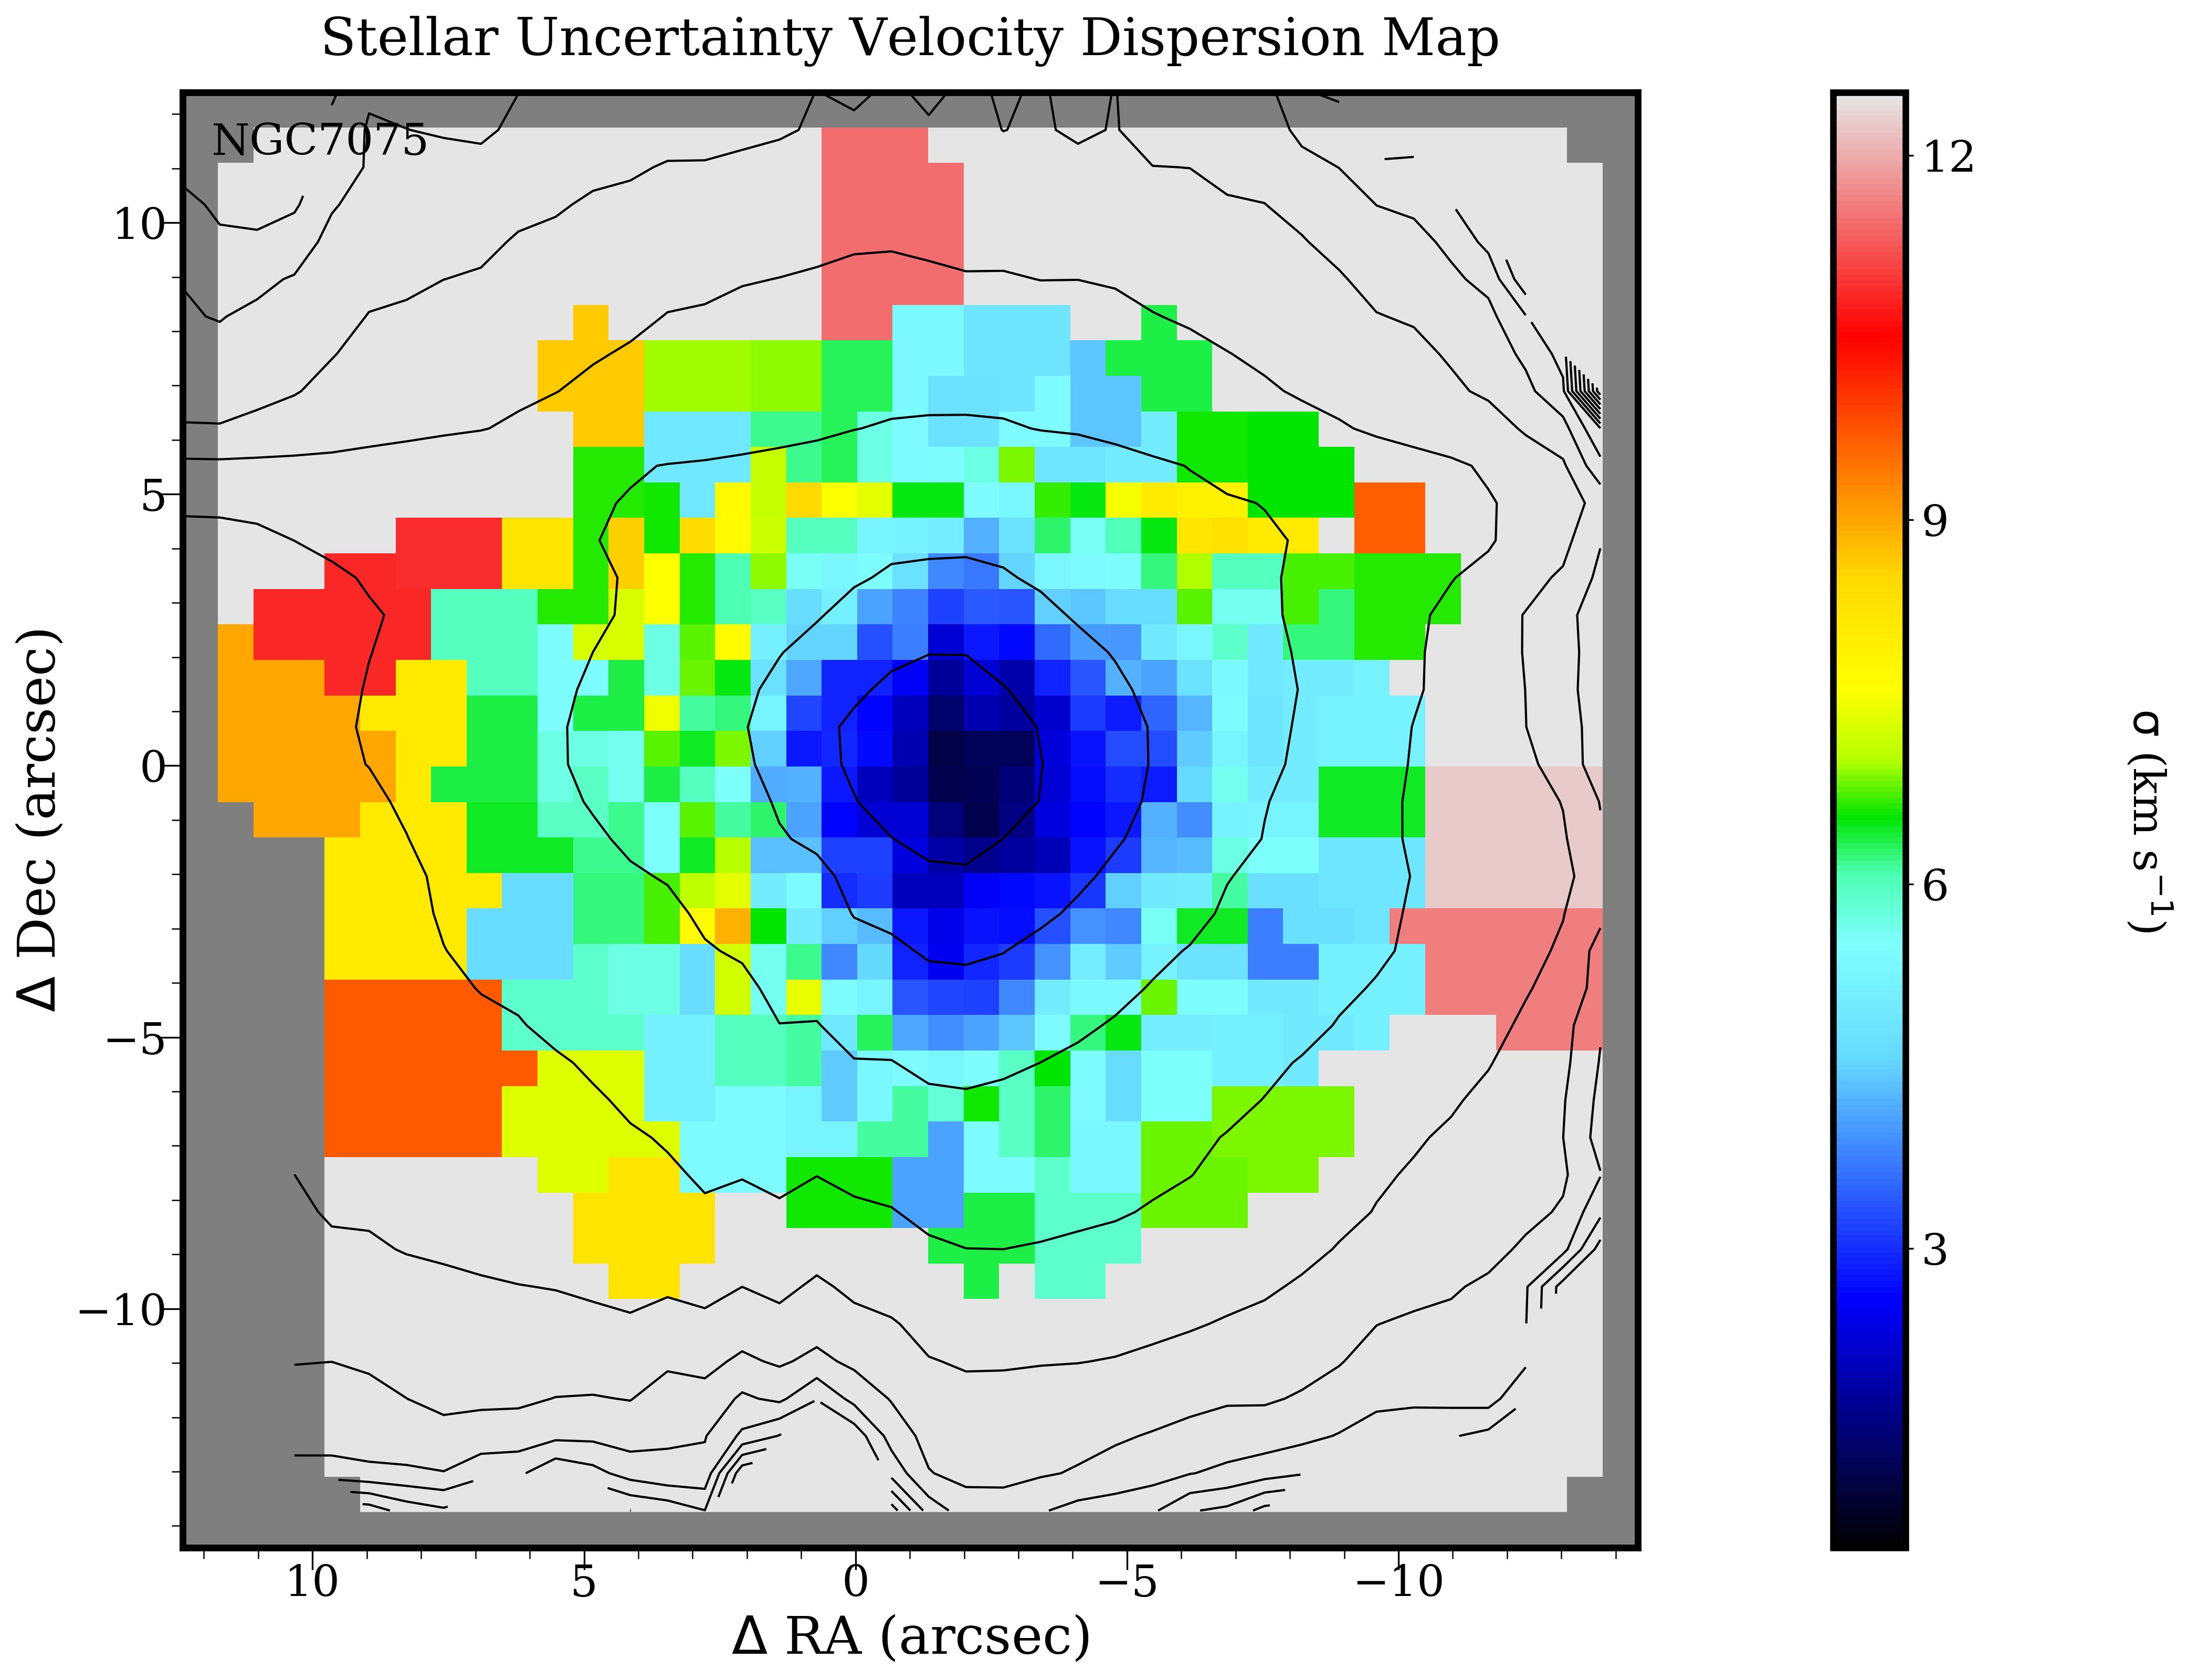
\includegraphics[width=0.245\textwidth]{Vmaps/ngc7075_stellar_sigma_uncert.png}
      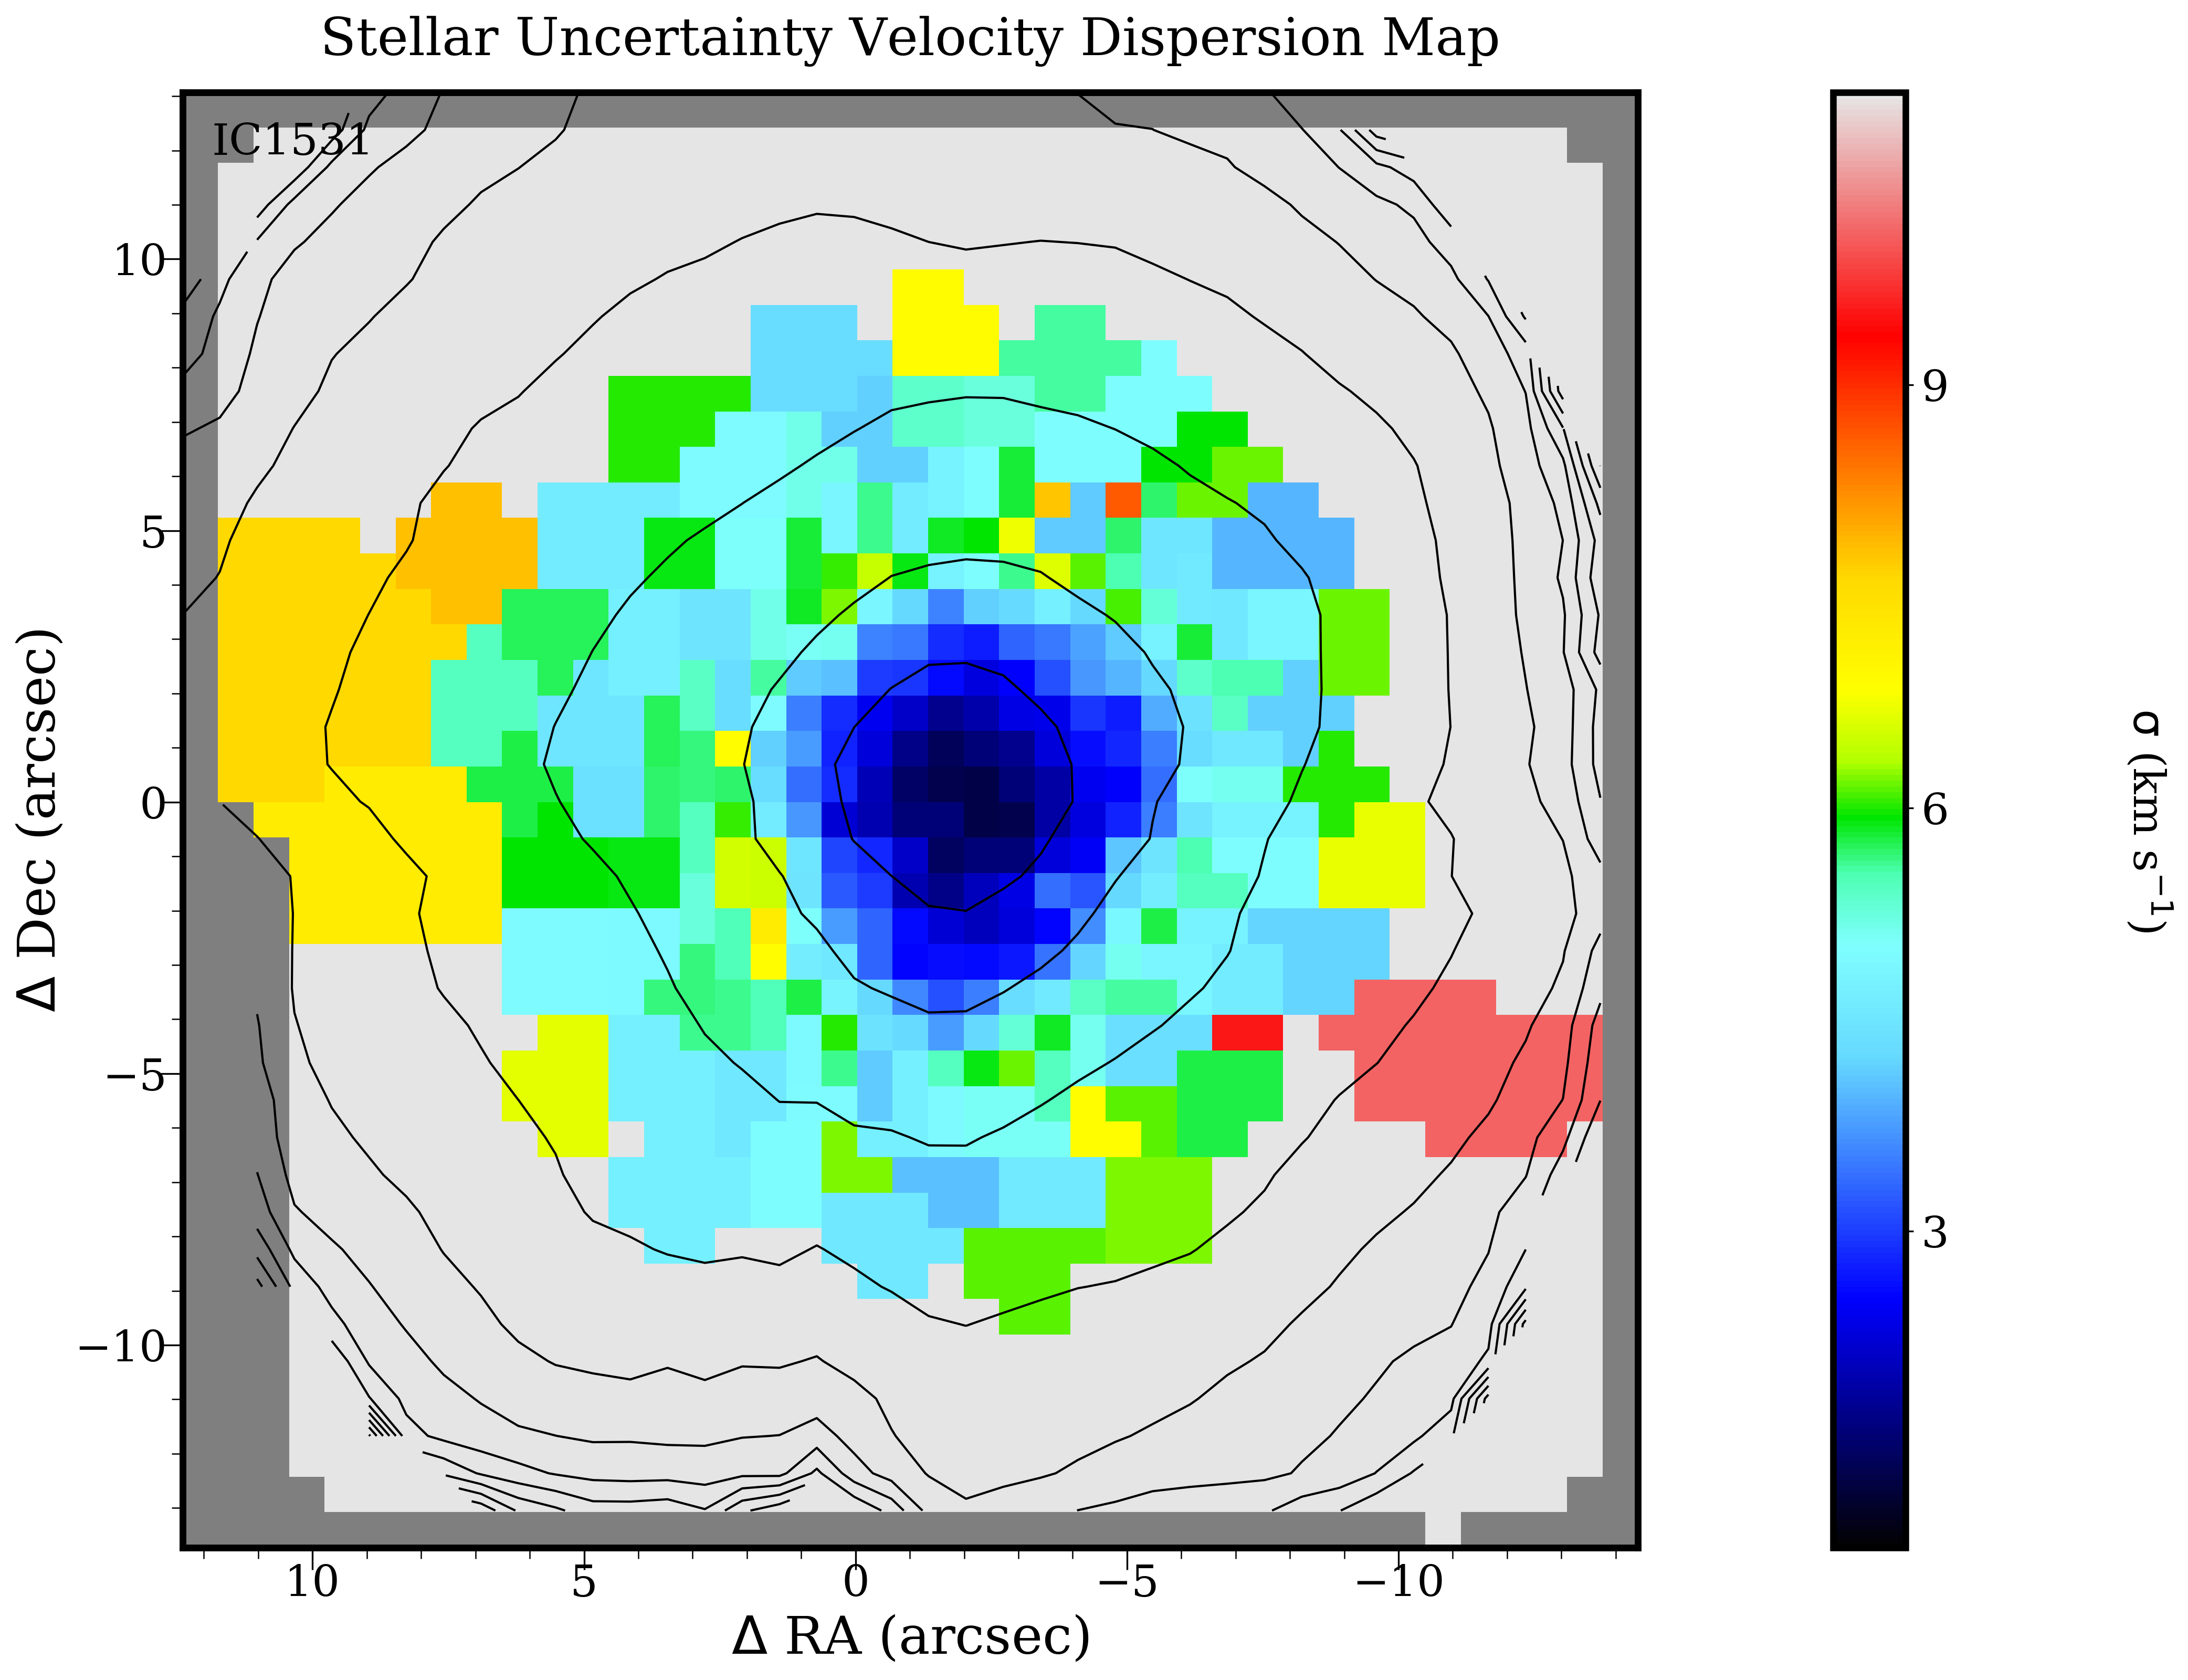
\includegraphics[width=0.245\textwidth]{Vmaps/ic1531_stellar_sigma_uncert.png}
      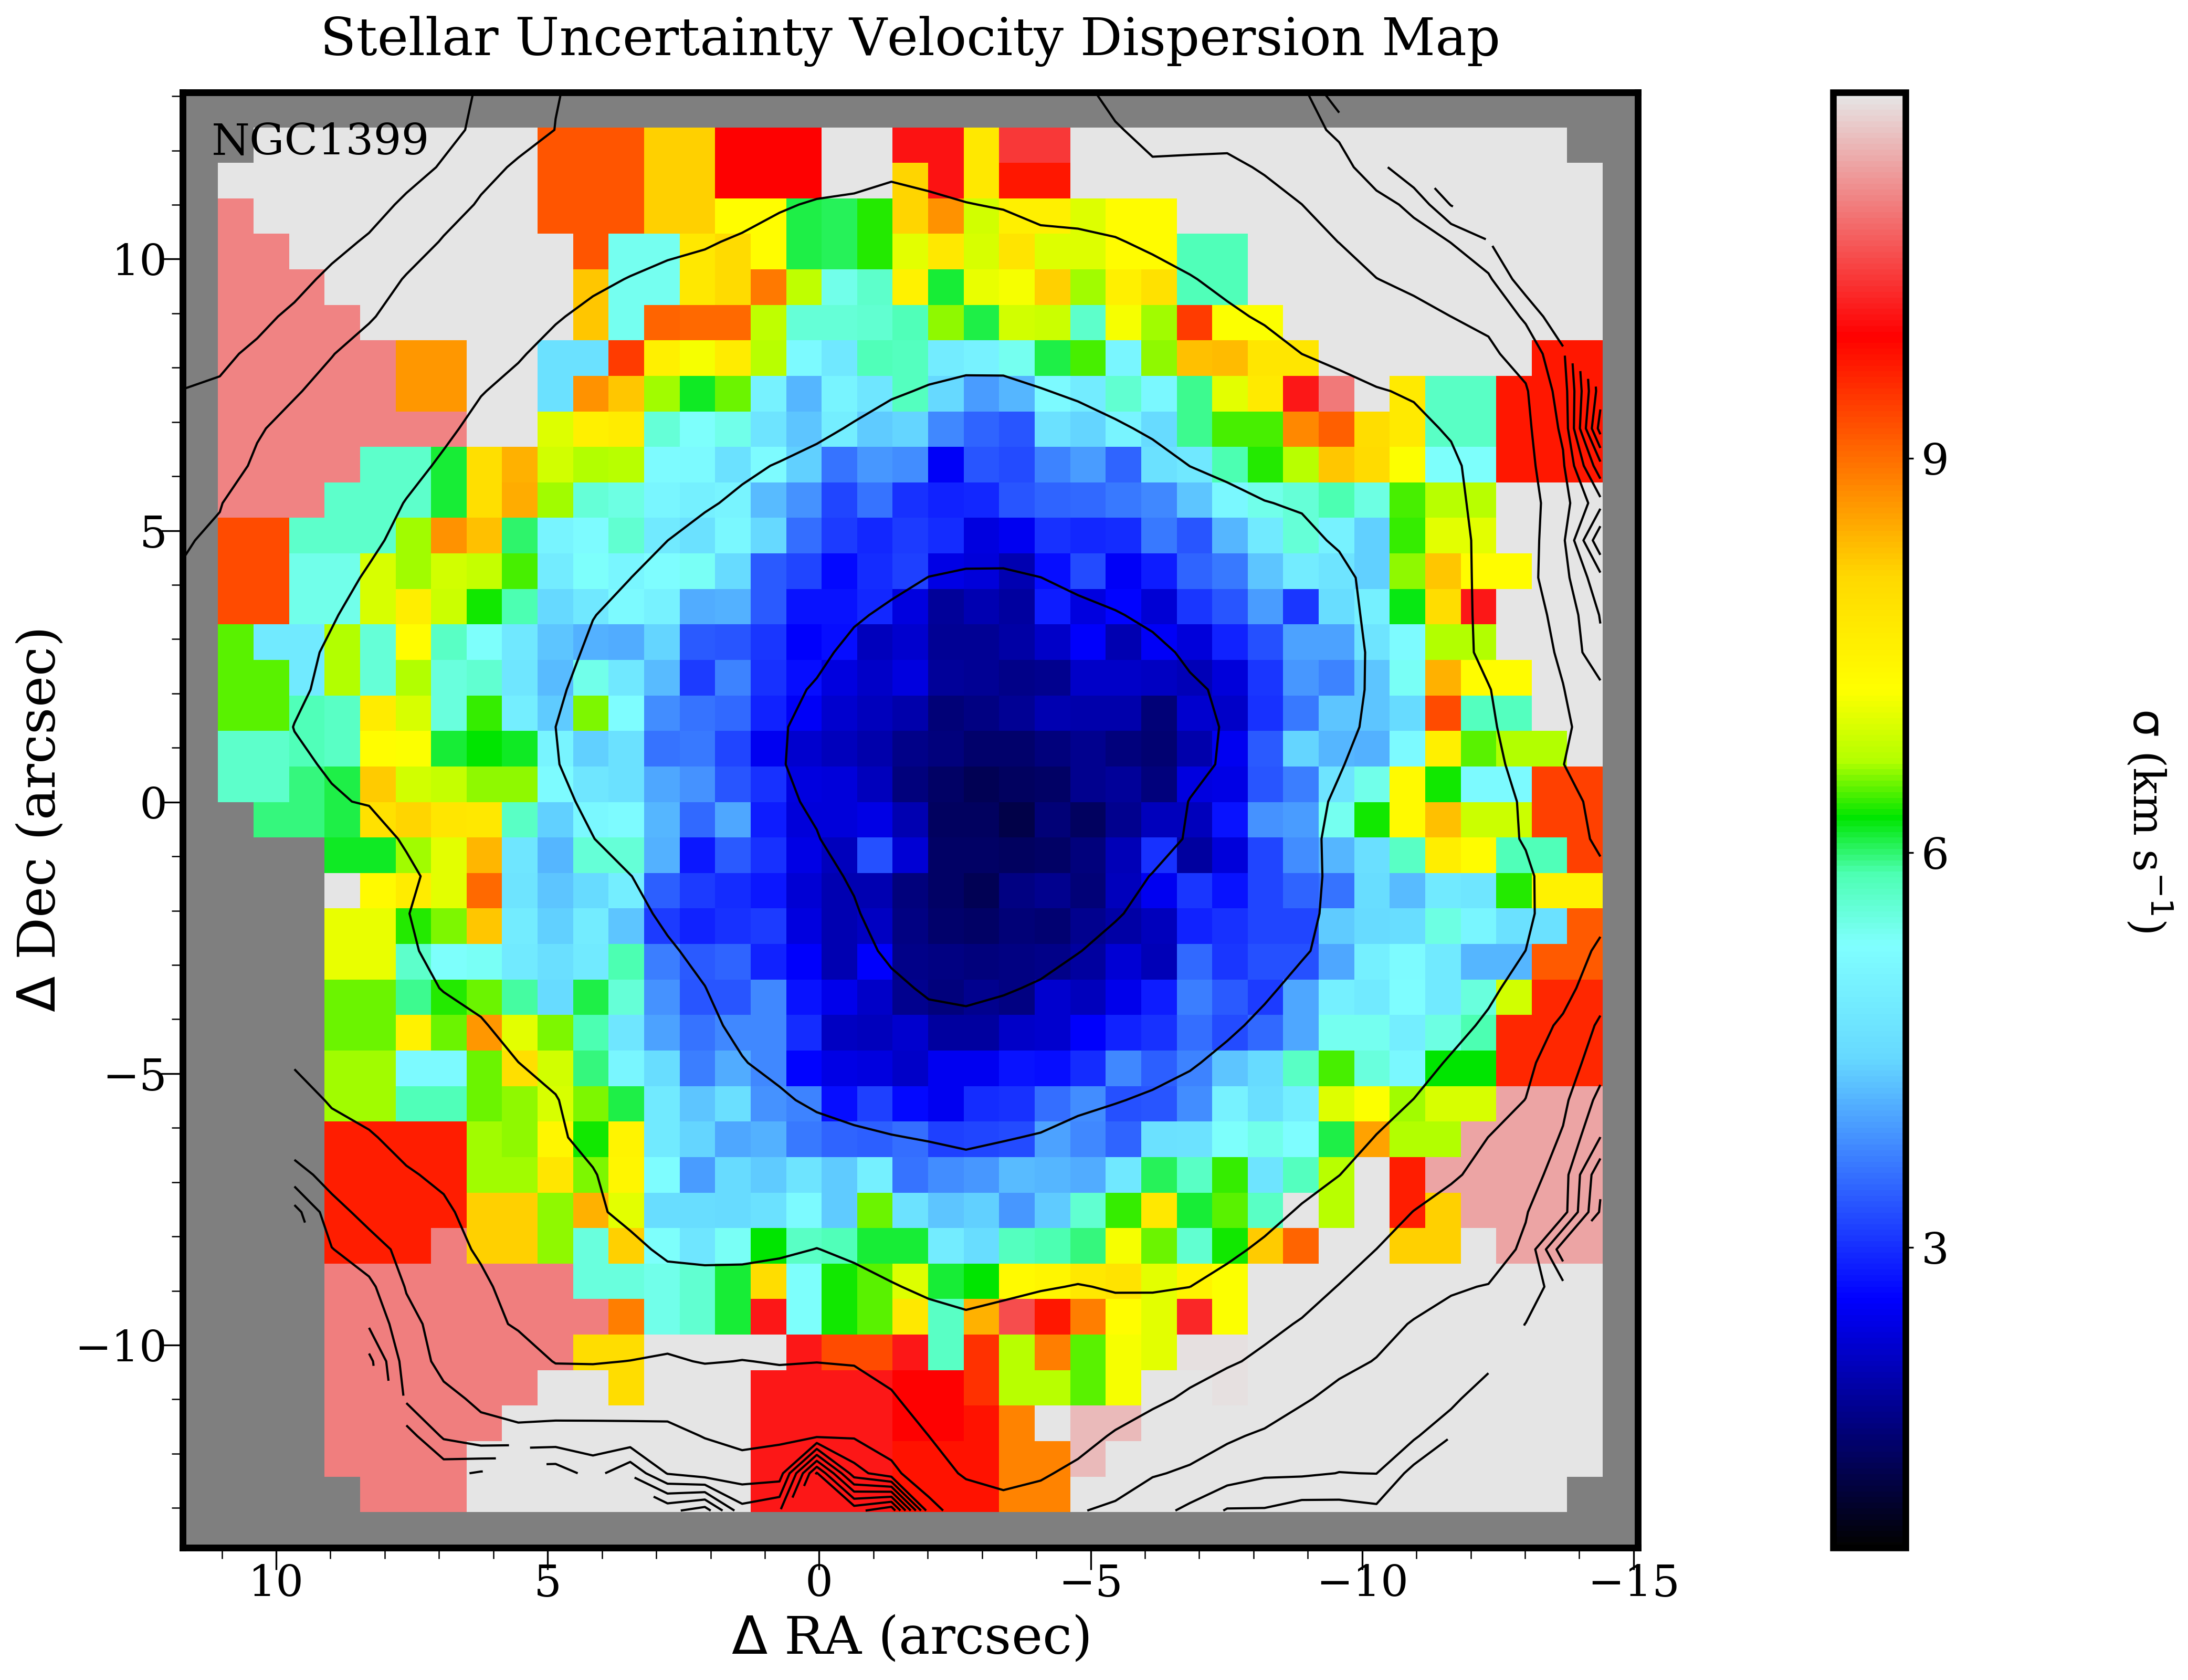
\includegraphics[width=0.245\textwidth]{Vmaps/ngc1399_stellar_sigma_uncert.png}
      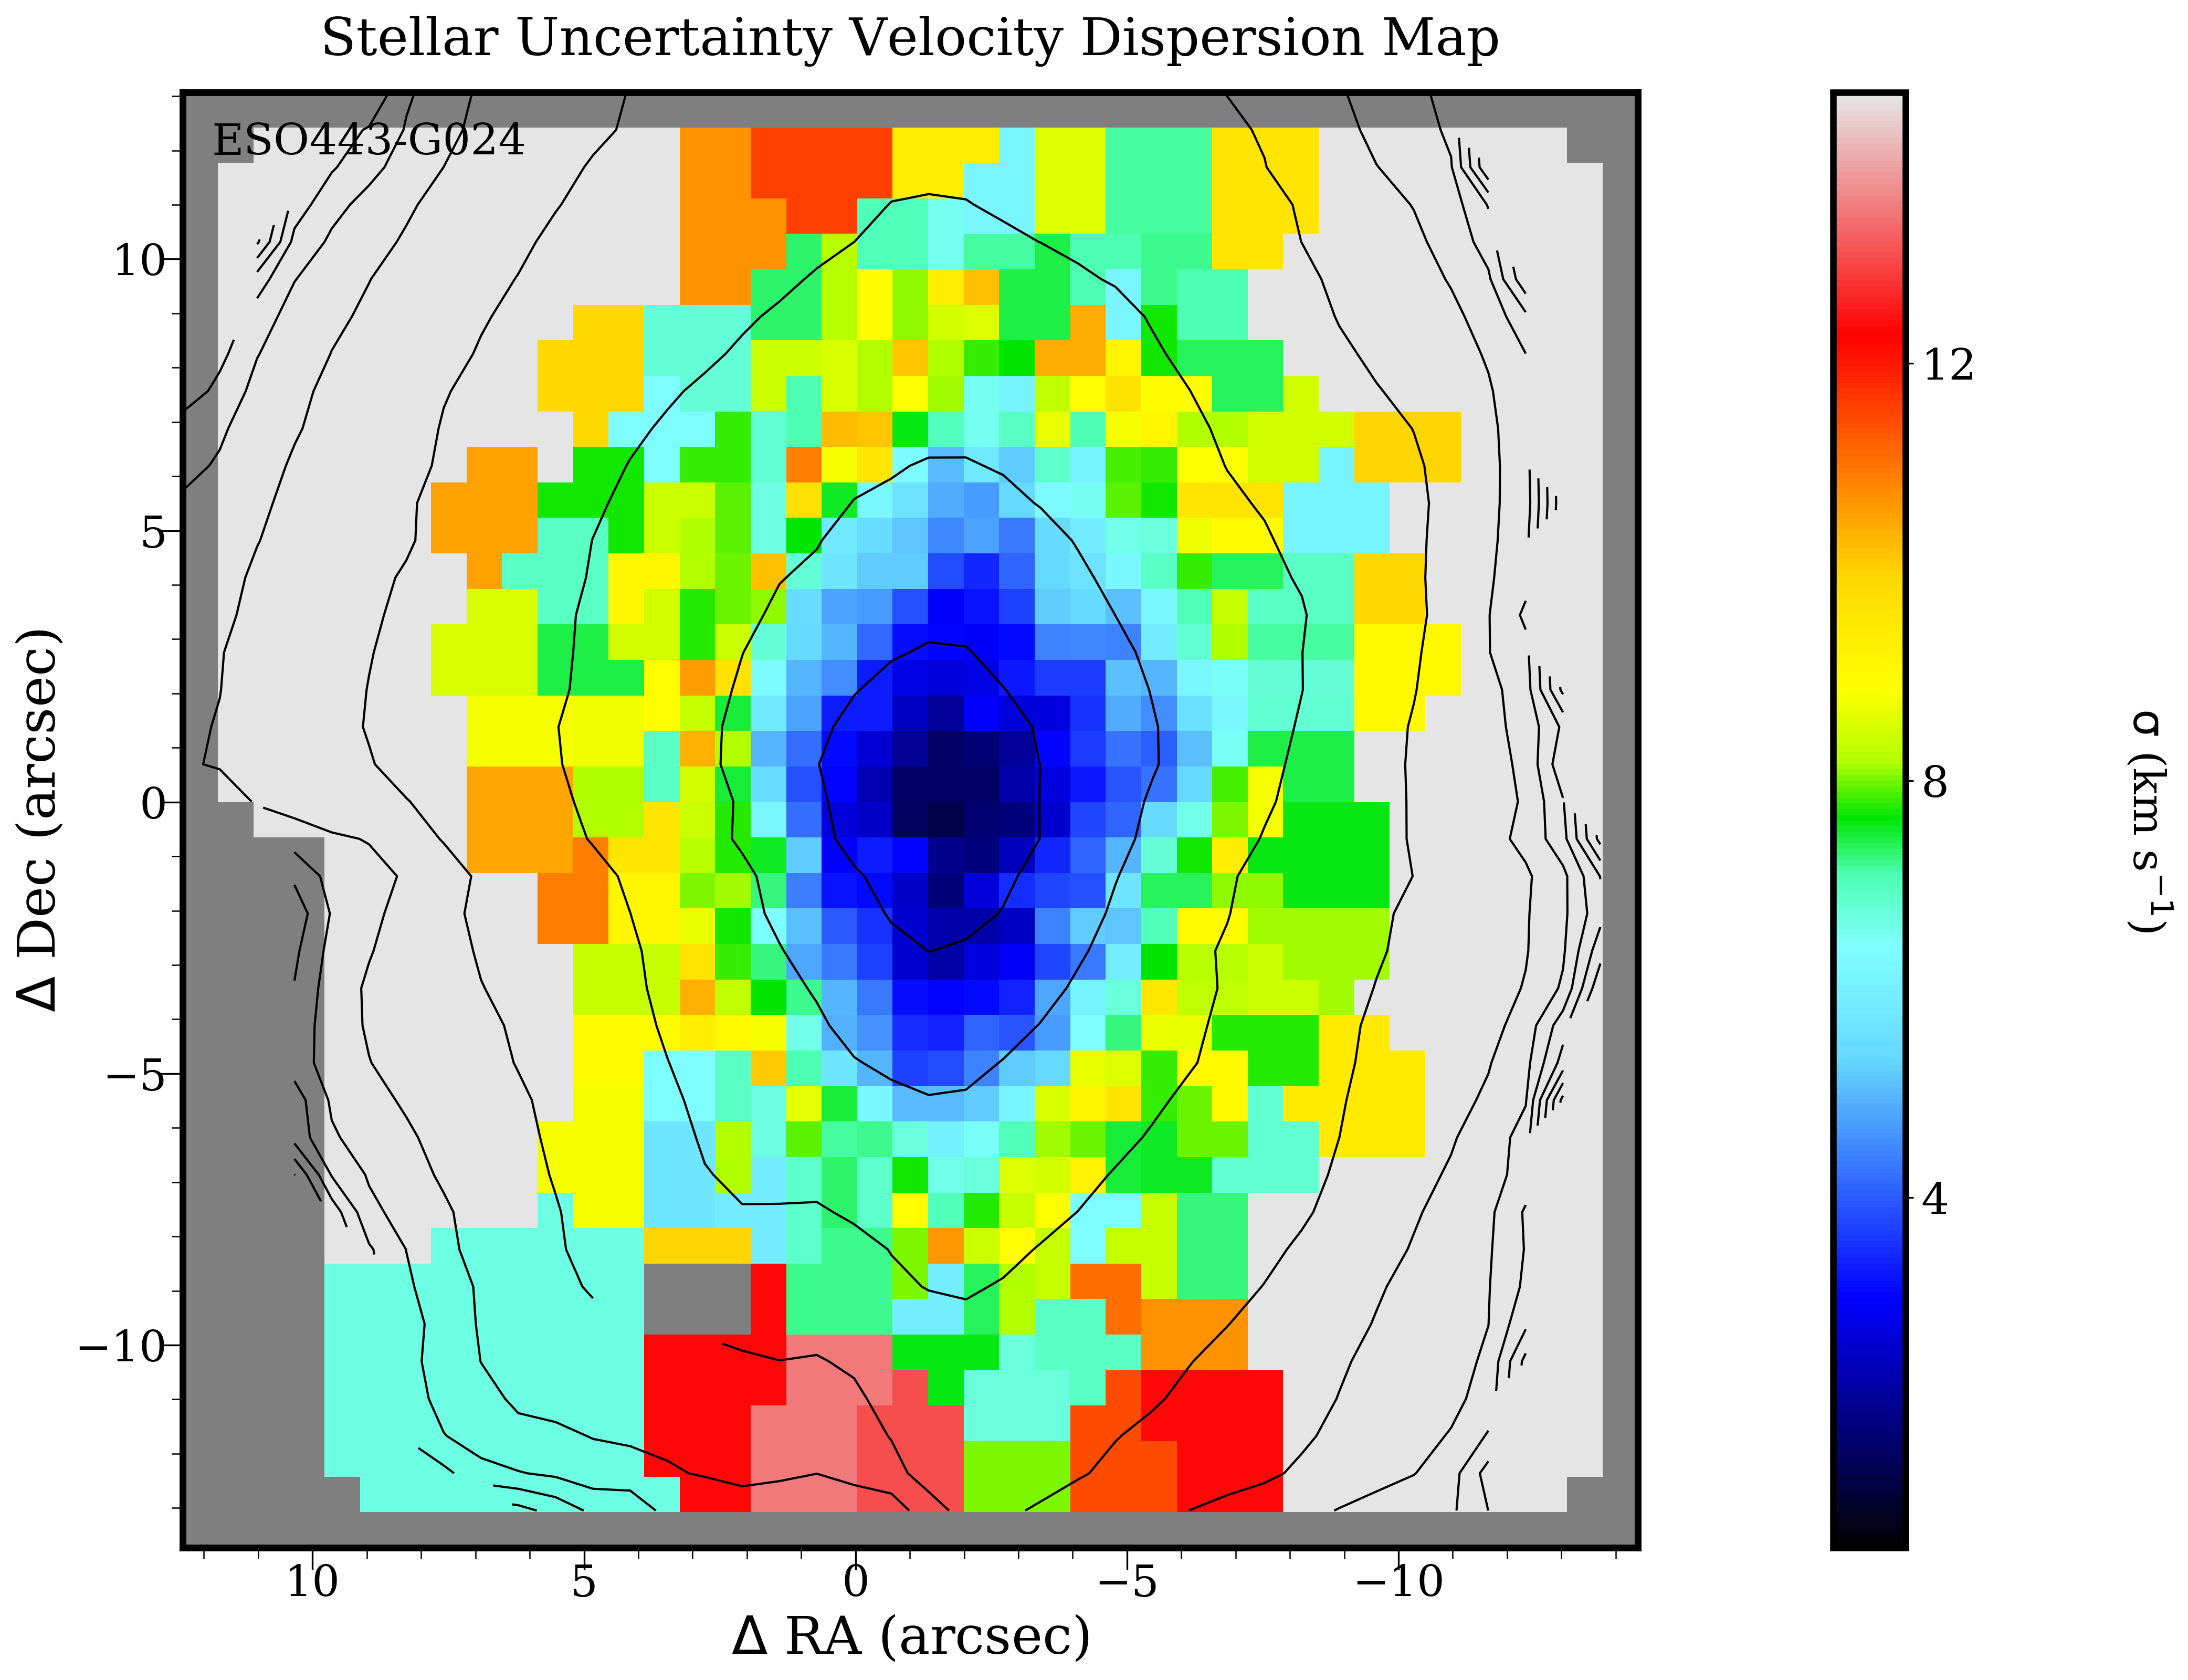
\includegraphics[width=0.245\textwidth]{Vmaps/eso443-g024_stellar_sigma_uncert.png}
      \caption[VIMOS dispersion uncertocity maps]{Uncertainties in the velocity dispersion for each galaxy in the VIMOS sample. Plots are ordered and contour colors are as in figure \ref{fig:Vstellar_img}}
      \label{fig:Vstellar_sigma_uncert}
\end{figure*}






\begin{figure*}
      \centering
      \includegraphics[width=0.245\textwidth]{Mmaps/ic1459_stellar_img.png}
      \includegraphics[width=0.245\textwidth]{Mmaps/ngc1316_stellar_img.png}
      \includegraphics[width=0.245\textwidth]{Mmaps/ic4296_stellar_img.png}
      \includegraphics[width=0.245\textwidth]{Mmaps/ngc1399_stellar_img.png}
      \caption[MUSE images]{Image for each galaxy in the MUSE sample. Plots are ordered roughly in peak stellar velocity with the contours as in figure \ref{fig:Vstellar_img}}
      \label{fig:Mstellar_img}
\end{figure*}

\begin{figure*}
      \centering
      \includegraphics[width=0.245\textwidth]{Mmaps/ic1459_stellar_vel.png}
      \includegraphics[width=0.245\textwidth]{Mmaps/ngc1316_stellar_vel.png}
      \includegraphics[width=0.245\textwidth]{Mmaps/ic4296_stellar_vel.png}
      \includegraphics[width=0.245\textwidth]{Mmaps/ngc1399_stellar_vel.png}
      \caption[MUSE velocity maps]{Velocity for each galaxy in the MUSE sample. Plots are ordered as in figure \ref{fig:Mstellar_img} and contour colors are as in figure \ref{fig:Vstellar_img}}
      \label{fig:stellar_vel}
\end{figure*}

\begin{figure*}
      \centering
      \includegraphics[width=0.245\textwidth]{Mmaps/ic1459_stellar_vel_uncert.png}
      \includegraphics[width=0.245\textwidth]{Mmaps/ngc1316_stellar_vel_uncert.png}
      \includegraphics[width=0.245\textwidth]{Mmaps/ic4296_stellar_vel_uncert.png}
      \includegraphics[width=0.245\textwidth]{Mmaps/ngc1399_stellar_vel_uncert.png}
      \caption[MUSE velocity uncertocity maps]{Uncertainties in the velocity for each galaxy in the MUSE sample. Plots are ordered as in figure \ref{fig:Mstellar_img} and contour colors are as in figure \ref{fig:Vstellar_img}}
      \label{fig:Mstellar_vel_uncert}
\end{figure*}

\begin{figure*}
      \centering
      \includegraphics[width=0.245\textwidth]{Mmaps/ic1459_stellar_sigma.png}
      \includegraphics[width=0.245\textwidth]{Mmaps/ngc1316_stellar_sigma.png}
      \includegraphics[width=0.245\textwidth]{Mmaps/ic4296_stellar_sigma.png}
      \includegraphics[width=0.245\textwidth]{Mmaps/ngc1399_stellar_sigma.png}
      \caption[MUSE velocity dispersion]{Velocity dispersion for each galaxy in the MUSE sample. Plots are ordered as in figure \ref{fig:Mstellar_img} and contour colors are as in figure \ref{fig:Vstellar_img}}
      \label{fig:Mstellar_sigma}
\end{figure*}


\begin{figure*}
      \centering
      \includegraphics[width=0.245\textwidth]{Mmaps/ic1459_stellar_sigma_uncert.png}
      \includegraphics[width=0.245\textwidth]{Mmaps/ngc1316_stellar_sigma_uncert.png}
      \includegraphics[width=0.245\textwidth]{Mmaps/ic4296_stellar_sigma_uncert.png}
      \includegraphics[width=0.245\textwidth]{Mmaps/ngc1399_stellar_sigma_uncert.png}
      \caption[MUSE dispersion uncertocity maps]{Uncertainties in the velocity dispersion for each galaxy in the MUSE sample. Plots are ordered as in figure \ref{fig:Mstellar_img} and contour colors are as in figure \ref{fig:Vstellar_img}}
      \label{fig:Mstellar_sigma_uncert}
\end{figure*}

		Figures \ref{fig:Vstellar_img} - \ref{fig:Mstellar_sigma_uncert} show the stellar LOSVD with associated uncertainties for all VIMOS and MUSE datacubes. 

		The kinematics of the sample are classified according to the Regular-Rotator/Non Regular-Rotator (RR/NRR) regime given in \citet{Krajnovic2011}, Fast/Slow Rotator (FR/SR) regime given in \citet{Cappellari2016} (originally defined by \citet{Emsellem2011}, but later refined by \citet{Cappellari2016}). Beyond this attempts have been made to use the kinematic features as defined in \citet{Krajnovic2011}, however the quality of the data has meant that many have had to be classified by eye as the artifacts from the VIMOS quadrants confuse any ellipse fitting methods. In the following section (\ref{subsec:descriptions}) we will give a brief description of each galaxy with these classifications in mind. 

	\subsection{Galaxy descriptions}
		\label{subsec:descriptions}

		\textbf{ESO 443-G024} is consistent with a NR. It has a very dispersed H$_\mathrm{\beta}$ (similar to NGC 3557 (Fig. \ref{fig:Hbeta_eqW})).

		\textbf{IC 1459} is known to contain a KDC. This is clearly seen in both the VIMOS and MUSE velocity maps (Fig. \ref{fig:stellar_vel}, \ref{fig:MUSEstellar_vel}). It is also known to have ionized gas counter rotating to the decoupled core. This is again seen by comparing Fig. \ref{fig:stellar_vel} with \ref{fig:gas_vel} and \ref{fig:MUSEstellar_vel} with \ref{fig:MUSEgas_vel}. From the MUSE velocity maps it can be seen that the gas is not coupled to the outer parts of the galaxy either. The KDC appears to be embedded in a slow rotator, though the KDC contaminates the $\lambda_{Re}$ measurement such that it is classified as a Fast Rotator. This is consistent with Section \ref{subsec:KDCsize}.

		\textbf{IC 1531} seems to contain a KT. This galaxy has a very limited detection of ionized gas concentrated in the center (with the exception of [NI] (Fig. \ref{fig:NI_eqW}), which is more dispersed).

		\textbf{IC 4296} appears to have KT, though this may be a quadrant feature. There is potentially 2 peaks in all of the gas intensity maps, one at the center of the galaxy and one to the south-east which is not seen in the image (total flux/collapsed cube).

		\textbf{NGC 0612} has a large dust lane to the east of the apparent center of the galaxy perpendicular to the axis of rotation. The dust lane is also seen as a lower velocity dispersion (Fig \ref{fig:stellar_sigma}). Dust lanes generally imply a disky galaxy: indeed this seems to be the case here as the dust lane is aligned with the plane of the disk. The kinematic maps show NF. The dust lane also contains large amounts of gas. 

		\textbf{NGC1316} (Fornax A) was not observed with VIMOS, however the MUSE maps show it to have a clear rotation signature (Fig. \ref{fig:MUSEstellar_vel}), though disturbed kinematics (e.g. Fig. \ref{fig:MUSEstellar_sigma}). The ionized gas is very clumpy and has no rotation (Fig. \ref{fig:MUSEgas_vel}).

		\textbf{NGC 1399}, the central galaxy of the Fornax Cluster \citep{Jordan2007}, is known to have kinematic twist (see MUSE map in \citet{Zieleniewski2017}) on the scale of our MUSE field of view (reduced to 30"). Very little ionized gas was detected. 

		\textbf{NGC 3100} is has NF in the stellar kinematics, however there is significant amount of ionized gas, which seems to be split into two clouds. This is most obviously seen in Fig. \ref{fig:Hbeta_eqW}. The gas also seems to have a non-standard rotation, possibly linked to its spacial distribution. 

		\textbf{NGC 3557} is known to be FR with very high velocities, especially considering it's size, with NF. In our maps, there some significant quadrant effects. NGC 3557 also has a very dispersed, non-centrally concentrated H$_\mathrm{\beta}$ distribution. 

		\textbf{NGC 7075} appears to have NF, though with quite slow velocities. There is some H$_\mathrm{\beta}$ detected at the very center of the galaxy. 

		\textbf{PKS 0718-34} is a KDC, though S/N issues mean that as in IC 1459, the galaxy cannot be seen beyond the core. It has very little gas detected, though the often faint $H_\mathrm{\delta}$ line is detected. [NI] is redshifted out of the VIMOS spectral range.

		








\section{Stellar Population}
	\label{sec:pop}




	\subsection{Kinematically Decoupled Cores}
		\label{sec:popKDC}

	\section{The case of NGC 612}
		\label{sec:NGC612}